\documentclass[12pt]{article}
\usepackage{a4wide}
\usepackage{amsmath,amssymb}
\usepackage{bm}
\usepackage[colorlinks]{hyperref}
\usepackage{graphicx}



\usepackage{float}
\usepackage{bbold}
\usepackage{comment}
\usepackage{mathtools}


%\usepackage{caption,refstyle}

% Package diagramme Processus de Production de la GS
\usepackage{tikz}
\usetikzlibrary{positioning, shadows}


\usepackage[french]{babel}
\usepackage[T1]{fontenc}
\usepackage{lmodern}

\DeclareUnicodeCharacter{2009}{\,} 
\usepackage[standard]{ntheorem}



\usepackage{tikz}
\usepackage{graphicx}
\usetikzlibrary{positioning, arrows.meta}
\usepackage{amsmath}
\usepackage{pdfpages}
\usepackage{adjustbox}





% ----- Recette

\usepackage{listings}
\usepackage{xcolor} % Pour la coloration syntaxique personnalisée
\usepackage{calc}


\lstdefinestyle{python}{
    language=Python,
    basicstyle=\ttfamily\footnotesize,
    keywordstyle=\color{blue},
    stringstyle=\color{green},
    commentstyle=\color{gray},
    numbers=left,
    numberstyle=\tiny\color{gray},
    stepnumber=1,
    numbersep=10pt,
    showstringspaces=false,
    frame=single,
    breaklines=true,
    breakatwhitespace=true,
    tabsize=4,
}

\lstset{
    inputencoding=utf8,
    extendedchars=true,
    literate={é}{{\'e}}1 {è}{{\`e}}1 {ê}{{\^e}}1 {ç}{{\c{c}}}1,
    % Autres caractères spéciaux peuvent être ajoutés ici
    language=Python,                     % Langage du code
    basicstyle=\footnotesize\ttfamily,   % Taille et style de police
    keywordstyle=\color{blue},           % Style des mots-clés
    stringstyle=\color{red},             % Style des chaînes de caractères
    commentstyle=\color{green!50!black}, % Style des commentaires
    showspaces=false,                    % Ne pas montrer les espaces
    showstringspaces=false,              % Ne pas montrer les espaces dans les chaînes
    breaklines=true,                     % Permettre les retours à la ligne automatiques
    tabsize=2,                           % Taille des tabulations
    captionpos=b,                        % Position de la légende (b pour en bas)
    numbers=left,                        % Numérotation des lignes à gauche
    numberstyle=\tiny\color{gray},       % Style des numéros de ligne
    escapeinside={(*}{*)},  
}




\usepackage{listings}
\usepackage{xcolor}
\usepackage{calc}


\usepackage{algorithm2e}

% \usepackage{algorithm}
% \usepackage{algorithmic}




\begin{document}


% Page de garde
\begin{titlepage}
    \centering
    
    % Titre du rapport
    {\Huge \textbf{Rapport de Stage de Fin d'Études}} \\[1.5cm]
    % {\LARGE Master 2 Mathématiques Appliquées} \\[1cm]
    {\large \textbf{Sujet du stage :}} \\
    {\Large Optimisation des coûts de production} \\[2cm]
    
    % Nom de l'étudiant
    {\Large \textbf{Présenté par :}} \\
    {\Large Congo Job} \\[1cm]
    
    % Détails du stage
    {\large \textbf{Stage réalisé à :}} \\
    {\large Fonderie de Niederbronn, Niederbronn, France} \\[0.5cm]

    % Dates du stage
    {\large \textbf{Dates du stage :}} \\
    {\large Du 11 mars 2024 au 26 juillet 2024} \\[1cm]

    {\large \textbf{Encadrant industriel :}} \\
    {\large Guy LUTINGER, président de la Fonderie de Niederbronn} \\[0.5cm]
    

    % Université et laboratoire
    {\large \textbf{Encadrant universitaire :}} \\
    {\large Christophe PRUD’HOMME, responsable du master CSMI} \\[2cm]
    
    % Logos
    \begin{figure}[b!]
    \centering
    \vfill
    
\includegraphics[scale=0.16]{Images/Presentation/logo-unistra.pdf}
    \hspace{0.5 cm}
    
\includegraphics[scale=0.16]{Images/Presentation/logo-Fonderie.pdf}
    \hspace{0.5 cm}
    
\includegraphics[scale=0.16]{Images/Presentation/logoCSMI.pdf}
    \end{figure}
    
    % Date
    {\large \textbf{Date de soutenance :}} \\
    {\large 30 août 2024} \\[1cm]
    
\end{titlepage}


\newpage

% Table des matières
\tableofcontents

\newpage


    




% \section{Présentation de l'entreprise : Fonderie de Niederbronn}
\section{Contexte }


%  Mettre une introduction générale ici soit en section soit sans!!!
\subsection{Introduction rapide}


% Dire quelque généralité

La fonderie est un secteur qui fabrique des pièces moulées en métal. 
Elle couvre une variété d’alliages, du fer à l’aluminium en passant 
par le cuivre.

Dans ce document, nous avons le rapport de stage qui a eu lieu dans l'équipe
d'Informatique de la Fonderie de Niederbronn. Il s'est déroulé sur
une période de quatre mois, entre le 11 mars et le 26 juillet 2024. 
On retrouvera tous les documents du stage dans ce 
lien : \url{https://github.com/jobinhio/congo/tree/Fonderie}. 


% Presenter rapidement le plan du rapport
Le présent rapport couvre les éléments suivants : la présentation de 
la fonderie de Niederbronn, la description du processus 
de production et de l'objectif du stage, l'étude statistique,  

mandat du stage la méthodologie utilisée durant le stage, et les résultats du stage. En
fin une conclusion boucle ce rapport de stage.


\subsection{Présentation de la Fonderie de Niederbronn}

%---- presenter la Fonderie,...

La Fonderie de Niederbronn, fondée en 1769, est un partenaire clé dans la production de pièces 
en fonte. Grâce à son expérience et son savoir-faire, l'entreprise produit des pièces en fonte 
à graphite lamellaire (GJL) et à graphite sphéroïdal (GJS) pour une clientèle industrielle variée,
aussi bien en France qu'à l'international. L’usine est située au Nord-Est de la France 
à Niederbronn près de Strasbourg.



\subsubsection*{Capacités et Installations de Production}
\textbf{Moyens de Fusion:}
\begin{itemize}
    \item 2 fours Junker 5T d'une puissance de 4MW.
\end{itemize}

\textbf{Lignes de Moulage:}
\begin{itemize}
    \item \textbf{DISAMATIC 270} : Coulée automatique verticale pour des pièces jusqu'à 950 x 700 mm et un poids maximum de 40 kg.
    \item \textbf{HWS} : Coulée automatique horizontale pour des pièces de dimensions jusqu'à 1600 x 1400 mm et un poids maximum de 600 kg.
\end{itemize}

\textbf{Moyens de Noyautage:}
\begin{itemize}
    \item 5 machines à noyer avec une capacité de production allant de 1 à 100 litres et des noyaux jusqu'à 300 kg.
\end{itemize}

\textbf{Moyens de Peinture:}
\begin{itemize}
    \item 2 lignes de peinture liquide pouvant traiter des pièces jusqu'à 500 kg. Peintures disponibles : primaire d'accrochage, peinture résistante aux brouillards salins de 300h, haute température (600°C).
\end{itemize}

\textbf{Moyens d'Usinage:}
\begin{itemize}
    \item Tours et centres d'usinage CNC avec des capacités variées pour des pièces de grandes dimensions (jusqu'à 1200 x 1000 x 600 mm).
\end{itemize}

\subsubsection*{Contrôle Qualité}
La Fonderie de Niederbronn attache une grande importance à la qualité de ses produits, mise en œuvre à travers divers contrôles :
\begin{itemize}
    \item \textbf{Dimensionnel:} Utilisation de bras FARO et scan 3D.
    \item \textbf{Non Destructif:} Banc de magnétoscopie et contrôle par ultrasons.
    \item \textbf{Caractéristiques Mécaniques:} Traction, contrôle de dureté, résilience.
    \item \textbf{Métallurgiques:} Spectrométrie et micrographie.
\end{itemize}

\subsubsection*{Secteurs d'Activité}
\sloppy
La Fonderie de Niederbronn sert plusieurs secteurs industriels et domestiques, 
en fournissant des pièces spécifiques adaptées aux besoins de chaque domaine.
\begin{itemize}
    \item \textbf{Usage Industriel :} Le Machinisme Agricole, les Machines du BTP, les Pièces Hydrauliques,...
    \item \textbf{Usage Domestique :} Les Corps de Chaudière et Radiateurs, les Poêles et Inserts de Cheminée,...
\end{itemize}

\subsubsection*{Chiffres Clés et Ressources Humaines}
\begin{itemize}
    \item \textbf{Nombre de Collaborateurs:} 170.
    \item \textbf{Capacité de Fusion:} 20 000 tonnes par an.
    \item \textbf{Chiffre d'Affaires:} 23 millions d'euros pour l'exercice 2023.
\end{itemize}


% - Mettre les 2 images fonderie vue de haut et une autre en vue de face.
\sloppy
Cette présentation met en lumière l'expertise, les capacités de production,
et l'engagement qualité de la Fonderie de Niederbronn, faisant d'elle un acteur 
incontournable dans le secteur de la fonderie.


\begin{figure}[H]
    \centering
    \vfill
    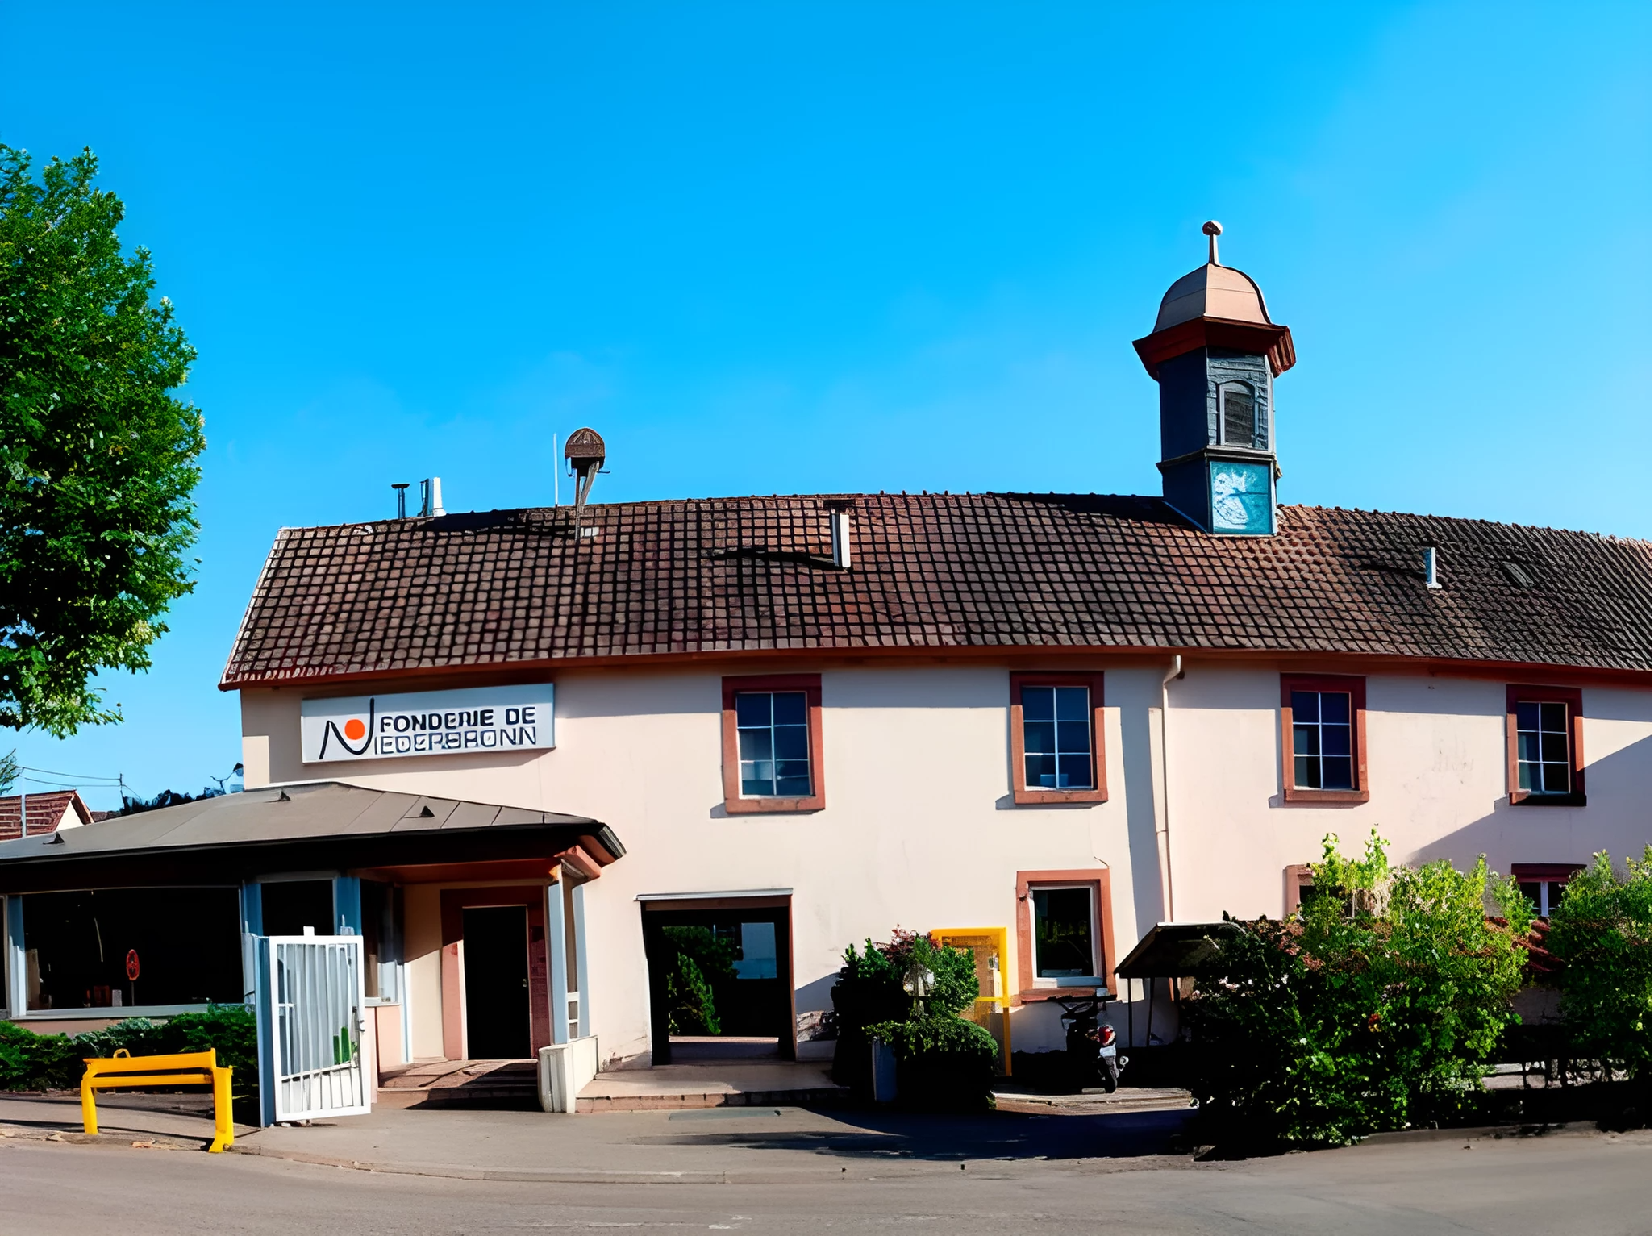
\includegraphics[scale=0.27]{Images/Presentation/Fonderie_vue_de_bas.pdf}
    \hspace{0.5 cm}
    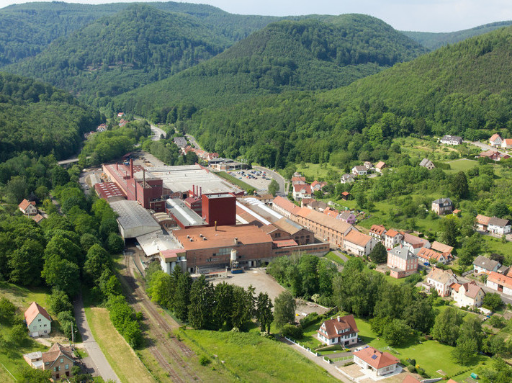
\includegraphics[scale=0.27]{Images/Presentation/Fonderie_vue_de_haut.pdf}
    \caption{Vues extérieure et aérienne de la Fonderie de Niederbronn}
\end{figure}

\newpage

\subsection{Description du processus de production des pièces en fonte}

La production de pièces en fonte suit un processus ordonnée et méticuleux, 
composé de plusieurs étapes interconnectées qui garantissent la qualité 
et la durabilité des produits finis. Chaque étape, depuis la préparation 
des matériaux jusqu'au produit final, est cruciale pour obtenir des pièces 
répondant aux exigences techniques et aux normes industrielles. 
Le schéma ci-dessous illustre ce flux de production, offrant une vue 
d'ensemble des différentes phases. 

\begin{figure}[H]
    \centering
    \begin{adjustbox}{width=1.3\textwidth,height=0.8\textheight,center}
        \includegraphics{Images/Presentation/Flux de production.pdf}
    \end{adjustbox}
    \caption{Flux de production des pièces en fonte.}
    \label{fig:flux-production}
\end{figure}


\begin{enumerate}
    \item \textbf{Chargement des matières premières :}
    À cette étape, les matériaux de base nécessaires à la production de la 
    fonte sont préparés. Ce processus comprend le tri, le nettoyage et la 
    sélection des matières premières, telles que le fer, le cuivre, les 
    déchets métalliques provenant d'autres industries, ainsi que des 
    alliages comme le magnésium et le silicium. Il est essentiel de choisir
    ces matériaux en fonction de leur composition chimique afin d'obtenir 
    les propriétés mécaniques souhaitées dans la fonte, car certains 
    éléments chimiques peuvent altérer la qualité du produit final.

    Voici une illustration des matières premières utilisées dans la fonderie :

    \begin{figure}[H]
        \centering
        \vfill
        \hspace{0.8 cm}
        \includegraphics[scale=0.7]{Images/Presentation/Les Retours.pdf}
        \hspace{0.5 cm}
        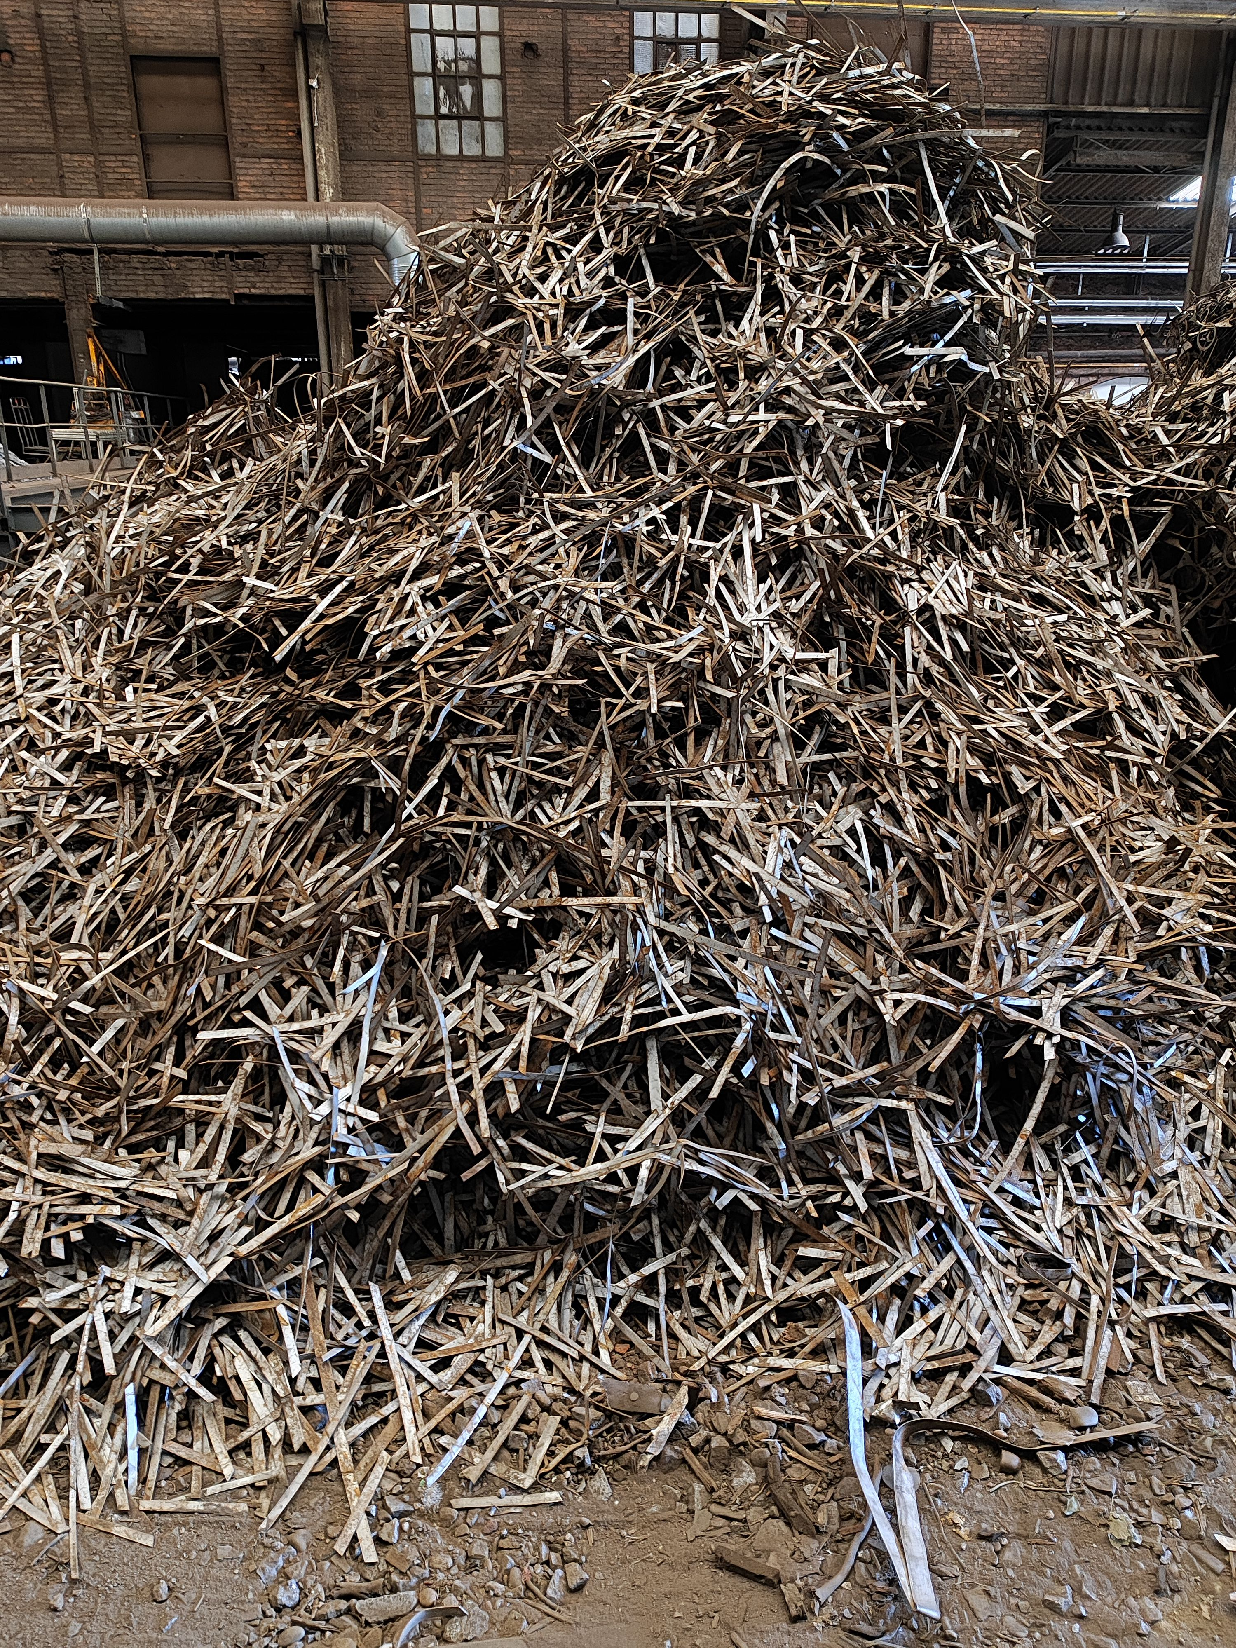
\includegraphics[scale=0.7]{Images/Presentation/Frite Haut Silicium.pdf}
        \caption{Les retours et les Frite Haut Silicium}
    \end{figure}

    \begin{figure}[H]
        \centering
        \vfill
        \hspace{0.8 cm}
        \includegraphics[scale=0.7]{Images/Presentation/Fontes d'affinages.pdf}
        \hspace{0.5 cm}
        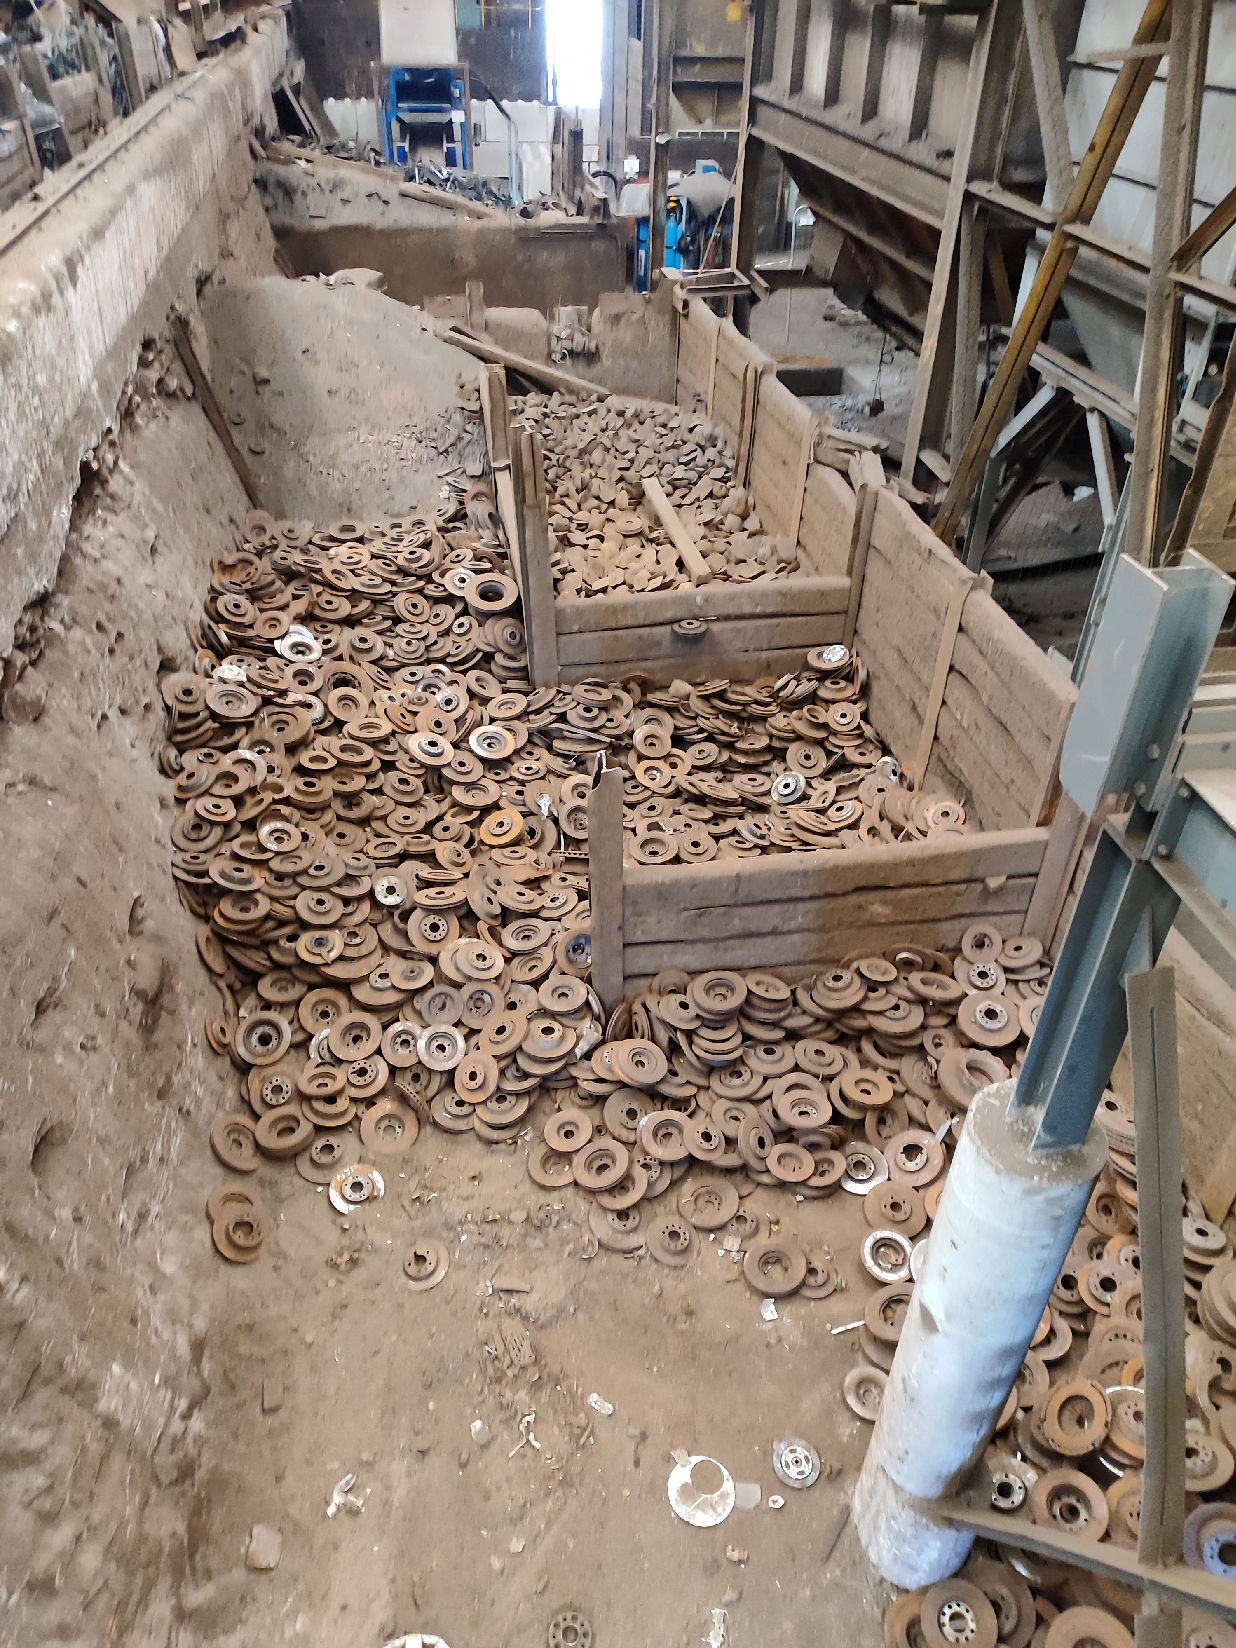
\includegraphics[scale=0.7]{Images/Presentation/Disque.pdf}
        \caption{Les Fontes d'affinages et les Disques}
    \end{figure}


    \item \textbf{Fusion :} Après la sélection des métaux, ceux-ci sont 
    fondus dans un four à induction qui atteint des températures 
    suffisamment élevées pour les transformer en métal liquide.

    \item \textbf{Modélage :} 
    Le modélage est l'une des premières étapes de la production en fonderie.
    Il consiste à préparer le modèle et le moule nécessaires pour la coulée.
    La pièce finale est d'abord conçue numériquement à l'aide de logiciels 
    de CAO. Une fois la conception validée, un modèle physique est fabriqué
    en métal.

    Le moule, généralement réalisé en sable mélangé à de l'argile et de 
    l'eau, est compacté autour du modèle. Le sable doit être suffisamment 
    résistant pour supporter le poids du métal fondu sans se désagréger. 
    Après compactage, le modèle est retiré et les parties du moule sont 
    assemblées. Des conduits de coulée sont ensuite ajoutés pour permettre 
    au métal fondu de remplir la cavité du moule.

    % ----------------- Mettre image de modèle physique ?!


    \item \textbf{Noyautage :} 
    Le noyautage constitue une étape importante dans le processus de 
    fabrication des pièces moulées, notamment pour créer des formes 
    internes complexes ou des cavités spécifiques. Semblables au moule, 
    les noyaux sont souvent réalisés en sable et façonnés à l'aide de 
    boîtes à noyaux qui leur confèrent la géométrie requise. Ces noyaux 
    jouent un rôle déterminant en permettant la formation de canaux et 
    d'autres détails internes indispensables à la pièce finale. 
    Une fois confectionnés, ils sont positionnés avec précision dans 
    le moule, où ils doivent être solidement fixés afin d'éviter 
    tout déplacement pendant la coulée.


    \item \textbf{Sphéroïdisation :} 
    Cette étape est spécifiquement dédiée aux fontes à graphite sphéroïdal 
    (fonte GS). La sphéroïdisation est un procédé essentiel visant à 
    optimiser les propriétés mécaniques de la fonte, en particulier sa 
    ductilité et sa résistance à la traction. Ce processus repose sur 
    l’ajout de magnésium à la fonte liquide, favorisant ainsi la formation 
    de graphite sous forme sphéroïdale plutôt que lamellaire. L'ajout de 
    magnésium se fait souvent à travers un alliage, tel que le fil fourré. 
    Cette transformation microstructurale, en remplaçant les lamelles de 
    graphite par des sphéroïdes, permet d'améliorer significativement les 
    performances mécaniques et la durabilité de la fonte, la rendant ainsi 
    plus adaptée aux applications exigeantes.


    % ----------------- Mettre image Microscopique de la fonte GS

    \item \textbf{Inoculation et Dégrassage :} Dans cette étape, des agents d'inoculation sont 
    ajoutés au métal fondu pour contrôler la structure et les propriétés finales de 
    la fonte GS. Ces agents favorisent la formation de sphéroïdes de graphite de 
    taille et de forme uniformes.

    L'inoculation est réalisée après la sphéroïdisation pour contrôler la structure 
    et les propriétés finales de la fonte. Des agents inoculants, tels que le 
    ferrosilicium, sont ajoutés pour favoriser une précipitation uniforme et fine 
    du graphite.

    Le Degrassage consiste  à enlever la grasse dans la fonte

    % ----------------- Mettre image Innoculation/Degrassange en action ou du produits innoculant
    
    \item \textbf{Moulage ou Coulée :} La fonte est  versé dans 
    le moule à travers les conduits de coulée pour prendre la forme finale de la pièce. Une 
    fois coulé, le métal liquide refroidit et se solidifie à l'intérieur du moule, prenant la 
    forme de la cavité créée par le modèle et les noyaux.



    \item \textbf{Décochage et Grenaillage :} 

    Après la coulée, Une fois le métal solidifié, le moule est démonté pour extraire 
    la pièce coulée. Les moules en sable sont souvent détruits au cours de ce processus,
    tandis que les moules permanents peuvent être réutilisés. Les noyaux en sable sont 
    retirés, souvent à l'aide de vibrations ou de lavage, pour révéler les cavités 
    internes de la pièce. Grenaillage : La pièce est ensuite nettoyée par projection 
    de billes d'acier (ou d'autres matériaux abrasifs) pour enlever la calamine, les 
    restes de sable et améliorer la surface.
    
    \item \textbf{Ebarbage et Usinage :} 
    La pièce obtenue après démoulage n'est pas encore prête pour une utilisation directe. 
    Elle doit subir plusieurs opérations de finition. Les pièces sont ébarbées pour 
    enlever les bavures et les excès de métal laissés par les joints du moule ou les 
    conduits de coulée. Les pièces peuvent être usinées pour atteindre des dimensions 
    précises et une surface lisse.
    

    \item \textbf{Peinture :} La peinture et le revêtement sont appliqués à la pièce 
    pour la protéger de la corrosion et lui donner un aspect esthétique. La surface de 
    la pièce est nettoyée et préparée pour une meilleure adhérence de la peinture.
    Des peintures ou des revêtements spécifiques sont appliqués par pulvérisation, 
    trempage ou brossage.



    \item \textbf{Contrôle qualité et Livraison :} Avant la livraison des pièces finales, un 
    contrôle qualité est effectué pour s'assurer qu'elles répondent aux normes et 
    aux spécifications requises. La composition chimique de la pièce est analysée pour 
    s'assurer qu'elle correspond aux spécifications. Des tests de traction, de dureté, 
    et d'impact peuvent être effectués pour valider les propriétés mécaniques de la 
    pièce.
\end{enumerate}



\subsection{L'objectif du stage }


% Presenter rapidement L'objectif du stage
L’objectif principal de ce stage est d’optimiser l’utilisation des matières 
premières recyclées dans la production de fonte à hautes caractéristiques 
mécaniques. Le projet s’inscrit dans le cadre d’un crédit d’impôt recherche 
et vise à modéliser et automatiser les processus liés au choix et aux 
quantités des différentes matières premières. Voici les missions confiées :

\begin{itemize}
    \item Modéliser le système via des équations.
    \item Contribuer à l’optimisation des coûts de revient en 
    automatisant les processus.
    \item Participer à d’autres sujets d’optimisation en parallèle.
\end{itemize}


\subsection{Le plan du rapport}

% Presenter rapidement le plan du rapport
Le présent rapport couvre les éléments suivants : la présentation de 
la fonderie de Niederbronn, la description du processus 
de production et de l'objectif du stage, 

mandat du stage la méthodologie utilisée durant le stage, et les résultats du stage. En
fin une conclusion boucle ce rapport de stage.



%---- motiver le sujet et objectif stage


%---- détail objectif stage





\section{L'étude statistique}

% Contexte et Objectifs

\subsection{Contexte et Objectifs}

Nous disposons de 2 mesures normatives la résistance mécanique en MPA et l'allongement 
en pourcentage , de la composition chimique de la fonte étudiée obtenus grâce au 
spectromètre et de 5 indicateurs de qualités, qui sont des combinaisons d'éléments 
chimiques.
L'objectif est d'évaluer la pertinance des 5 indicateurs de qualités à la vue 
des 2 mesures normatives et de sélectionner  les meilleurs indicateurs de qualité 
et donner leurs intervalle de prédictions.


\subsection{Les données}

% Source des données

Les données utilisées dans ce projet proviennent de deux sources principales :
une machine de Traction et d'un Spectromètre . 
D'aborb, la résistance mécanique et l'allongement sont mesurées à l'aide d'une 
machine de traction. Ensuite, Les données concernant les éléments chimiques dans 
la fonte sont obtenus à l'aide de spectromètres.


% Format des données

Les données sont au format Données au format Windev extraites dans un fichier Excel.
Le Type de Données est la Base de données. Nous disposons d'une de données et de features .

La Figure ci-dessous ~\ref{fig:donnees_brutes}  illustre l'état initial des données avant tout 
processus de nettoyage ou d'analyse.


% Les données brutes
\begin{figure}[H]
    \centering
    \adjustbox{width=1.23\textwidth, center}{
        \begin{minipage}{\textwidth}
            \centering
            \includegraphics[width=0.75\paperwidth]{Images/Statistique/DonnéesBrut1.pdf} \\
            \vspace{25pt}
            \includegraphics[width=0.75\paperwidth]{Images/Statistique/DonnéesBrut2.pdf} \\
            \vspace{25pt}
            \includegraphics[width=0.75\paperwidth]{Images/Statistique/DonnéesBrut3.pdf}
        \end{minipage}
    }
    \caption{Visualisation des données brutes}
    \label{fig:donnees_brutes}
\end{figure}



    
    
% Description des données


\textbf{Les variables quantitatives :}

\begin{itemize}
\item Rm : Résistance mécanique à la traction.
\item Rp0.2 : Limite d'élasticité à 0,2% de déformation.
\item A\% : Allongement à la rupture en pourcentage.
\item Contre-essai A\% : Contre-essai de l'allongement à la rupture en pourcentage.
\item Moyenne allongement : Moyenne de l'allongement à la rupture en pourcentage.
\end{itemize}
    

\textbf{Les indicateurs :}

\begin{itemize}
\item Impureté : Pourcentage d'impureté dans l'échantillon.
\item \% Ferrite : Pourcentage de ferrite dans l'échantillon.
\item ONO, TANIMURA, ... : Un indicateur de qualité en pourcentage.
\item THIELMANN : Un indicateur de qualité en pourcentage.
\end{itemize}
 

\textbf{Les variables qualitatives :}

\begin{itemize}
\item Recette : Nom ou code de la recette associée à l'échantillon.
\item Date : Date à laquelle la coulée a été effectuée.
\item Poche/Four/Barreau : Indication sur la provenance de l'échantillon (poche, four, barreau, etc.).
\item Conforme ? : Indique si l'échantillon est conforme (1) ou non conforme (0) aux critères définis.
\item Pièces : Référence des pièces.
\item Observations : Commentaires ou observations sur l'échantillon.
\item Comment. RQ : Commentaires ou remarques supplémentaires.
\end{itemize}

\textbf{Les éléments chimiques :}

\begin{itemize}
\item C, Si, Mn, P, Cr, Mo, Cu, Sn, Mg, Ce, Ca, Al 
\item Zn, Ti, S, Sn, V, Pb, Al, Bi, B, Te, Sb, As, Ti 
\end{itemize}



% Prétraitement des Données


Avant d'utiliser les données dans l'étude, elles ont été soumises aux prétraitements suivants :

\begin{itemize}
\item Nettoyage des données :
\begin{itemize}
\item Suppression des colonnes : Date, Rp0.2, A\%, Contre-essai A\%, Pièces, Observations, Comment. RQ, PJ, Ca, Ba.
\item Suppression des lignes incomplètes (celles avec des colonnes vides).
\end{itemize}
\item Ajout de l'indicateur Pureté MAYER.
\item Mise en forme des données :
\begin{itemize}
\item Renommage des colonnes.
\item Séparation des données en fonction  du type de recette.
\item Séparation des données en fonction de la conformité de l'échantillon.
\end{itemize}
\end{itemize}
    


% Les données nettoyées
\begin{figure}[H]
    \centering
    \adjustbox{width=1.3\textwidth, center}{
        \begin{minipage}{\textwidth}
            \centering
            \includegraphics[width=\textwidth]{Images/Statistique/DonnéesClean1.pdf} \\
            \vspace{25pt}
            \includegraphics[width=\textwidth]{Images/Statistique/DonnéesClean2.pdf}
        \end{minipage}
    }
    \caption{Visualisation des données nettoyées}
    \label{fig:donnees_nettoyees}
\end{figure}


\subsection{Les indicateurs}



% Les indicateurs


\begin{itemize}
  \item  Evaluer la pertinence des cinq indicateurs de qualité à la vue des deux mesures normatives.
  \item Dans le but d'évaluer l'influence globale des différents éléments sur la matrice ou la forme du graphite, plusieurs formules ont été proposées par divers auteurs.
\end{itemize}

Voici les 5 formules, qui consistent en une somme pondérée des éléments chimiques :




\begin{align*}
    \textcolor{blue}{\text{Pureté MAYER \%}} &= \text{Ti\%} + \text{Pb\%} + \text{Bi\%} + \text{Sb\%} \\
    \textcolor{red}{\text{Ferrite \%}} &= 92.3 - 96.2 (\text{Mn \%}) - 211 (\text{Cu \%}) - 14270 (\text{Pb \%}) \\
    &\quad - 2815 (\text{Sb \%}) \\
    \textcolor{green}{\text{Pureté ONO \%}} &= \text{Cu \%} + \text{Ti \%} + \text{Ni \%} + \text{Cr \%} + \text{V \%} + \text{Al \%} + \text{As \%} \\
    &\quad + \text{Sn \%} + \text{Pb \%} + \text{Sb \%} + \text{Bi \%} \\
    \textcolor{purple}{\text{Impureté \%}} &= 4.9 (\text{Cu \%}) + 0.37 (\text{Ni \%}) + 0.37 (\text{Cr \%}) + 7.9 (\text{Mo \%}) \\
    &\quad + 4.4 (\text{Ti \%}) + 39.0 (\text{Sn \%}) + 0.44 (\text{Mn \%}) + 5.6 (\text{P \%}) \\
    \textcolor{orange}{\text{Pureté THIELMANN \%}} &= 4.4 (\text{Ti \%}) + 2.0 (\text{As \%}) + 2.3 (\text{Sn \%}) + 5.0 (\text{Sb \%}) \\
    &\quad + 290 (\text{Pb \%}) + 370 (\text{Bi \%}) + 1.6 (\text{Al \%})
\end{align*}
    
   
% \begin{align*}
%     \textcolor{blue}{\text{Pureté MAYER \%}} &= \text{Ti\%} + \text{Pb\%} + \text{Bi\%} + \text{Sb\%} \\
%     \textcolor{red}{\text{Ferrite \%}} &= 92.3 - 96.2 (\text{Mn \%}) - 211 (\text{Cu \%}) - 14270 (\text{Pb \%}) - 2815 (\text{Sb \%})\\
%     \textcolor{green}{\text{Pureté ONO \%}} &= \text{Cu \%} + \text{Ti \%} + \text{Ni \%} + \text{Cr \%} + \text{V \%} + \text{Al \%} + \text{As \%} + \text{Sn \%} \\
%     &\quad + \text{Pb \%} + \text{Sb \%} + \text{Bi \%} \\
%     \textcolor{purple}{\text{Impureté \%}} &= 4.9 (\text{Cu \%}) + 0.37 (\text{Ni \%}) + 0.37 (\text{Cr \%}) + 7.9 (\text{Mo \%}) + 4.4 (\text{Ti \%}) \\
%     &\quad + 39.0 (\text{Sn \%}) + 0.44 (\text{Mn \%}) + 5.6 (\text{P \%}) \\
%     \textcolor{orange}{\text{Pureté THIELMANN \%}} &= 4.4 (\text{Ti \%}) + 2.0 (\text{As \%}) + 2.3 (\text{Sn \%}) + 5.0 (\text{Sb \%}) + 290 (\text{Pb \%}) \\
%     &\quad + 370 (\text{Bi \%}) + 1.6 (\text{Al \%})
% \end{align*}
    
    



% Voici la méthode utiliser  pour les classsememt sur la plus grande valeur de (|Rm| + |Allongement|)/2

% La corrélation de Pearson


Pour évaluer nos indicateurs, nous utilisons la corrélation de Pearson afin de quantifier la relation linéaire entre ces derniers et les mesures d'allongement et de résistance mécanique.

\vspace{10pt}
Les étapes de l'évaluation sont les suivantes :
\vspace{5pt}

\begin{enumerate}
\item Calcul des coefficients de corrélation.
\item Classement des indicateurs en fonction de leur corrélation avec l'allongement et la résistance mécanique.
\item Conservation des indicateurs présentant la dépendance linéaire la plus significative avec les deux mesures normatives.
\end{enumerate}



% Évaluation des indicateurs 

\textbf{Corrélation entre les indicateurs et les mesures normatives} 
\begin{figure}[H]
    \includegraphics[width=\textwidth]{Images/Statistique/Matrice_corrélation_qualite_indicateur.pdf} 
\end{figure}


\textbf{ Classement des indicateurs :}
\begin{itemize}
    \item Impureté [\%] : 0.673506
    \item Pureté ONO [\%] : 0.583101
    \item Pureté THIELMANN [\%] : 0.353988
    \item Pureté MAYER [\%] : 0.346637
    \item Ferrite [\%] : 0.327601
\end{itemize}


La matrice de corrélations fournit des informations précieuses sur les relations entre différentes variables de notre jeu de données. Ces corrélations peuvent non seulement aider à prédire une variable en fonction d'une autre, mais aussi à comprendre les interactions et les influences entre les variables. Voici les principales observations :

Une forte corrélation positive (0.65) a été observée entre “Rm [MPa]” et “Moyenne alignement [\%]”. Cela indique que lorsque la résistance à la traction (Rm) augmente, la moyenne d'alignement a également tendance à augmenter.
De même, une forte corrélation positive (0.62) entre “Rm [MPa]” et “Purete ONO [\%]” montre que l'augmentation de la pureté ONO est généralement associée à une résistance à la traction plus élevée.

Une très forte corrélation positive (0.86) a été identifiée entre “Moyenne alignement [\%]” et “Ferrite [\%]”. Cette relation suggère que les niveaux de ferrite augmentent parallèlement à l'amélioration de l'alignement moyen, ce qui pourrait indiquer des mécanismes sous-jacents communs influençant ces deux variables.
Une corrélation négative (-0.41) entre “Rm [MPa]” et “Ferrite [\%]” indique que des niveaux plus élevés de ferrite sont associés à une diminution de la résistance à la traction. Cela pourrait impliquer que la présence de ferrite a un effet affaiblissant sur le matériau.

Une corrélation négative notable (-0.52) entre “Rm [MPa]” et “Purete THIELMANN [\%]” suggère qu'une pureté THIELMANN plus élevée est liée à une réduction de la résistance à la traction.




\subsection{Les éléments chimiques}



%  Les éléments chimiques

Examinons de près les éléments chimiques qui composent l'impureté, la pureté ONO et le taux de ferrite.

Selon la littérature, on classe les éléments chimiques en plusieurs catégories :

\begin{itemize}
    \item \textbf{Les éléments d'alliage :}  C, Si, Mn, P, Cr, Mo, Cu, Sn 
    \item \textbf{Les éléments de traitement :} Mg, Ce, Ca, Al
    \item \textbf{Les éléments polluants :}  Zn, Ti, S, Sn, V 
    \item \textbf{Les éléments poisons :}  Pb, Al, Bi, B, Te, Sb, As, Ti
\end{itemize}
\vspace{5pt}
Dans la formule de la pureté ONO, on retrouve les 4 types d'éléments.
Quant à l'impureté, elle quantifie des éléments poisons, des éléments polluants et des éléments d'alliage.



% Impureté

\textbf{Corrélation entre l'impureté et les éléments chimiques} 

\begin{figure}[H]
    \includegraphics[width=\textwidth]{Images/Statistique/Matrice_corrélation_Impurete_Elements.pdf} 
\end{figure}

\textbf{Classement des éléments chimiques :}
\begin{itemize}
    \item Sn (Étain) [\%] : 0.902219
    \item Cu (Cuivre) [\%] : 0.753903
    \item Cr (Chrome) [\%] : 0.522274
\end{itemize}


Une forte corrélation positive (0.88) est observée entre le Chrome (Cr) et le Molybdène (Mo). 
Les impuretés montrent une corrélation modérément positive avec le Nickel (Ni) et le Titane (Ti), toutes deux à 0.36. Cela indique que les niveaux de ces impuretés ont tendance à augmenter modérément lorsque la concentration de Ni ou de Ti augmente.
Les corrélations entre les impuretés et des éléments tels que le Cuivre (Cu), le Manganèse (Mn), et le Phosphore (P) sont faibles, avec des valeurs proches de 0. Cela suggère qu'il n'y a pas de relation significative entre ces éléments et les impuretés dans le contexte étudié.

% Purete ONO


\textbf{Corrélation entre la purete ONO et les éléments chimiques}
\begin{figure}[H]
    \includegraphics[width=\textwidth]{Images/Statistique/Matrice_corrélation_ONO_Elements.pdf} 
\end{figure}

\textbf{Classement des éléments chimiques : }
\begin{itemize}
    \item Cu (Cuivre) [\%] : 0.934031
    \item Cr (Chrome) [\%] : 0.707962
    \item Sn (Étain) [\%] : 0.606912
    \item Ni (Nickel) [\%] : 0.590721
    \item V (Vanadium) [\%] : 0.527861
\end{itemize}

La pureté ONO [%] a une forte corrélation positive avec Cu [%] (0.93) et Ti [%] (0.92).
Il y a des corrélations positives modérées avec Ni [%] (0.59) et Cr [%] (0.53)
Les éléments comme Sb [%], Bi [%], et Al [%] montrent des corrélations faibles ou négligeables avec la pureté ONO, suggérant qu’ils n’ont pas un impact significatif sur celle-ci.
















% Conclusion de la partie corrélation

% Rajoute un texte à ce niveau

\textbf{Les indicateurs les plus pertinants}
\begin{itemize}
\item Impureté : 0.673506
\item Pureté ONO : 0.583101
\end{itemize}

\textbf{Les éléments chimiques conservés}
\begin{itemize}
\item Sn (Étain) 
\item Cu (Cuivre)
\item Cr (Chrome) 
\item V (Vanadium)
\end{itemize}






\subsection{Les valeurs extrêmes}

% Gestions des valeurs extrèmes


Pour améliorer la performance de la régression linéaire, nous procédons à la suppression des valeurs extrêmes basées sur les mesures d'impureté, de pureté ONO et de taux de ferrite. Voici la procédure suivie :

\begin{itemize}
    \item \textbf{Objectif} : Réduire la variabilité des données pour une meilleure performance de la régression linéaire.
    \item \textbf{Critère de suppression } : Une valeur est considérée comme extrême si elle se situe en dehors de l'intervalle défini par $[\bar{x} - 1.5(Q_3 - Q_1), \bar{x} + 1.5(Q_3 - Q_1)]$, où $Q_1$ et $Q_3$, le premier et le troisième quartile de la distribution des données, et $\bar{x}$ la moyenne des données.
    \item Cette suppression est réalisée de manière itérative jusqu'à ce qu'il n'y ait plus de valeurs extrêmes dans l'ensemble de données.
\end{itemize}



% Les valeurs extrèmes de l'impureté
\begin{figure}[H]
    \centering
    \begin{adjustbox}{width=1.3\textwidth,center}
        \includegraphics[scale=1]{Images/Statistique/Impureté_sans_extreme.pdf}
        \includegraphics[scale=1]{Images/Statistique/Impureté_avec_extreme.pdf}
    \end{adjustbox}
    \caption{L'impureté avant et après le traitement des valeurs extrèmes.}
    \label{fig:ExtremeImputerete}
\end{figure}


% Les valeurs extrèmes de ONO
\begin{figure}[H]
    \centering
    \begin{adjustbox}{width=1.3\textwidth,center}
        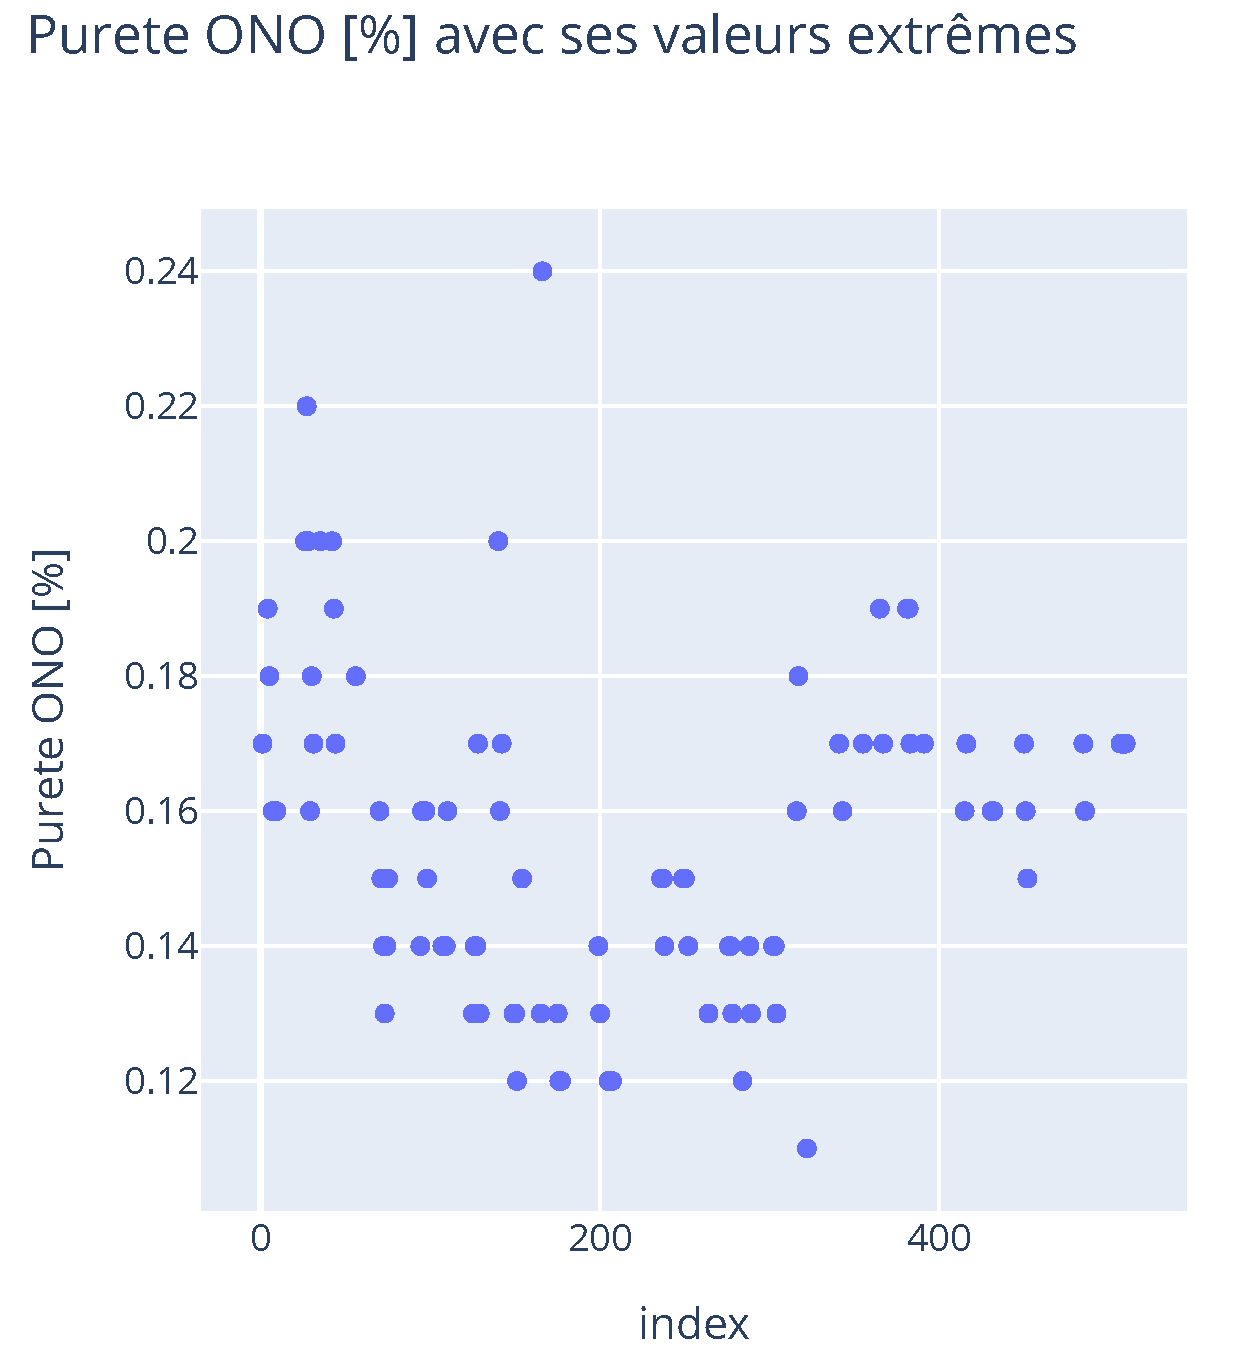
\includegraphics[scale=1]{Images/Statistique/Purete ONO_avec_extreme.pdf}
        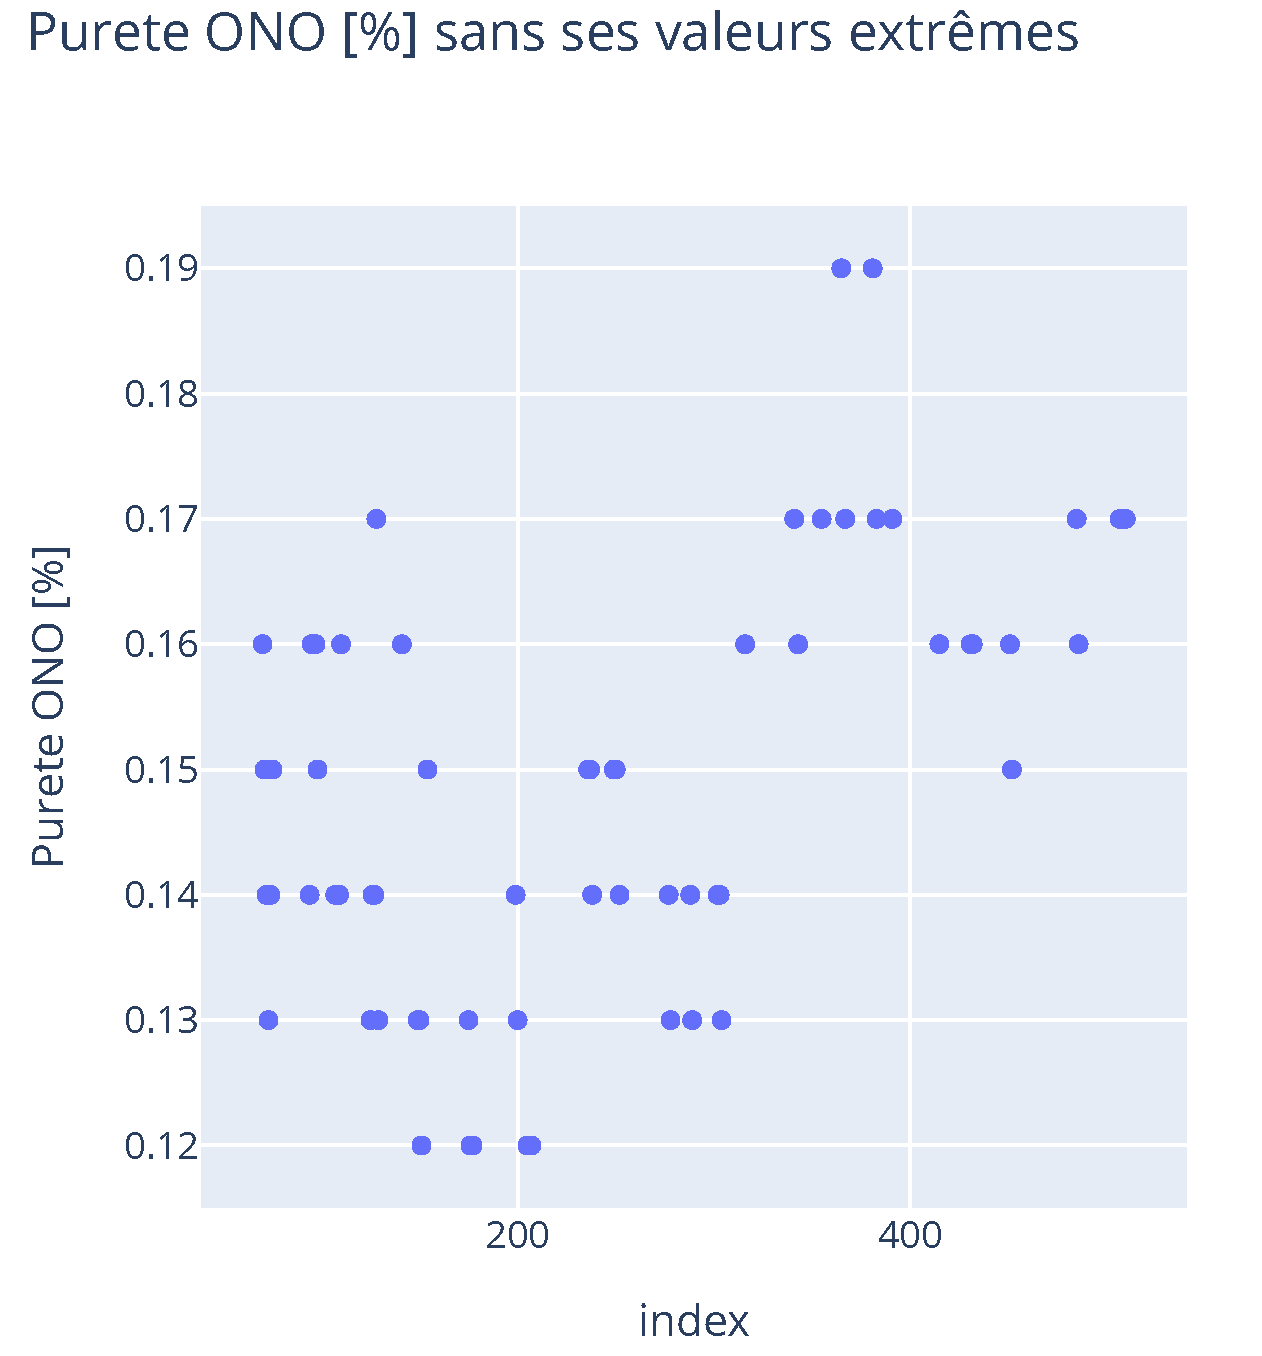
\includegraphics[scale=1]{Images/Statistique/Purete ONO_sans_extreme.pdf}
    \end{adjustbox}
    \caption{La purete ONO avant et après le traitement des valeurs extrèmes.}
    \label{fig:ExtremeONO}
\end{figure}

On peut alors discuter des bornes mininum et maximal de l'impurété et de ONO,
qui permet de garantir un bon lit de fusion.

Les données sont assez distantes l'une des autres, ce qui n'est pas idéal pour
avoir un intervale de confiance et de prediction fine


\subsection{La régression linéaire }

% La régression linéaire: Analyse des Données

Effectuons une régression linéaire et calculons les intervalles de  prédictions 
suivant les éléments chimiques et les indicateurs les plus pertinants.


\medskip % Mettre un espace

La formule des intervalles de prédiction est donnée par :
$$
IP (y_{pred}) = [y_{pred} - n \cdot predict\_se, y_{pred} + n \cdot predict\_se]
$$
Où :
\begin{itemize}
    \item $y_{pred}$ est la valeur prédite.
    \item predict\_se est  l'écart-type de prédiction.
    \item  n  est un entier naturel.
\end{itemize}






% % Regression linéaire entre Impurete et Sn, Cu
% \begin{figure}[H]
%     \centering
%     \begin{adjustbox}{width=1.35\textwidth,center}
%         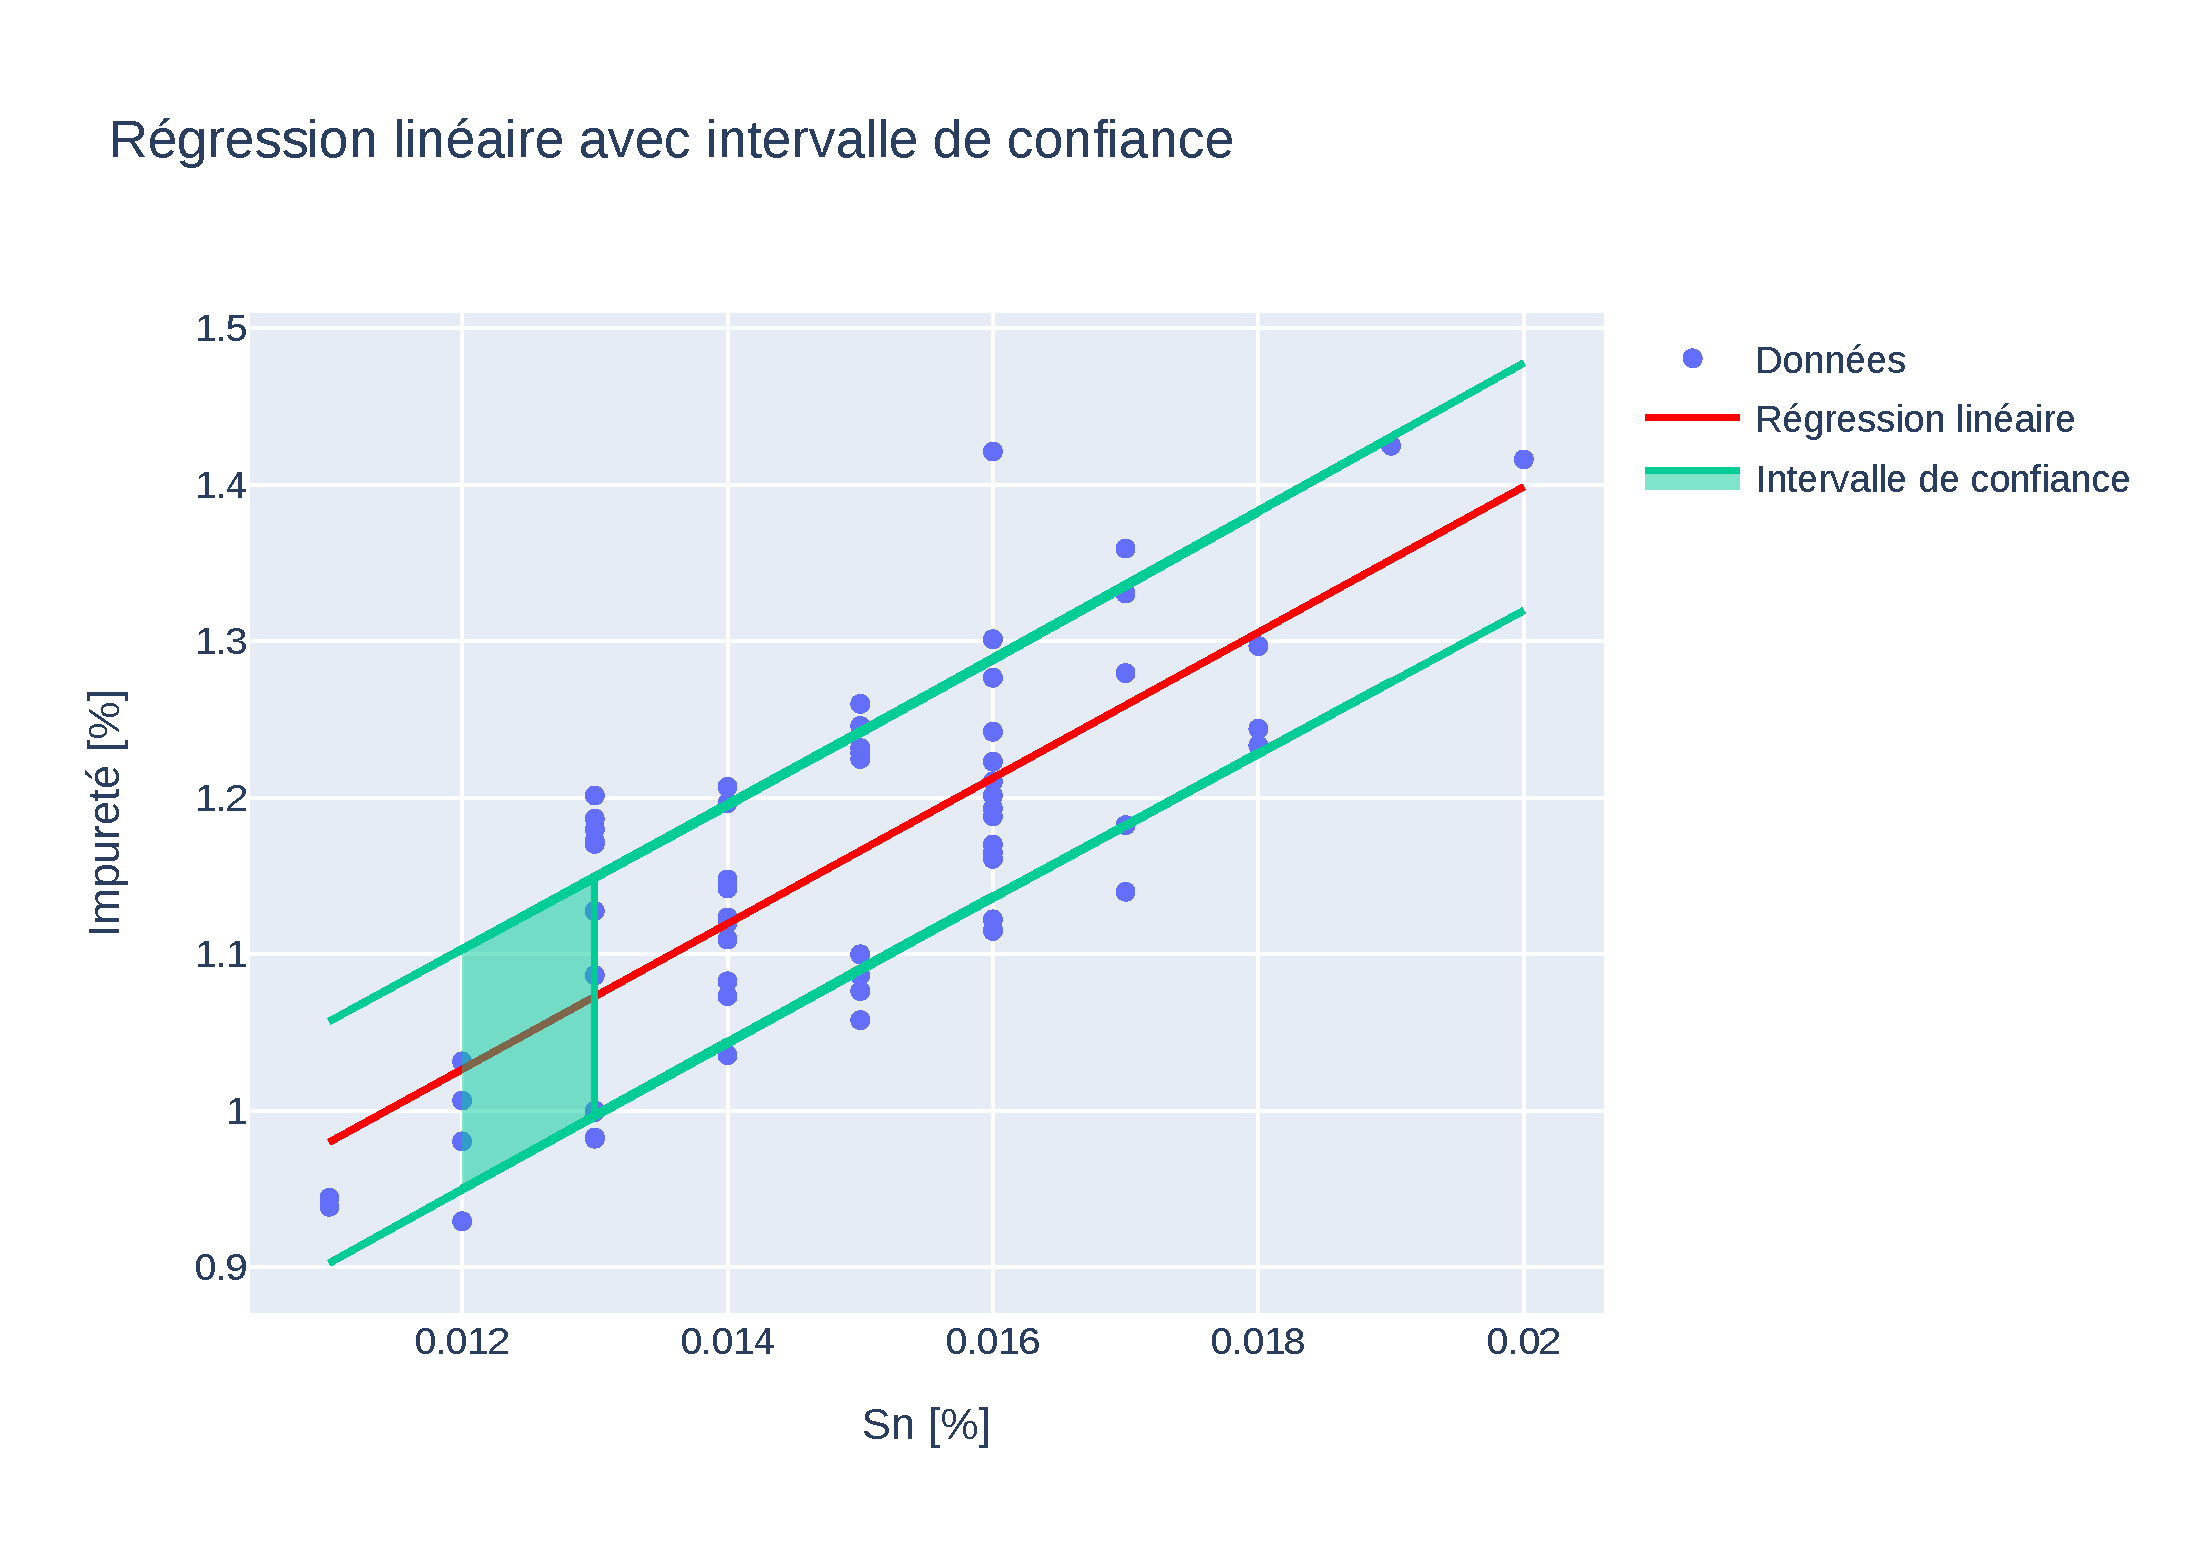
\includegraphics[scale=1]{Images/Statistique/Regression_Impurete_Sn.pdf}
%         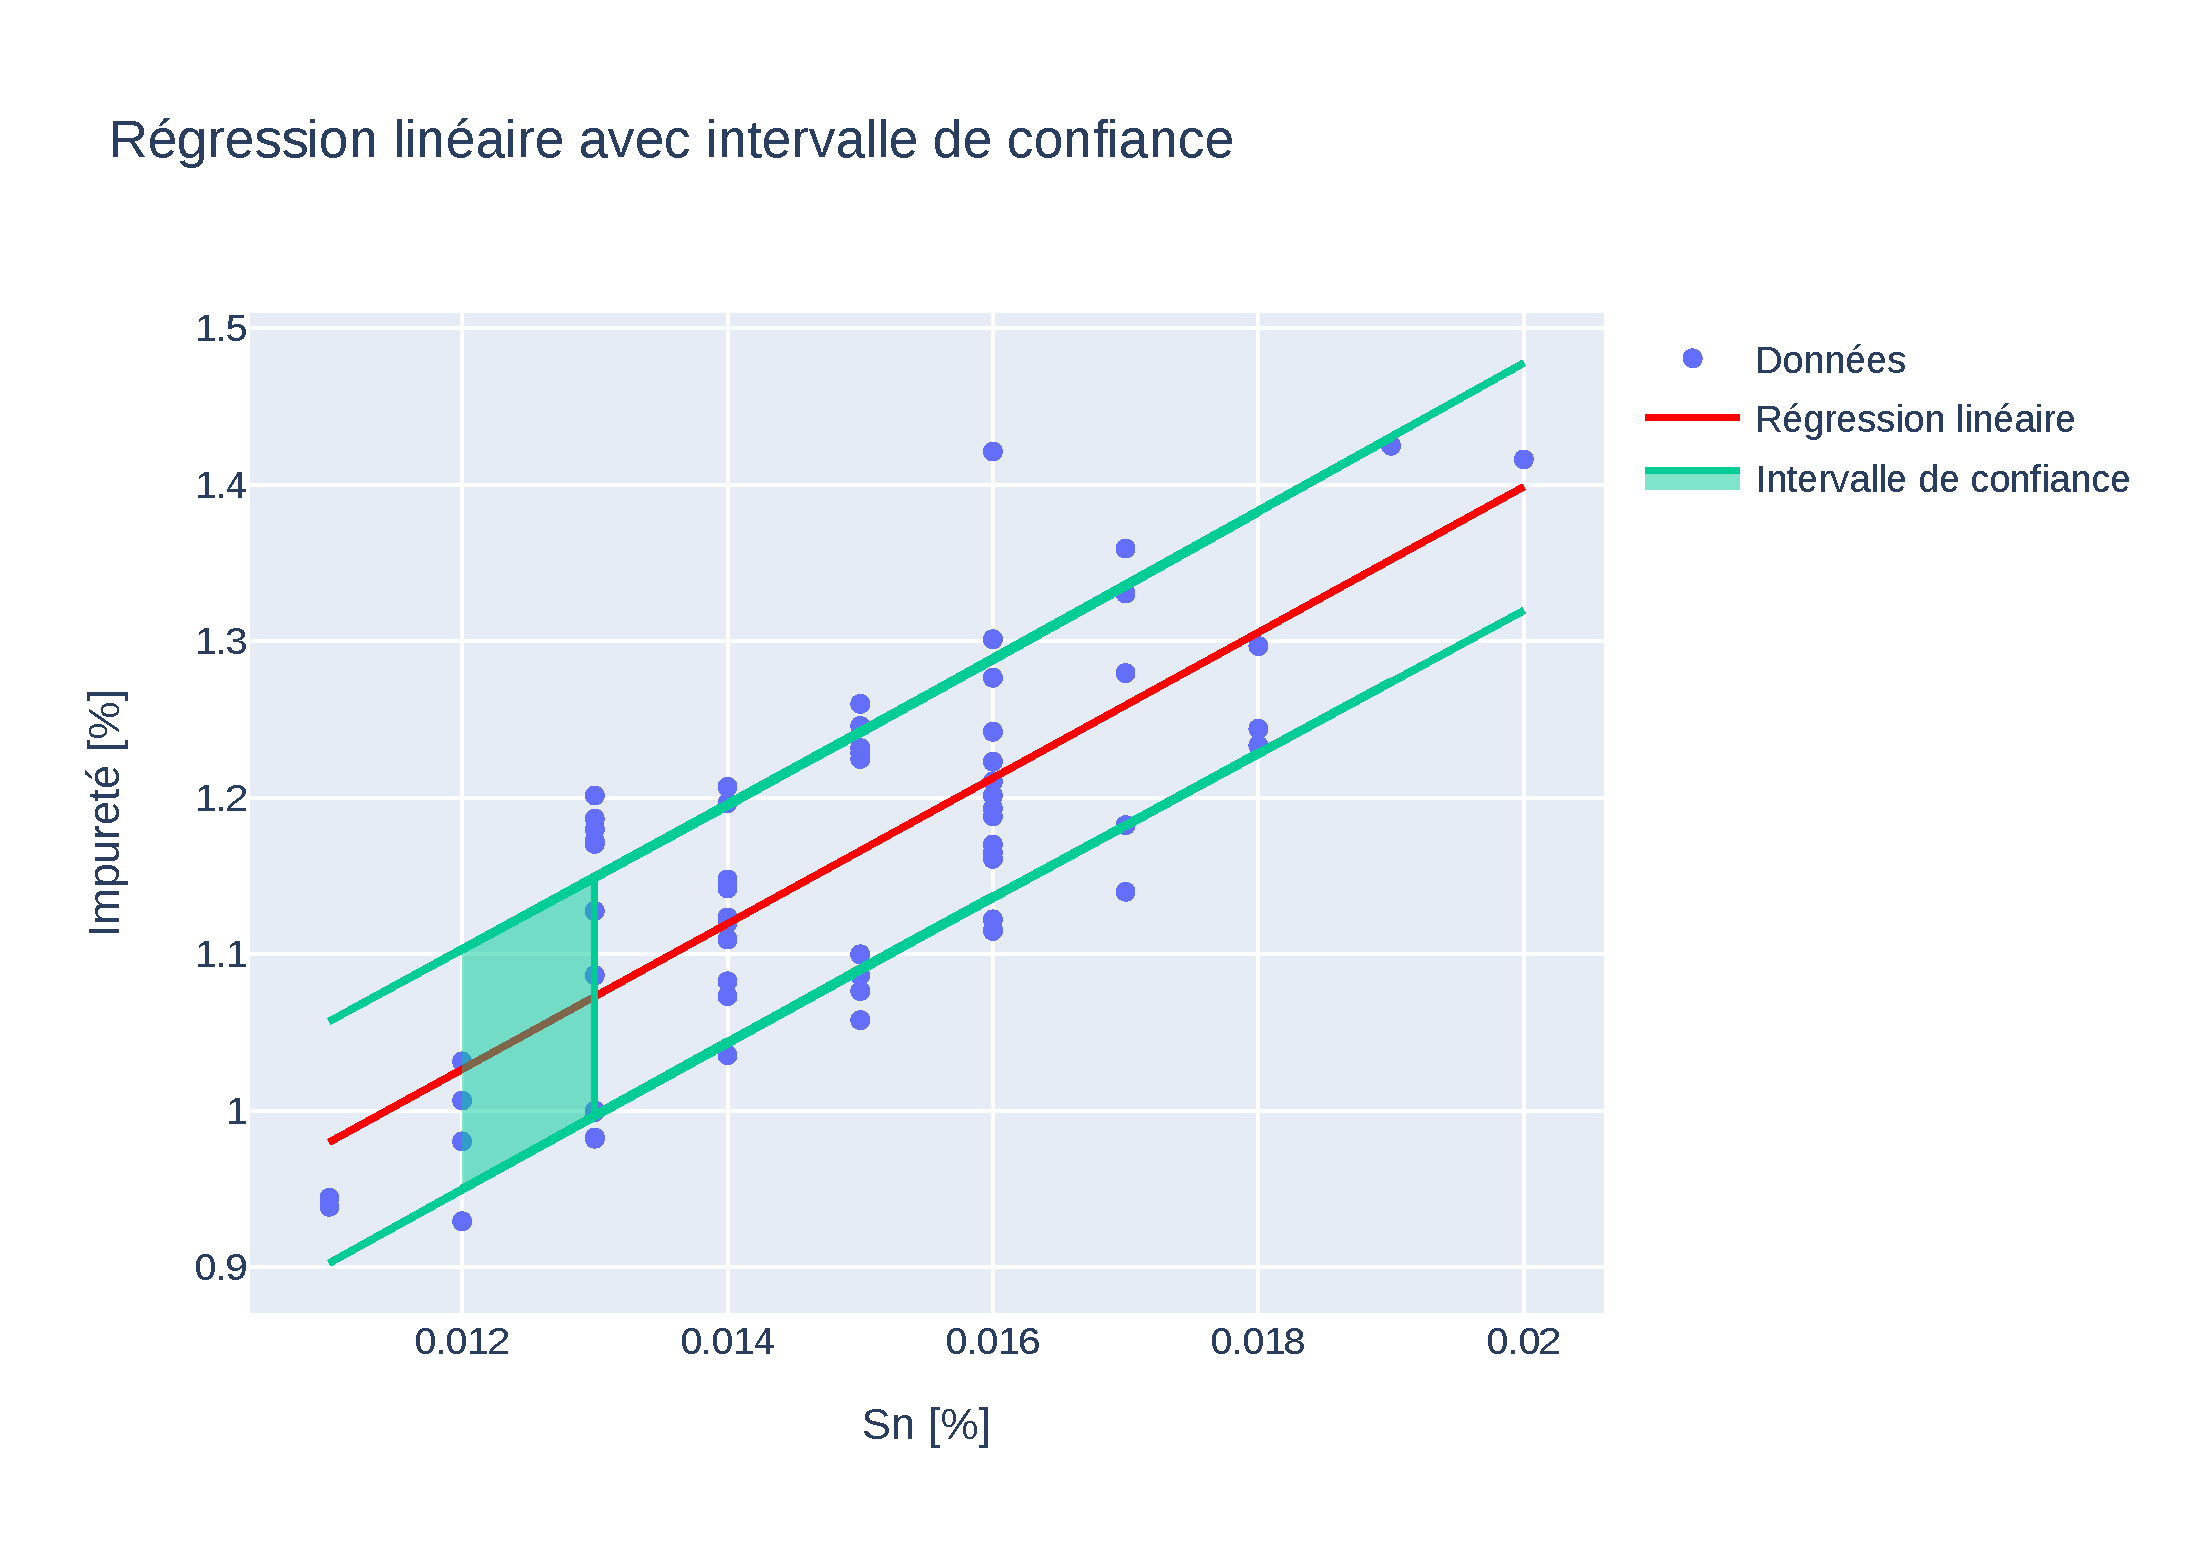
\includegraphics[scale=1]{Images/Statistique/Regression_Impurete_Sn.pdf}
%         % 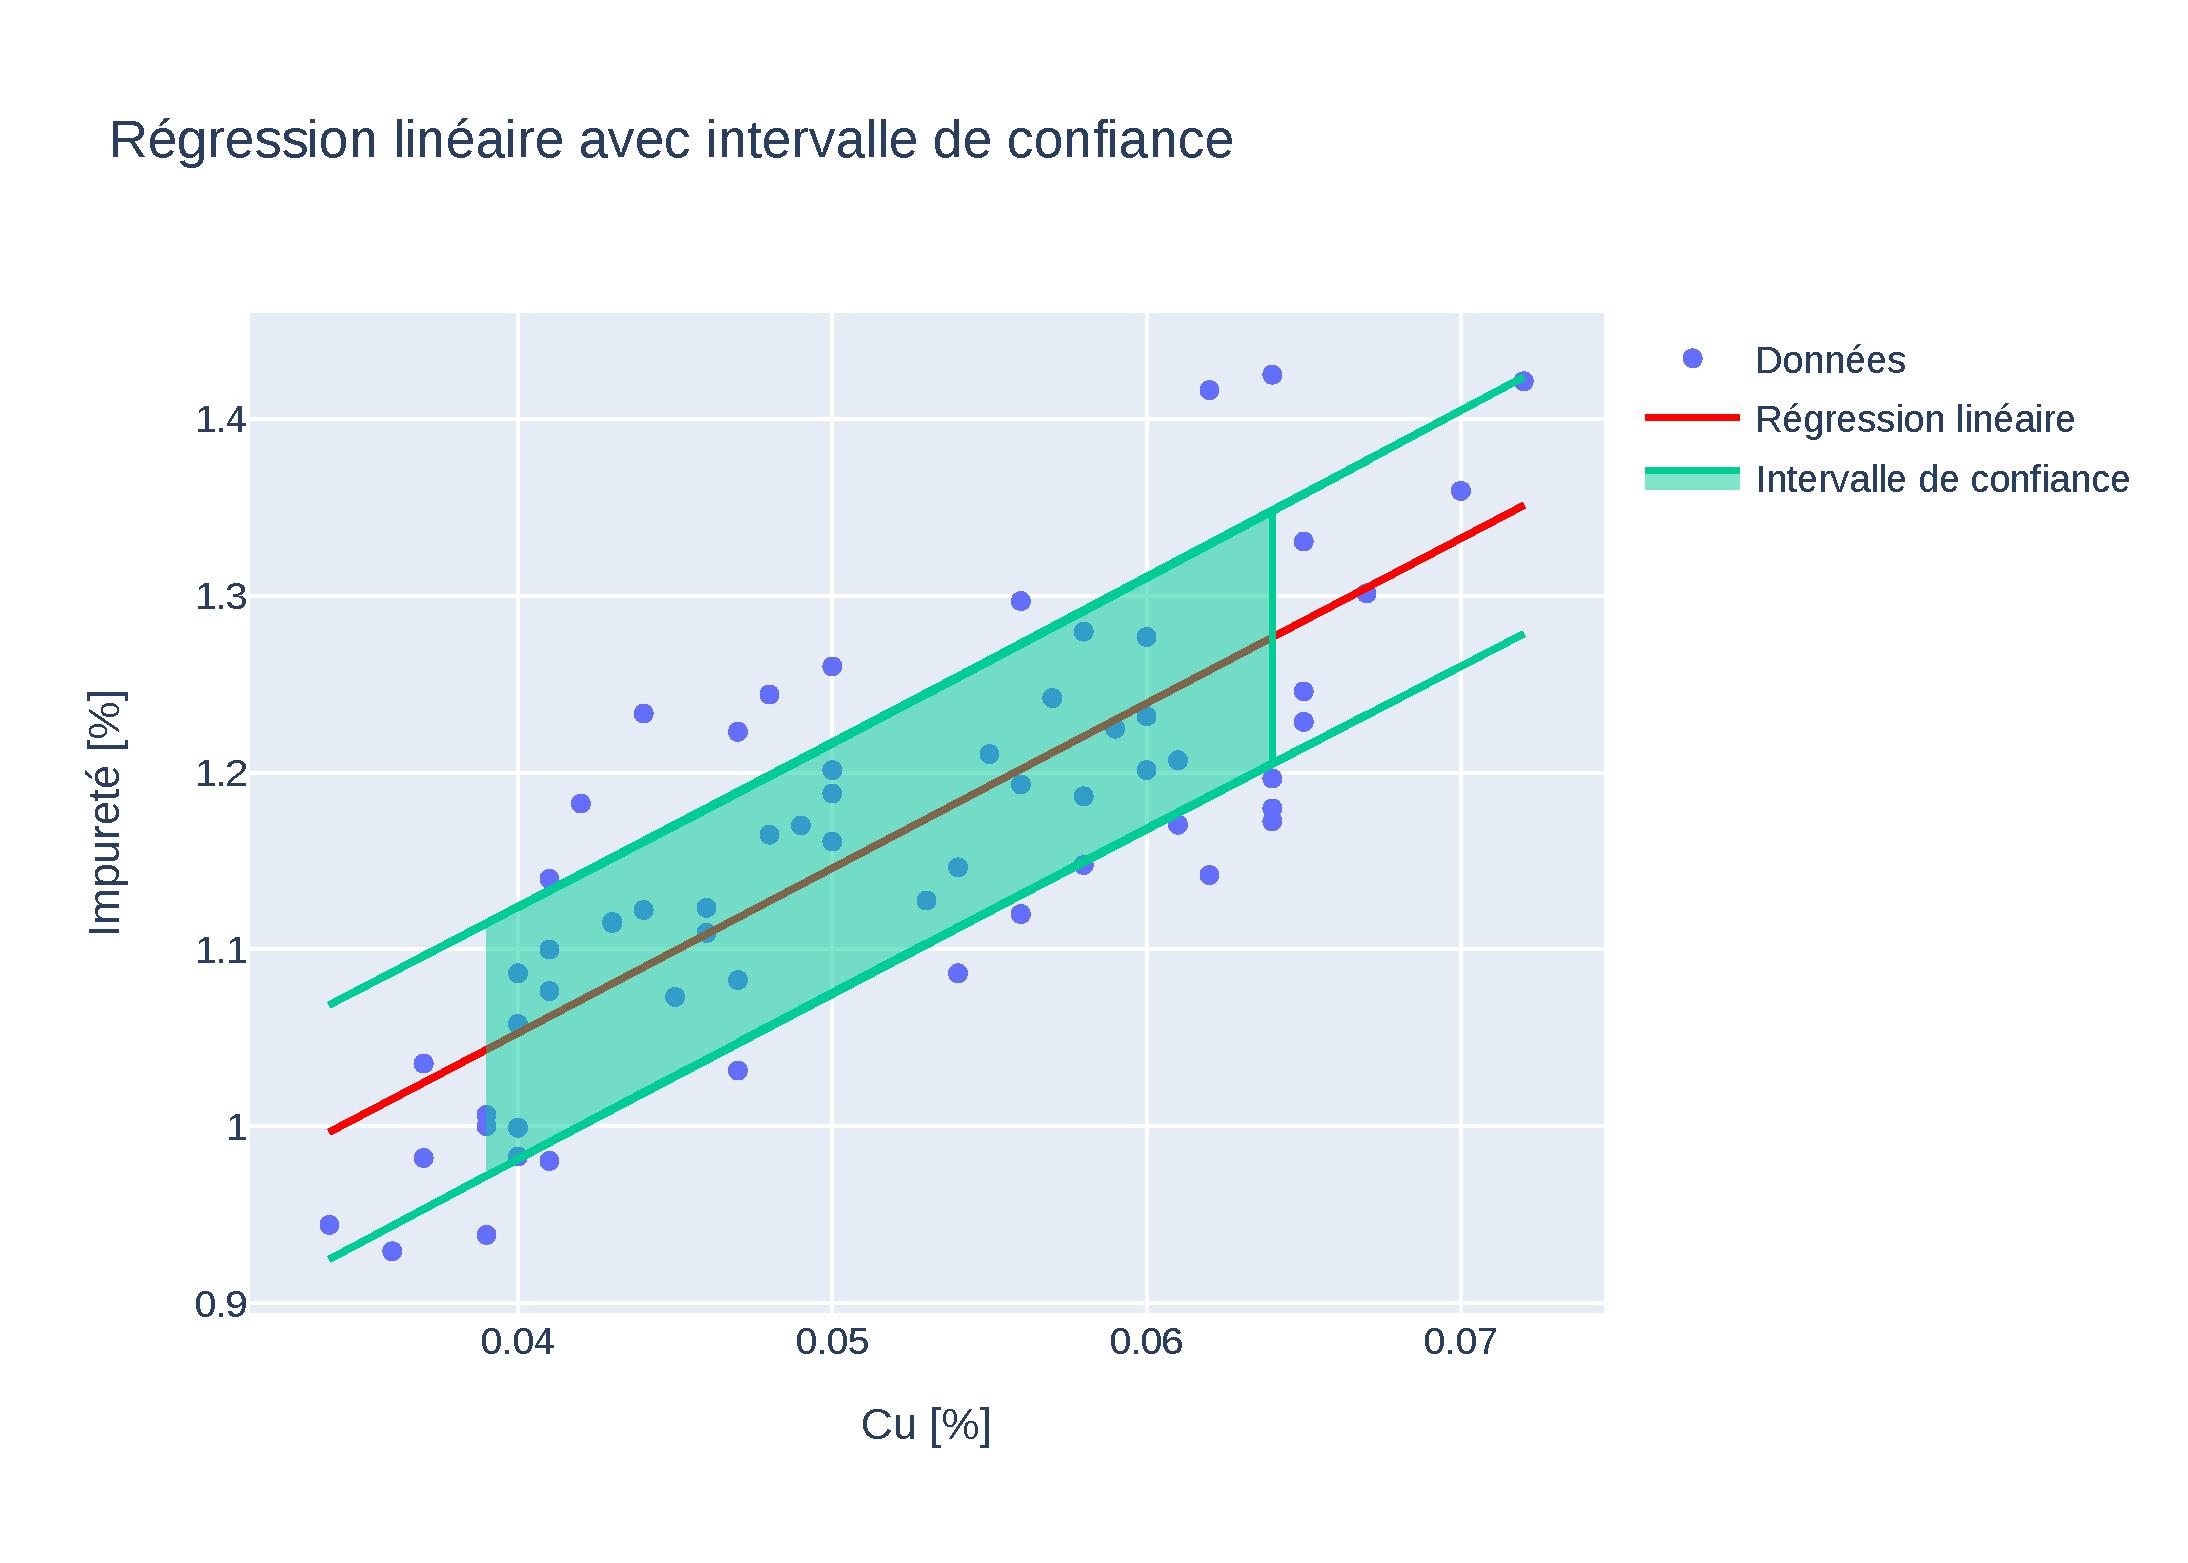
\includegraphics[scale=1]{Images/Statistique/Regression_Impurete_Cu.pdf}
%     \end{adjustbox}
%     \caption{L'impureté en fonction de Sn et de Cu}
%     \label{fig:regression-impurete}
% \end{figure}



% % Regression linéaire entre Impurete et Sn, Cu ;et Ono  et Cr, Cu 
\begin{figure}[H]
    \centering
    \adjustbox{width=1.25\textwidth, center}{  % Ajuster à la largeur de la page
        \begin{minipage}{0.8\textwidth}
            \centering
            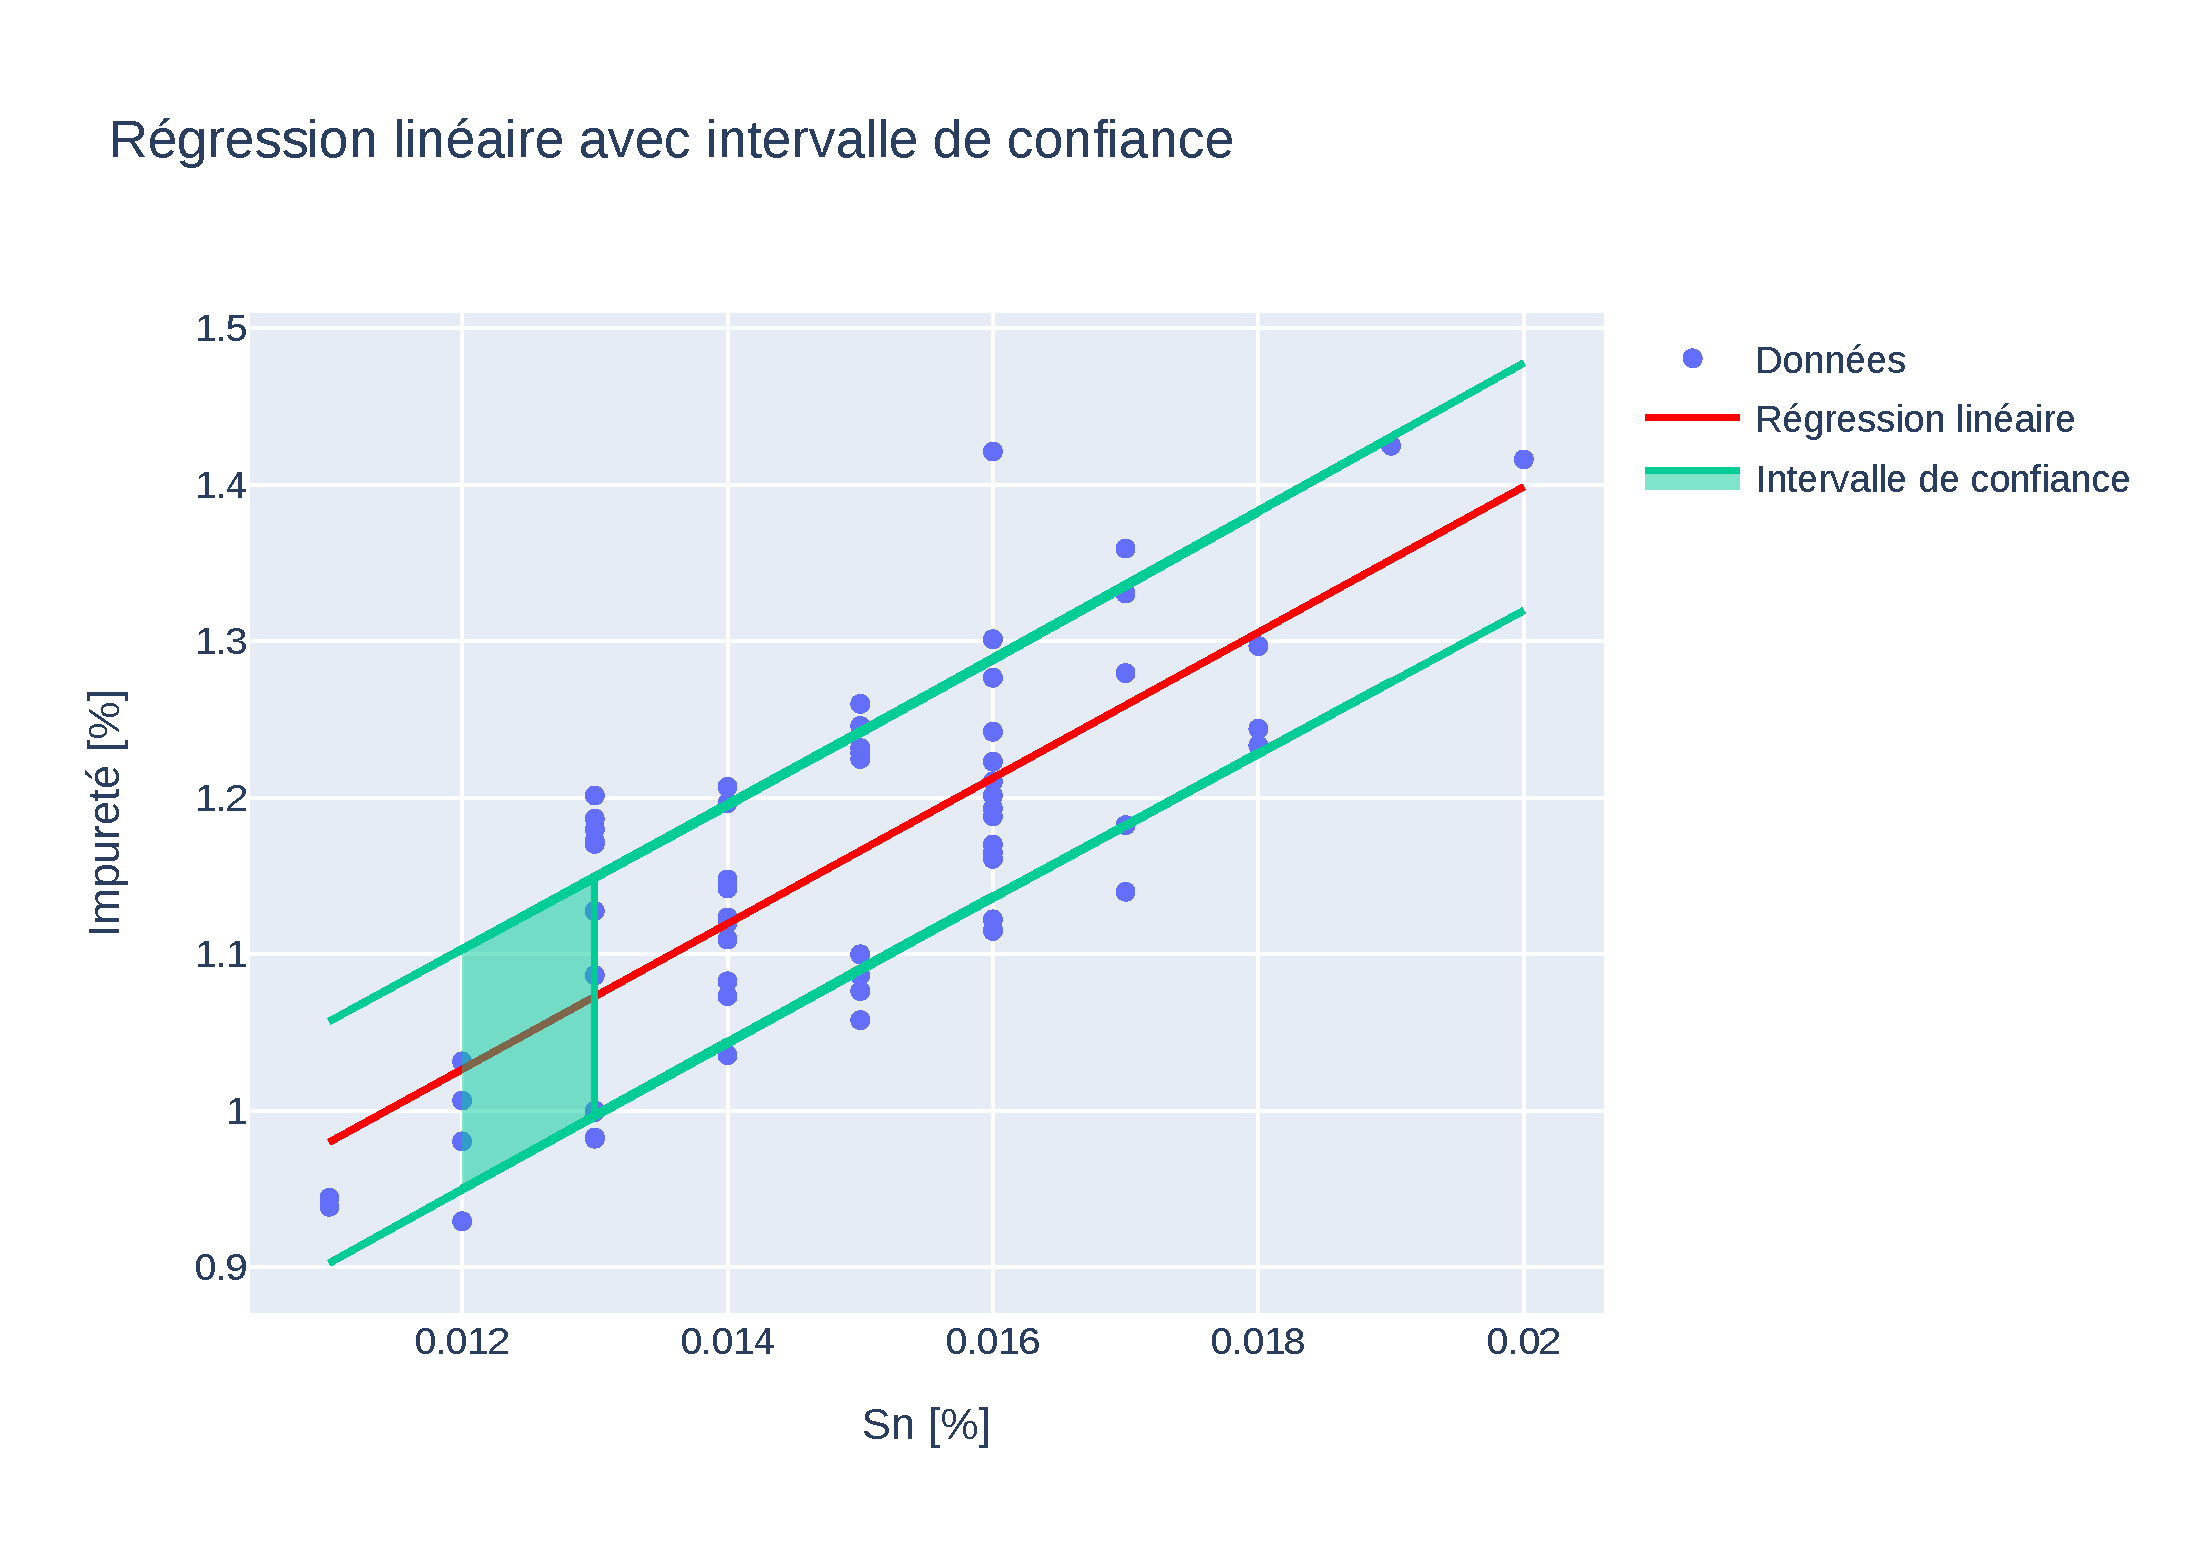
\includegraphics[width=\textwidth]{Images/Statistique/Regression_Impurete_Sn.pdf}
        \end{minipage}
        \hspace{0.01\textwidth}  % Petit espacement entre les colonnes
        \begin{minipage}{0.8\textwidth}
            \centering
            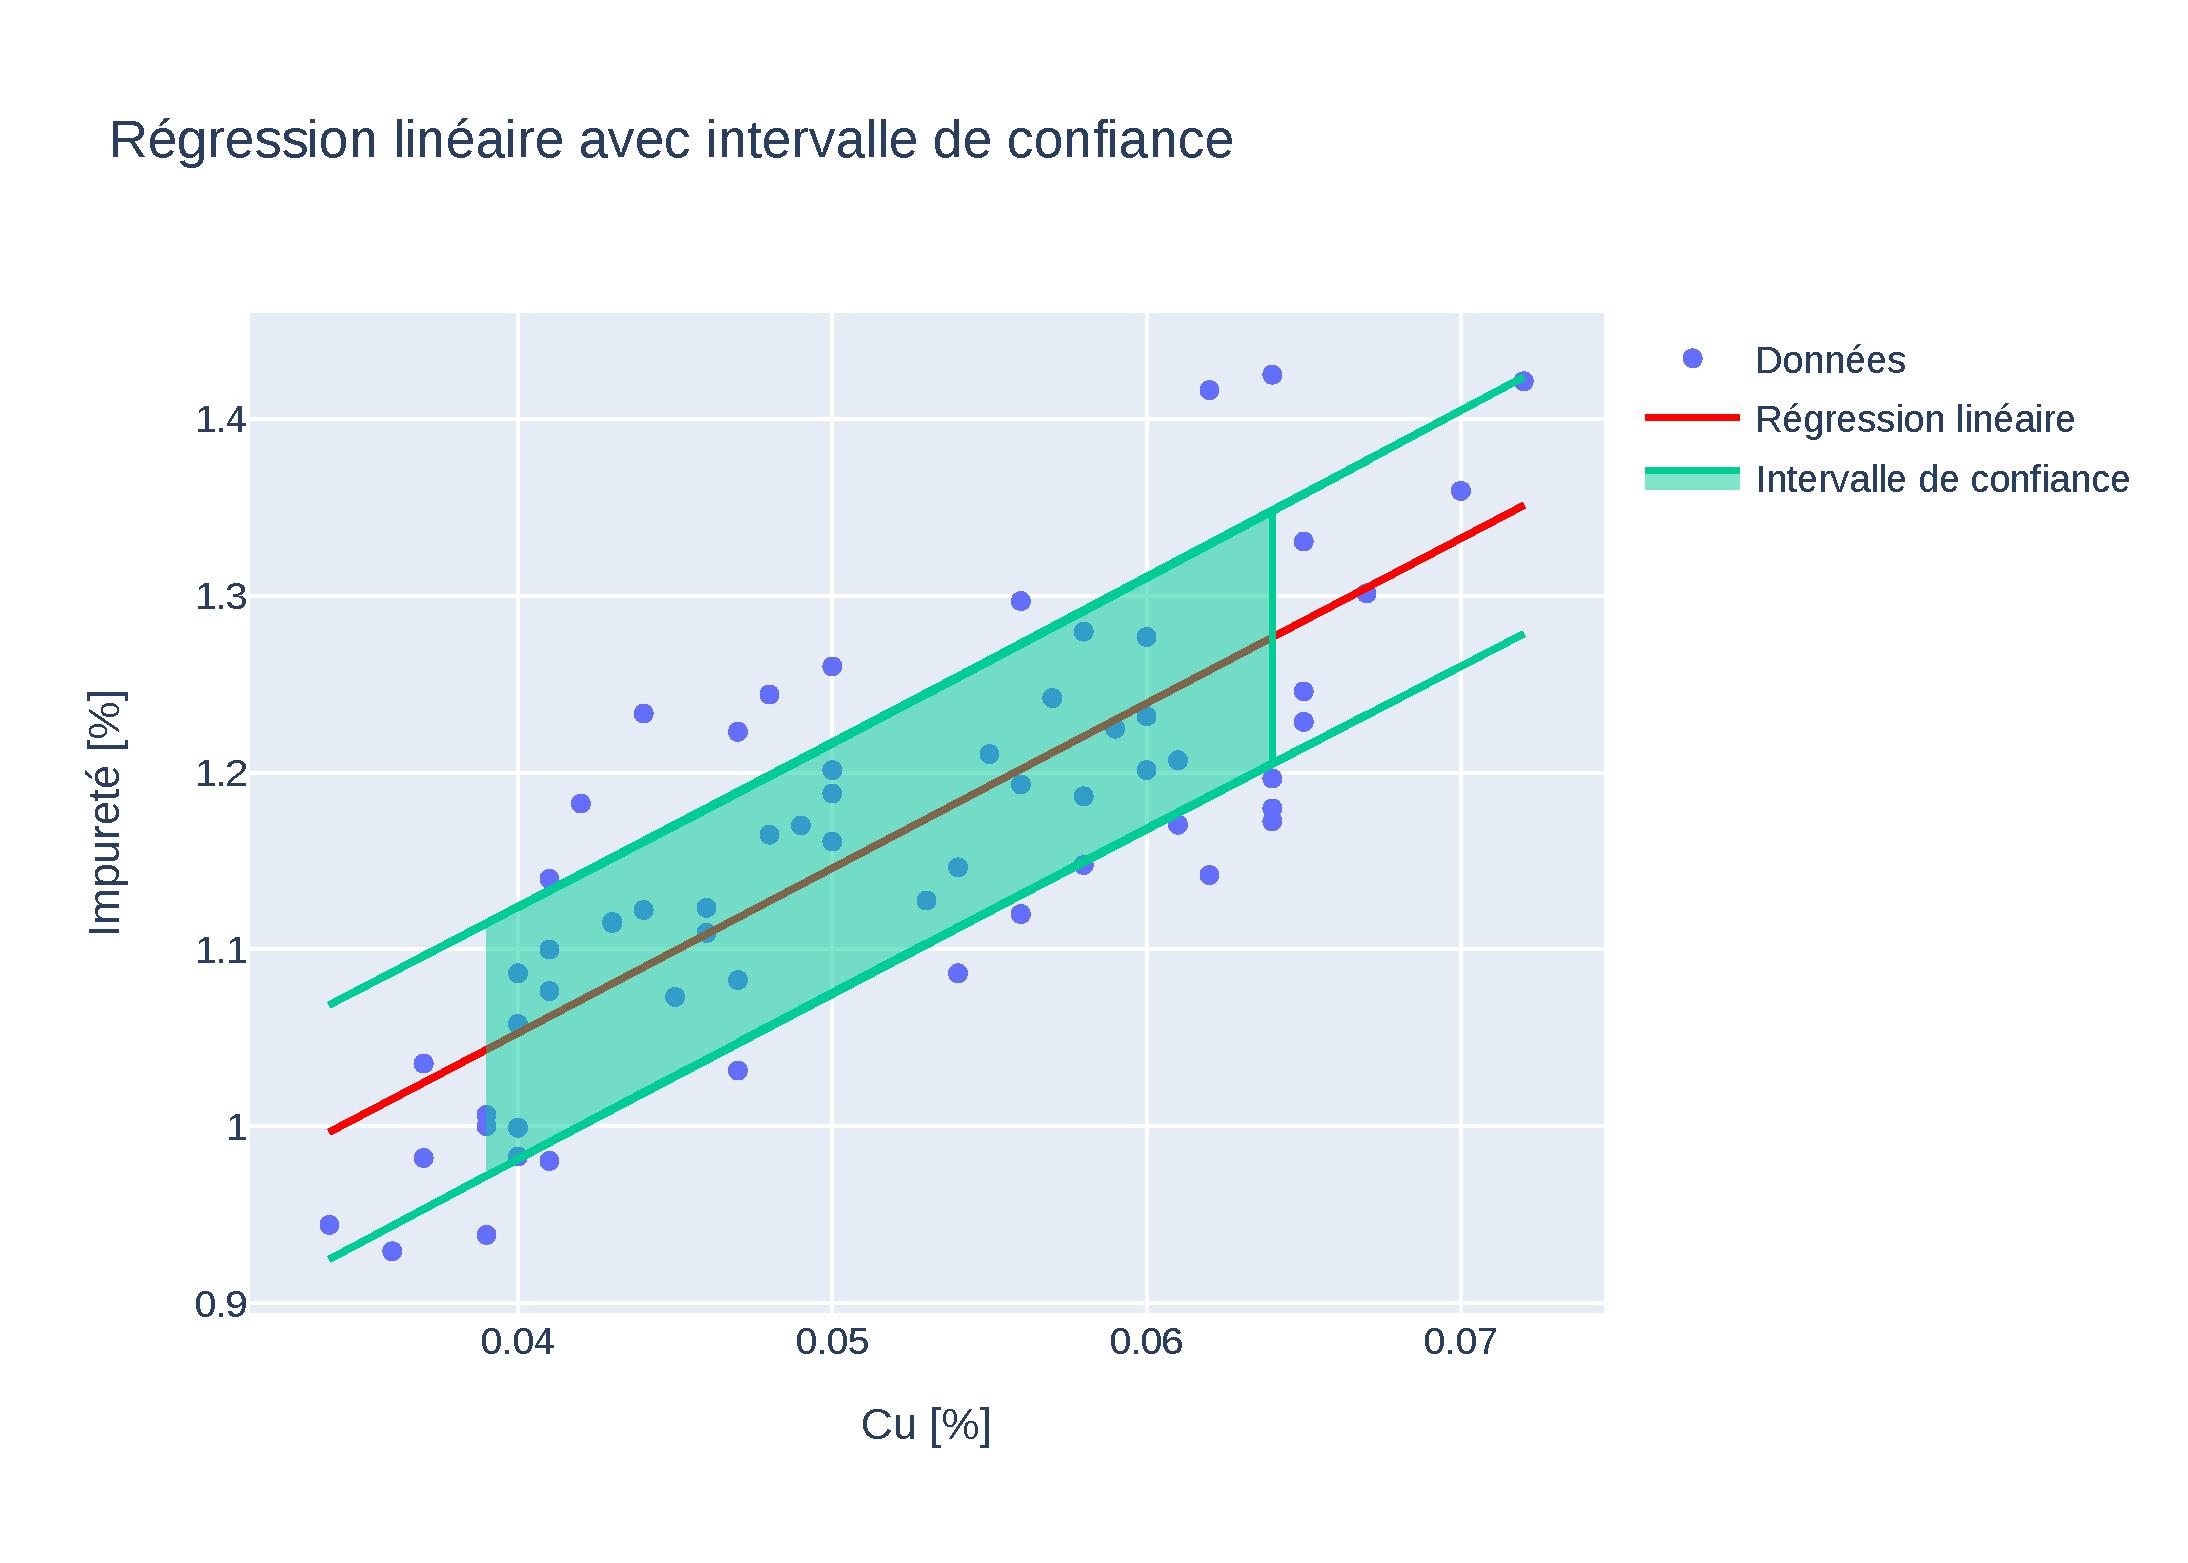
\includegraphics[width=\textwidth]{Images/Statistique/Regression_Impurete_Cu.pdf}
        \end{minipage}
    }\\[0.5cm]  % Espacement vertical entre les rangées
    \adjustbox{width=1.25\textwidth, center}{
        \begin{minipage}{0.8\textwidth}
            \centering
            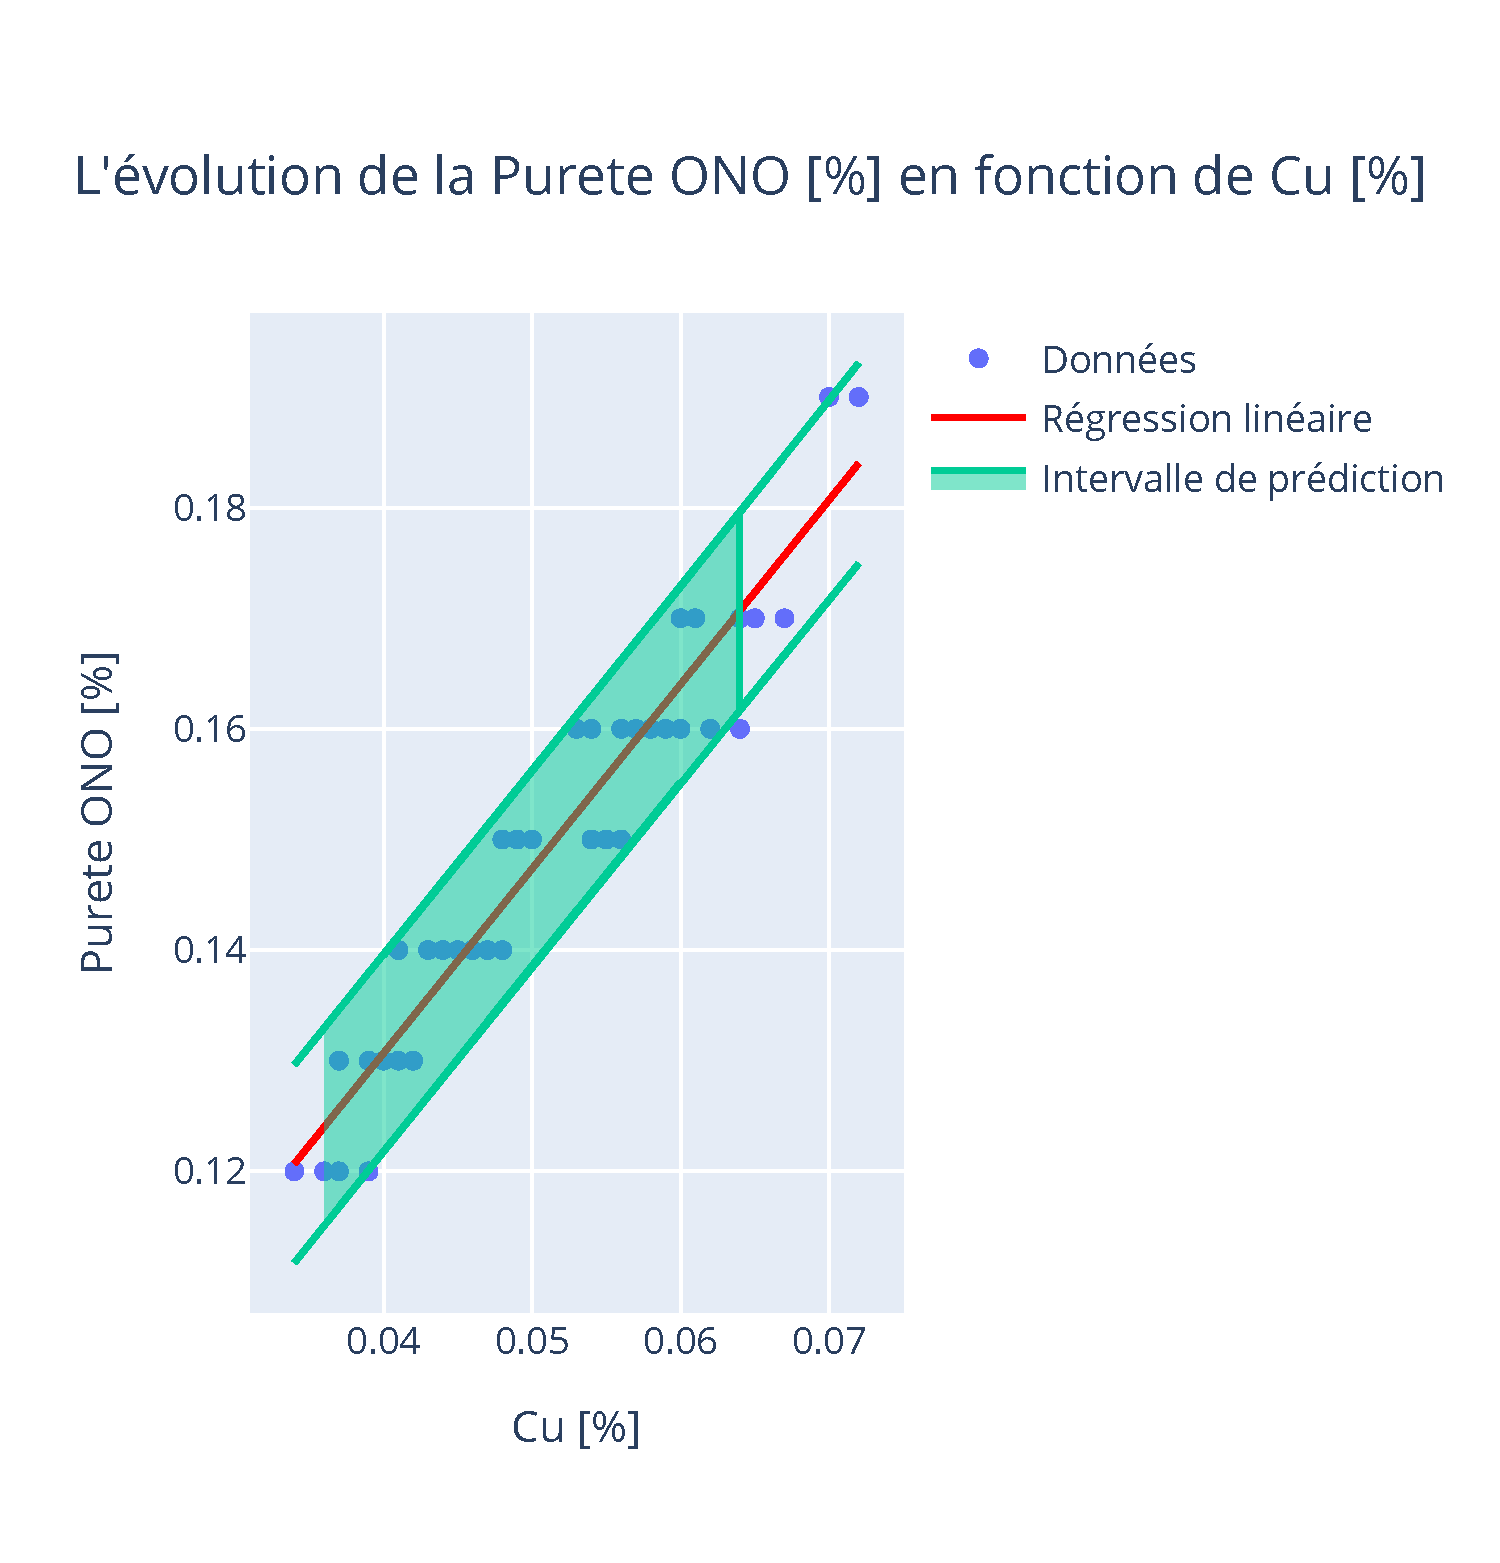
\includegraphics[width=\textwidth]{Images/Statistique/Regression_Ono_Cu.pdf}
        \end{minipage}
        \hspace{0.01\textwidth}  % Petit espacement entre les colonnes
        \begin{minipage}{0.8\textwidth}
            \centering
            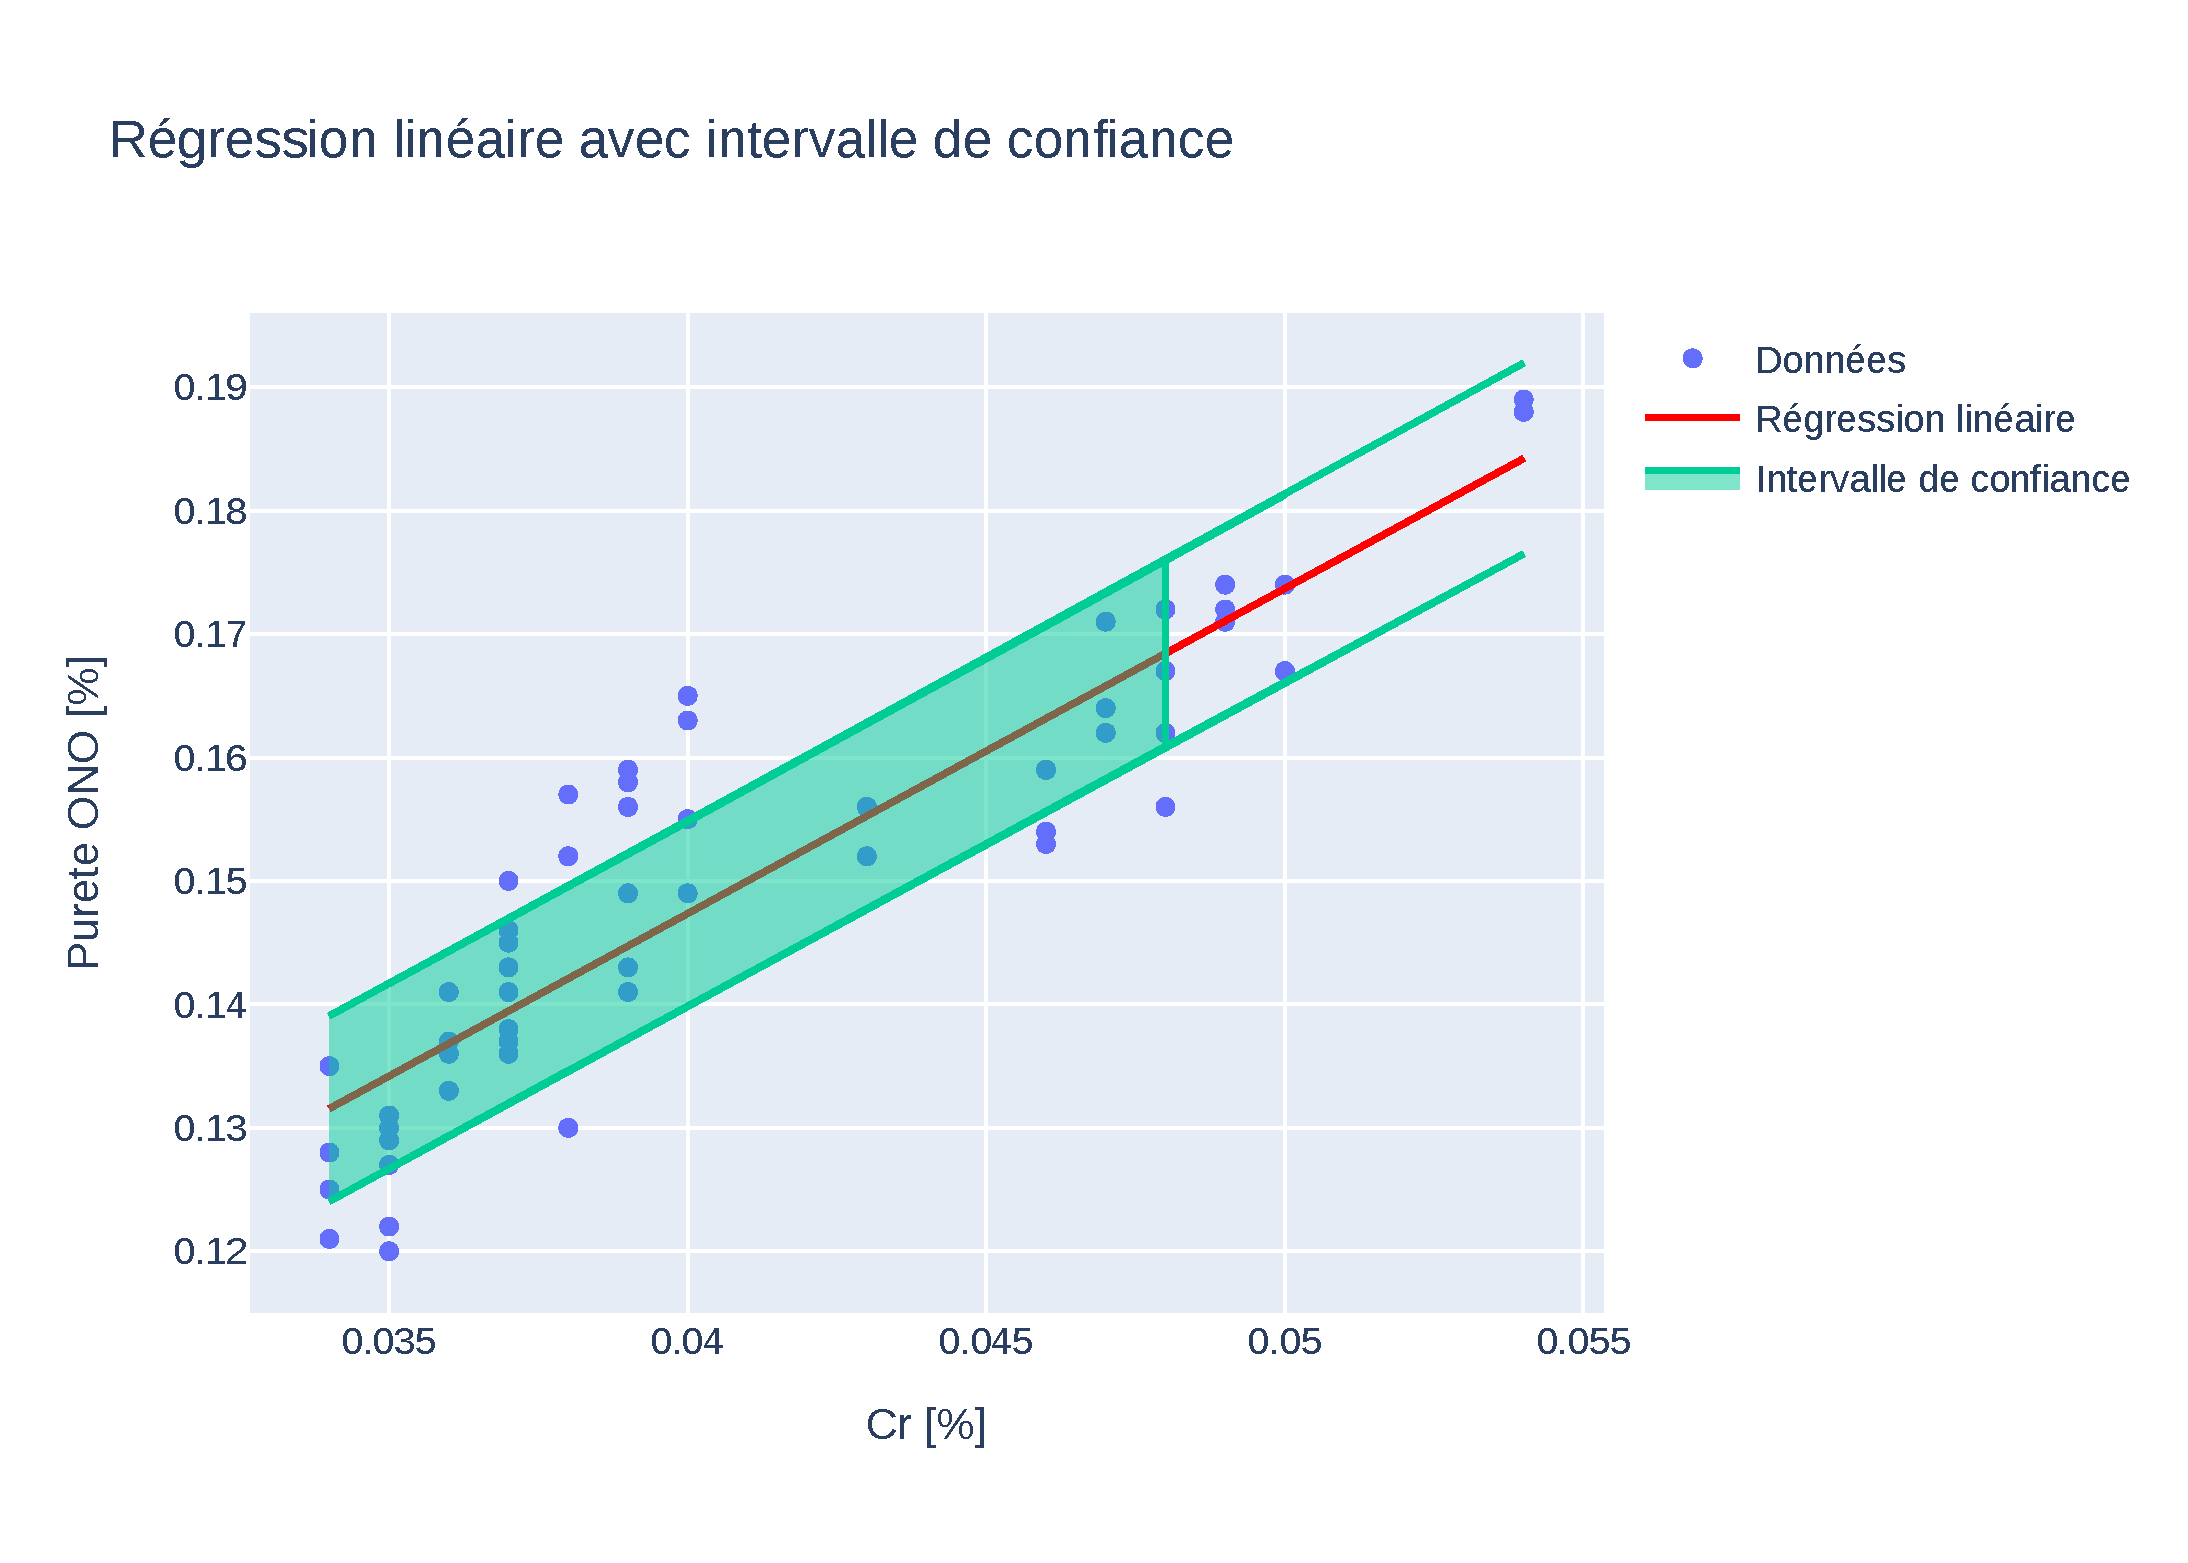
\includegraphics[width=\textwidth]{Images/Statistique/Regression_Ono_Cr.pdf}
        \end{minipage}
    }
    \caption{L'évolution de la pureté Ono et l'impureté}
    % \caption{La régression linéaire et l'intervalle de prédiction de la pureté Ono en fonction de Cr et de Cu}
    \label{fig:regression}
\end{figure}














% % Rm

% \textbf{La Résistance mécanique en fonction du Cuivre} 
% \begin{figure}[H]
% 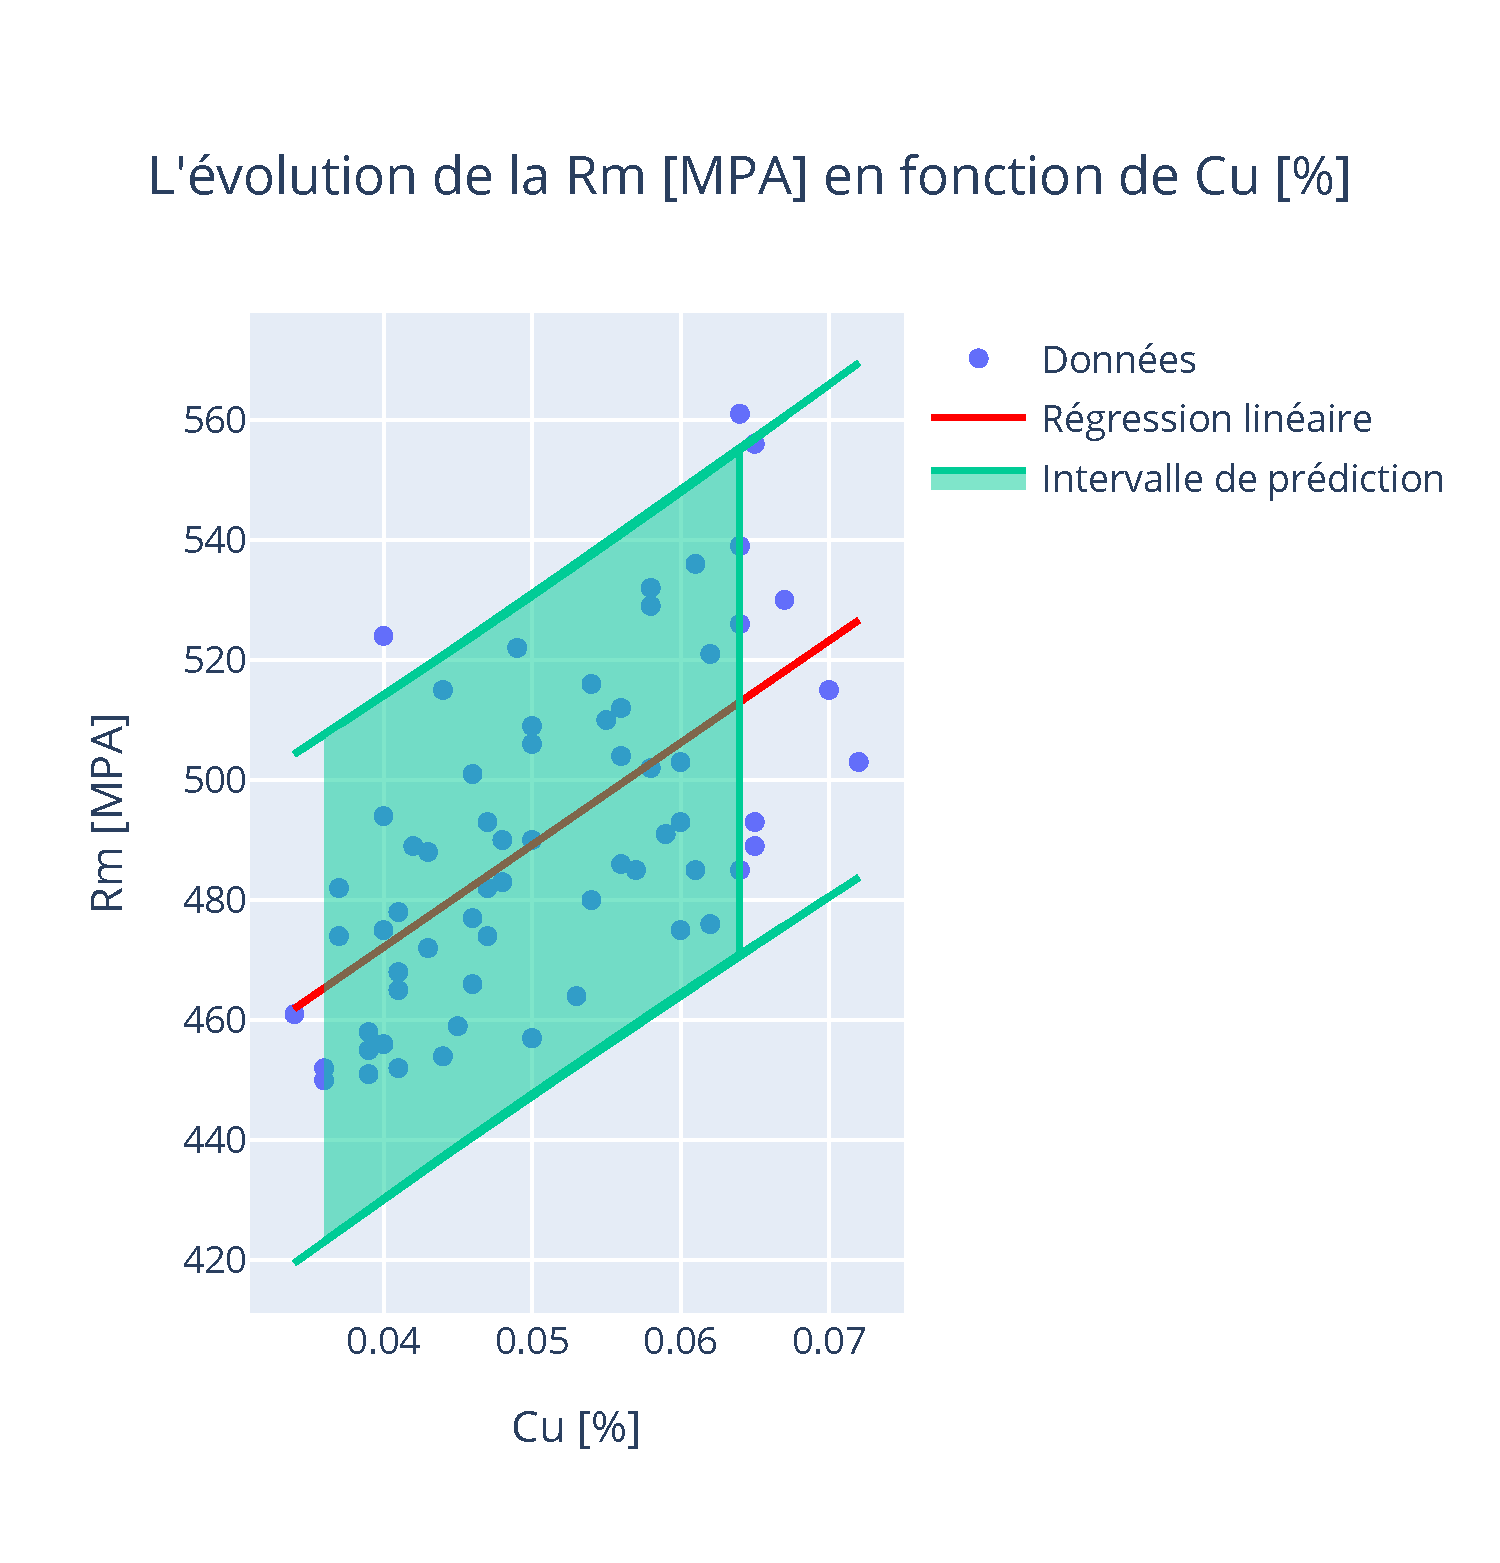
\includegraphics[width=\textwidth]{Images/Statistique/Regression_Cu_Rm.pdf} 
% \end{figure}

% \textbf{La Résistance mécanique en fonction du Sn} 
% \begin{figure}[H]
% 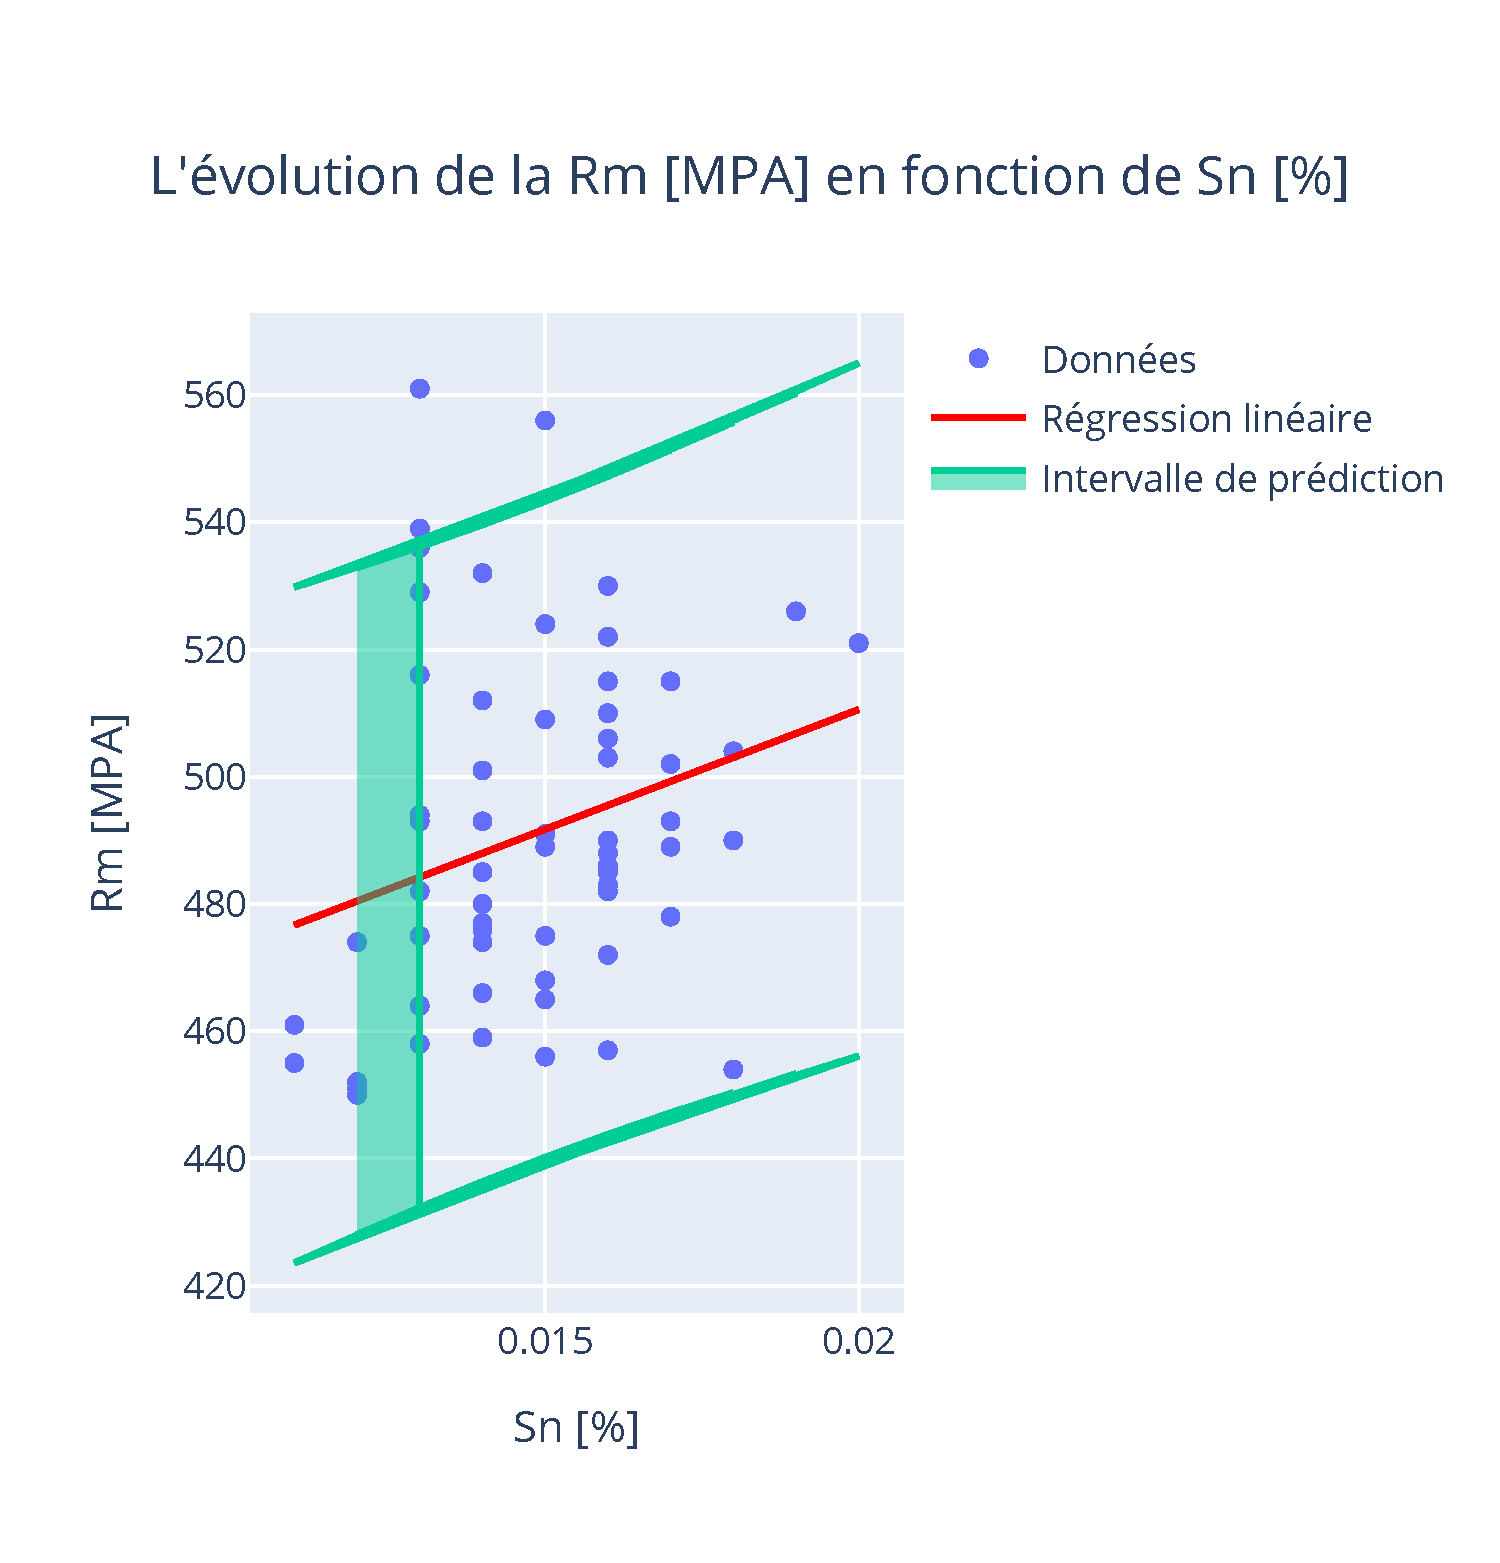
\includegraphics[width=\textwidth]{Images/Statistique/Regression_Sn_Rm.pdf} 
% \end{figure}


% % Allongement et Rm

% \textbf{La Résistance mécanique en fonction du Cr} 
% \begin{figure}[H]
% 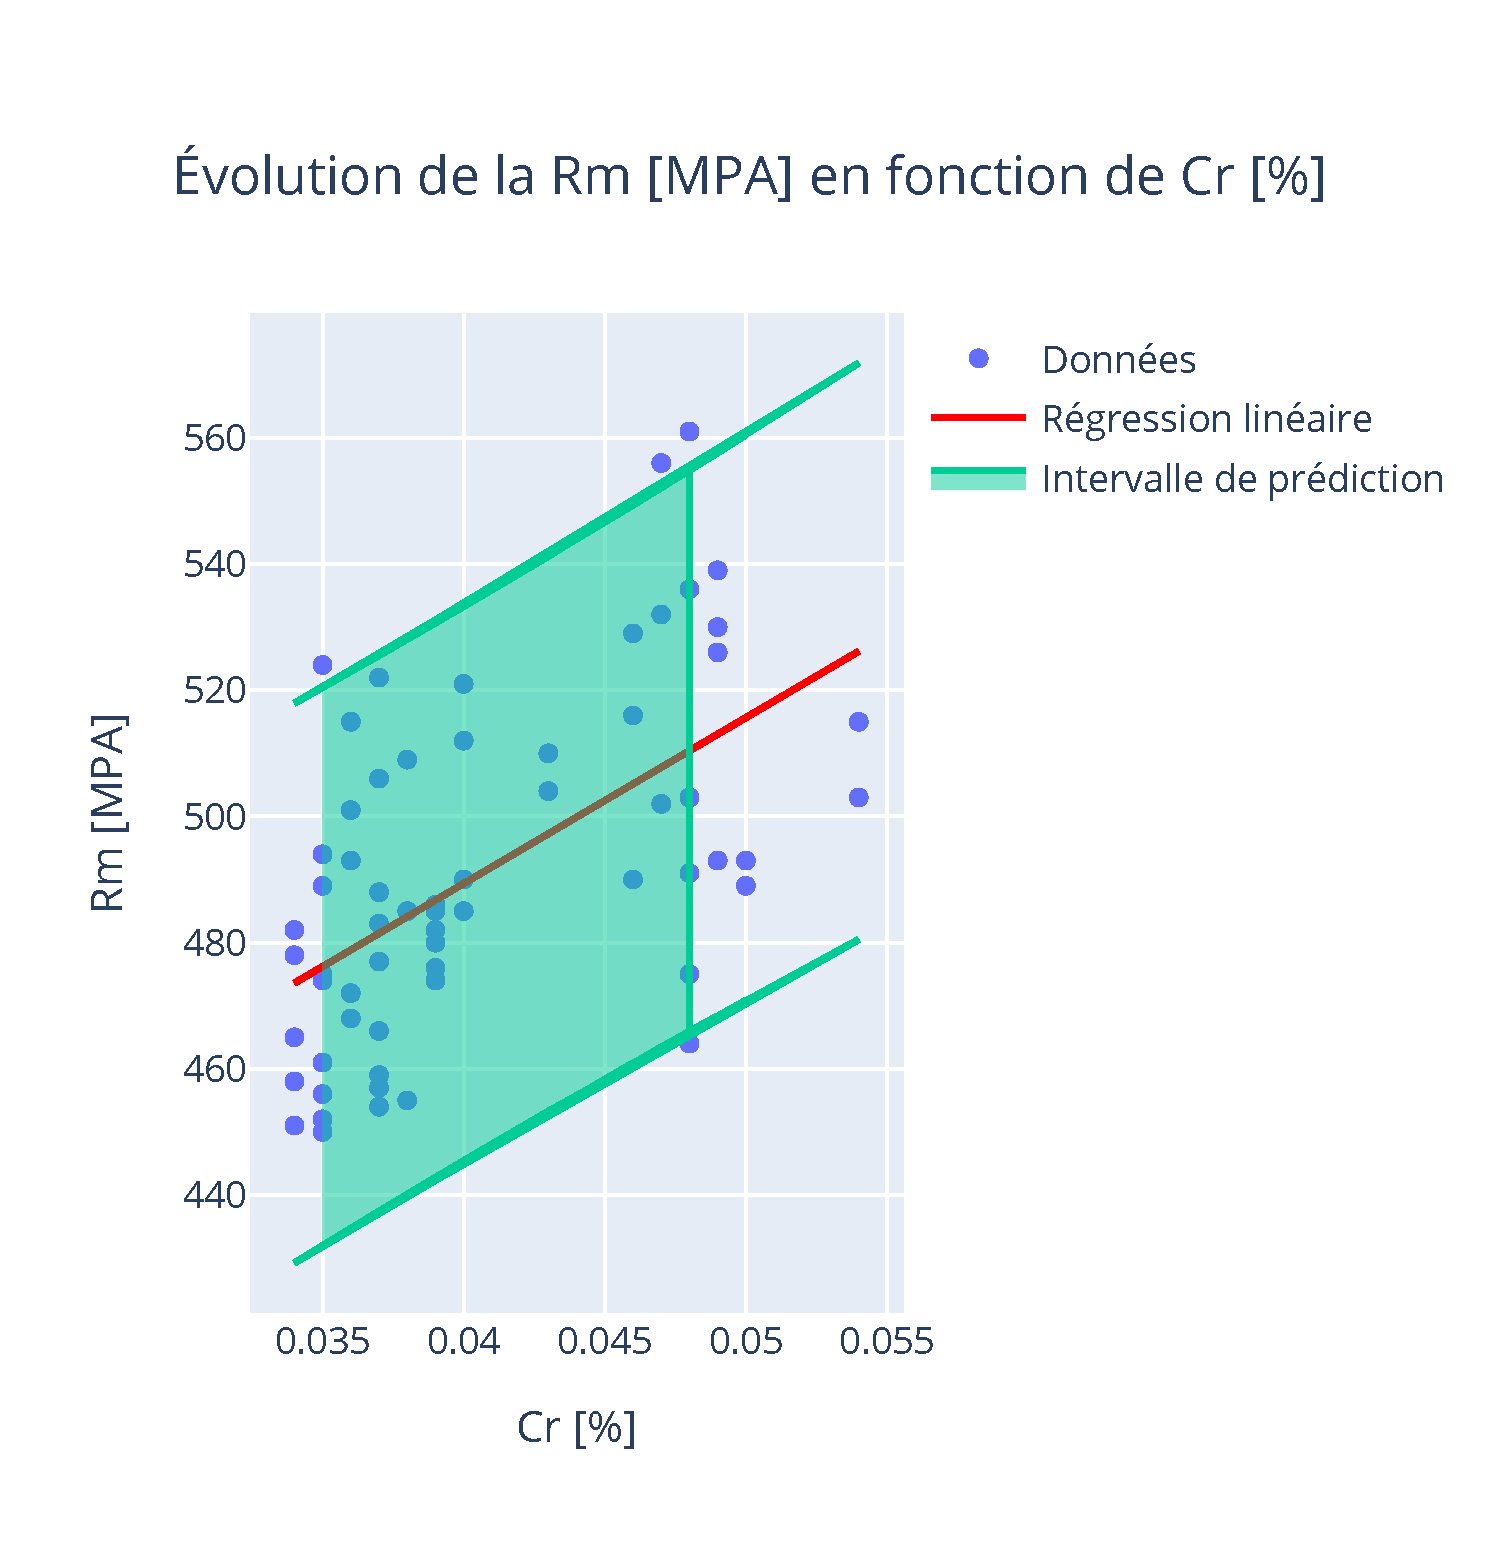
\includegraphics[width=\textwidth]{Images/Statistique/Regression_Cr_Rm.pdf} 
% \end{figure}


% \textbf{L'allongement en fonction du  Cr} 
% \begin{figure}[H]
% 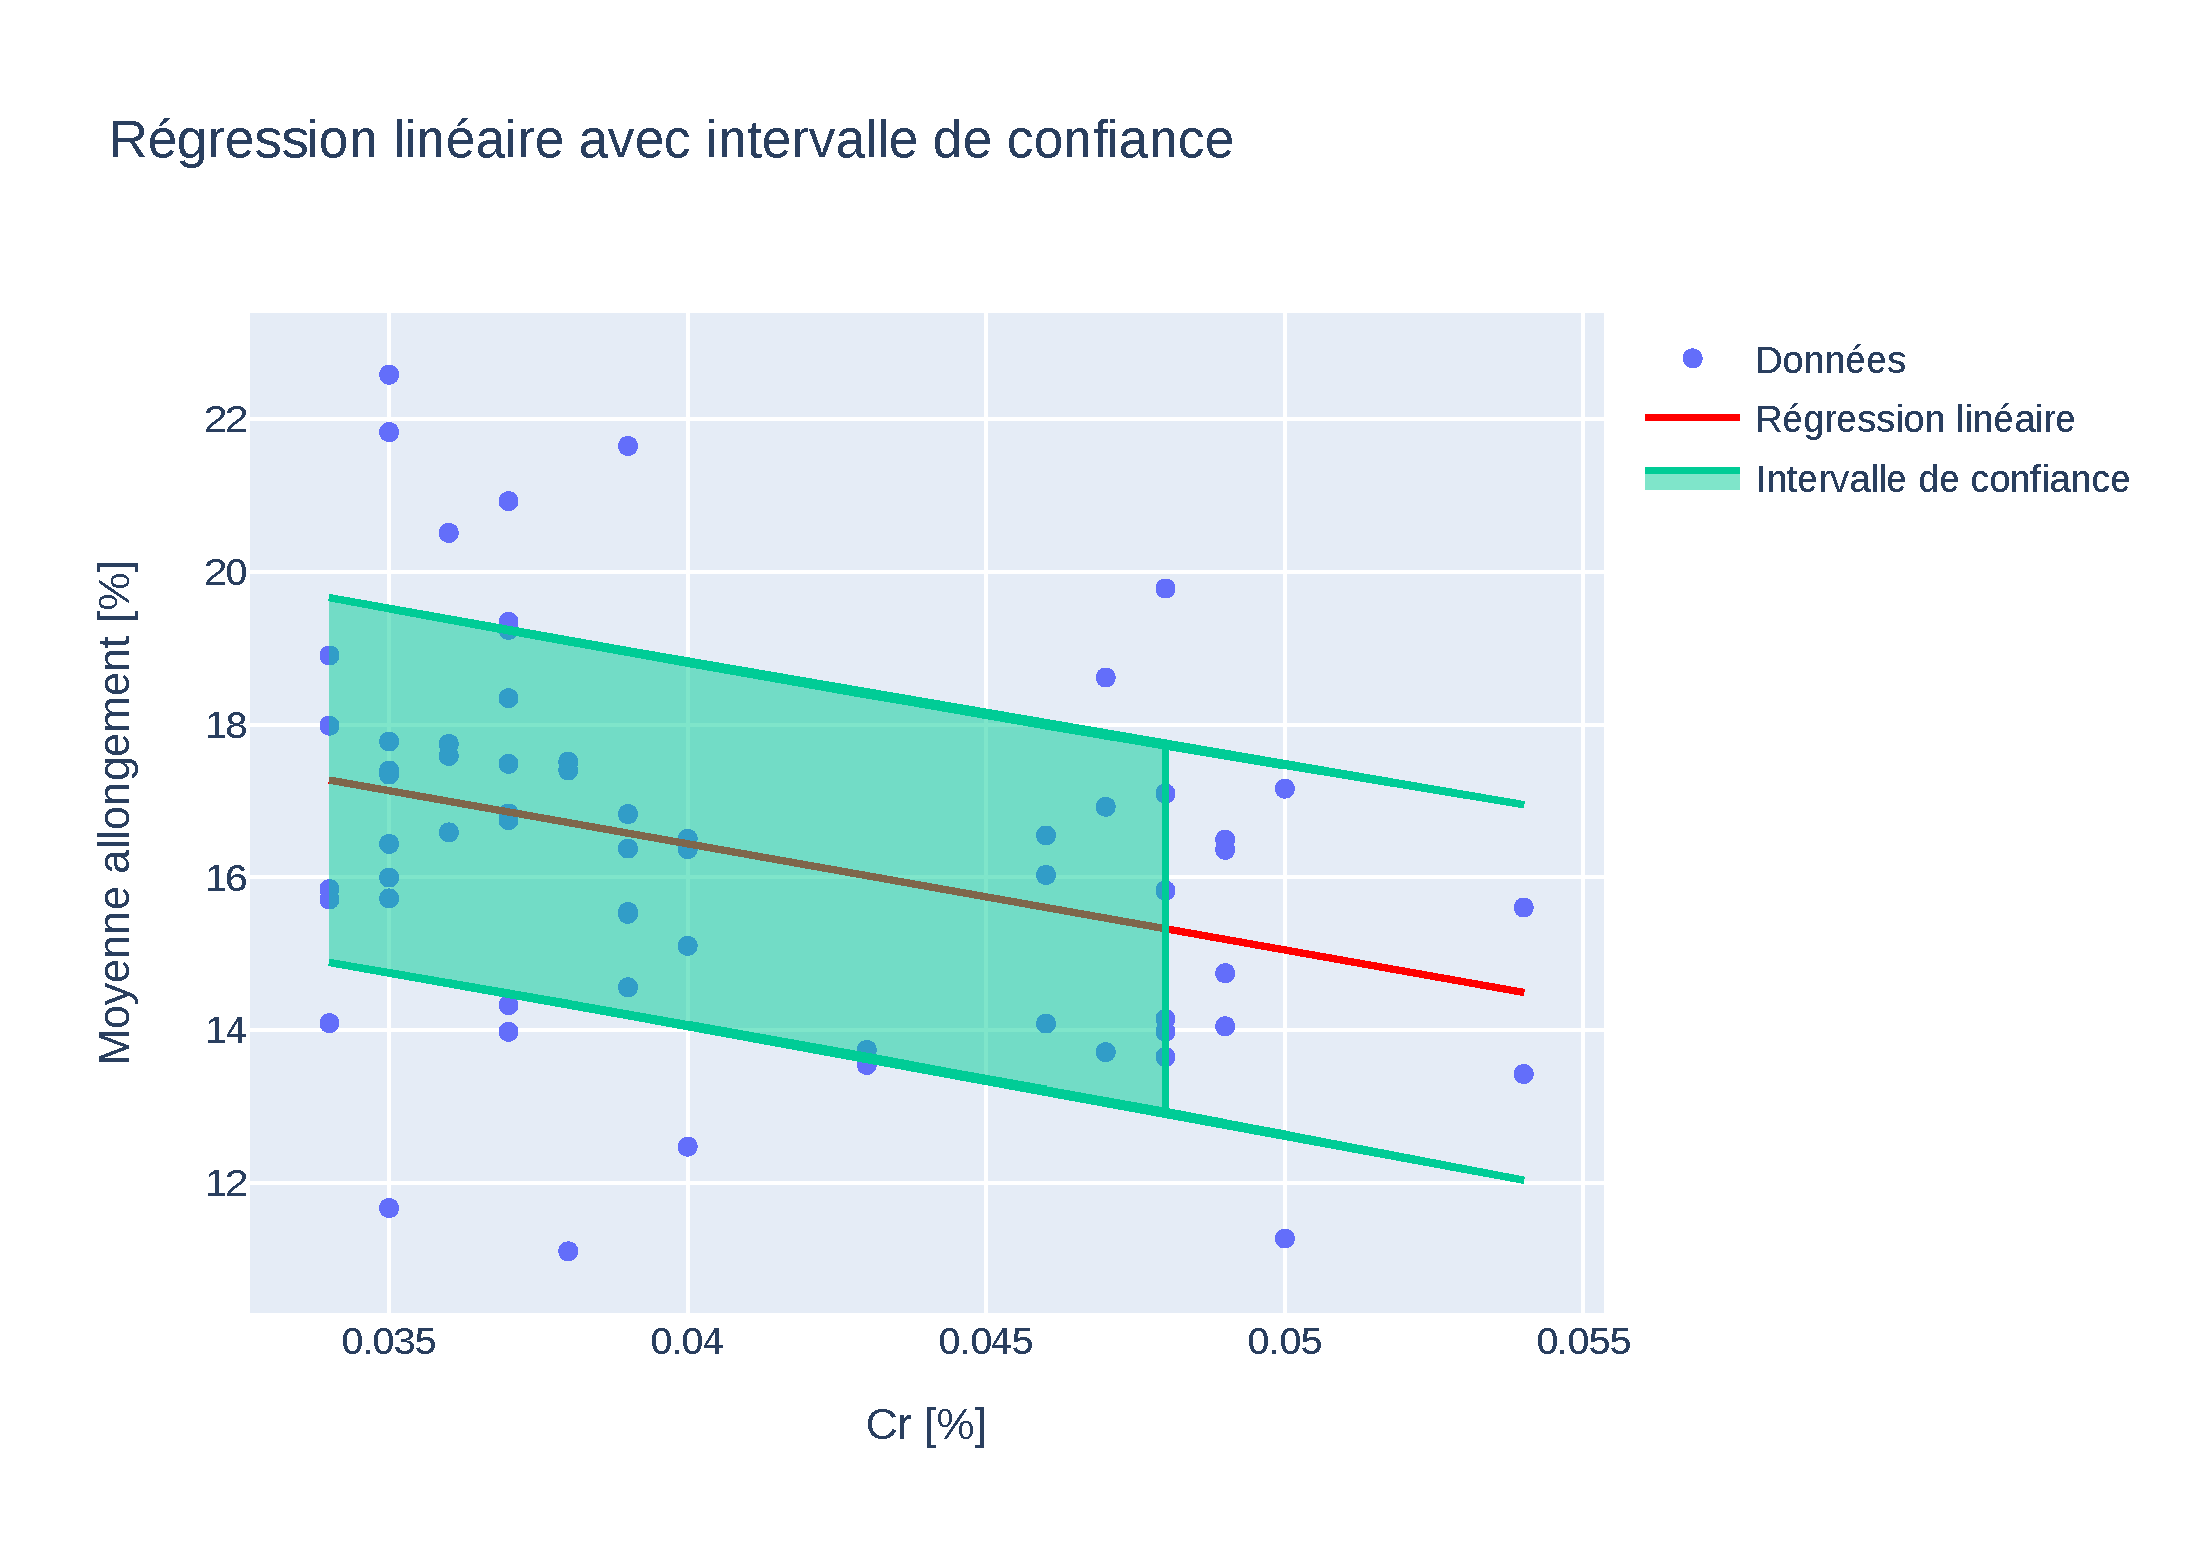
\includegraphics[width=\textwidth]{Images/Statistique/Regression_Cr_Allongement.pdf} 
% \end{figure}



% % Allongement

% \textbf{L'allongement en fonction du Cuivre} 
% \begin{figure}[H]
% 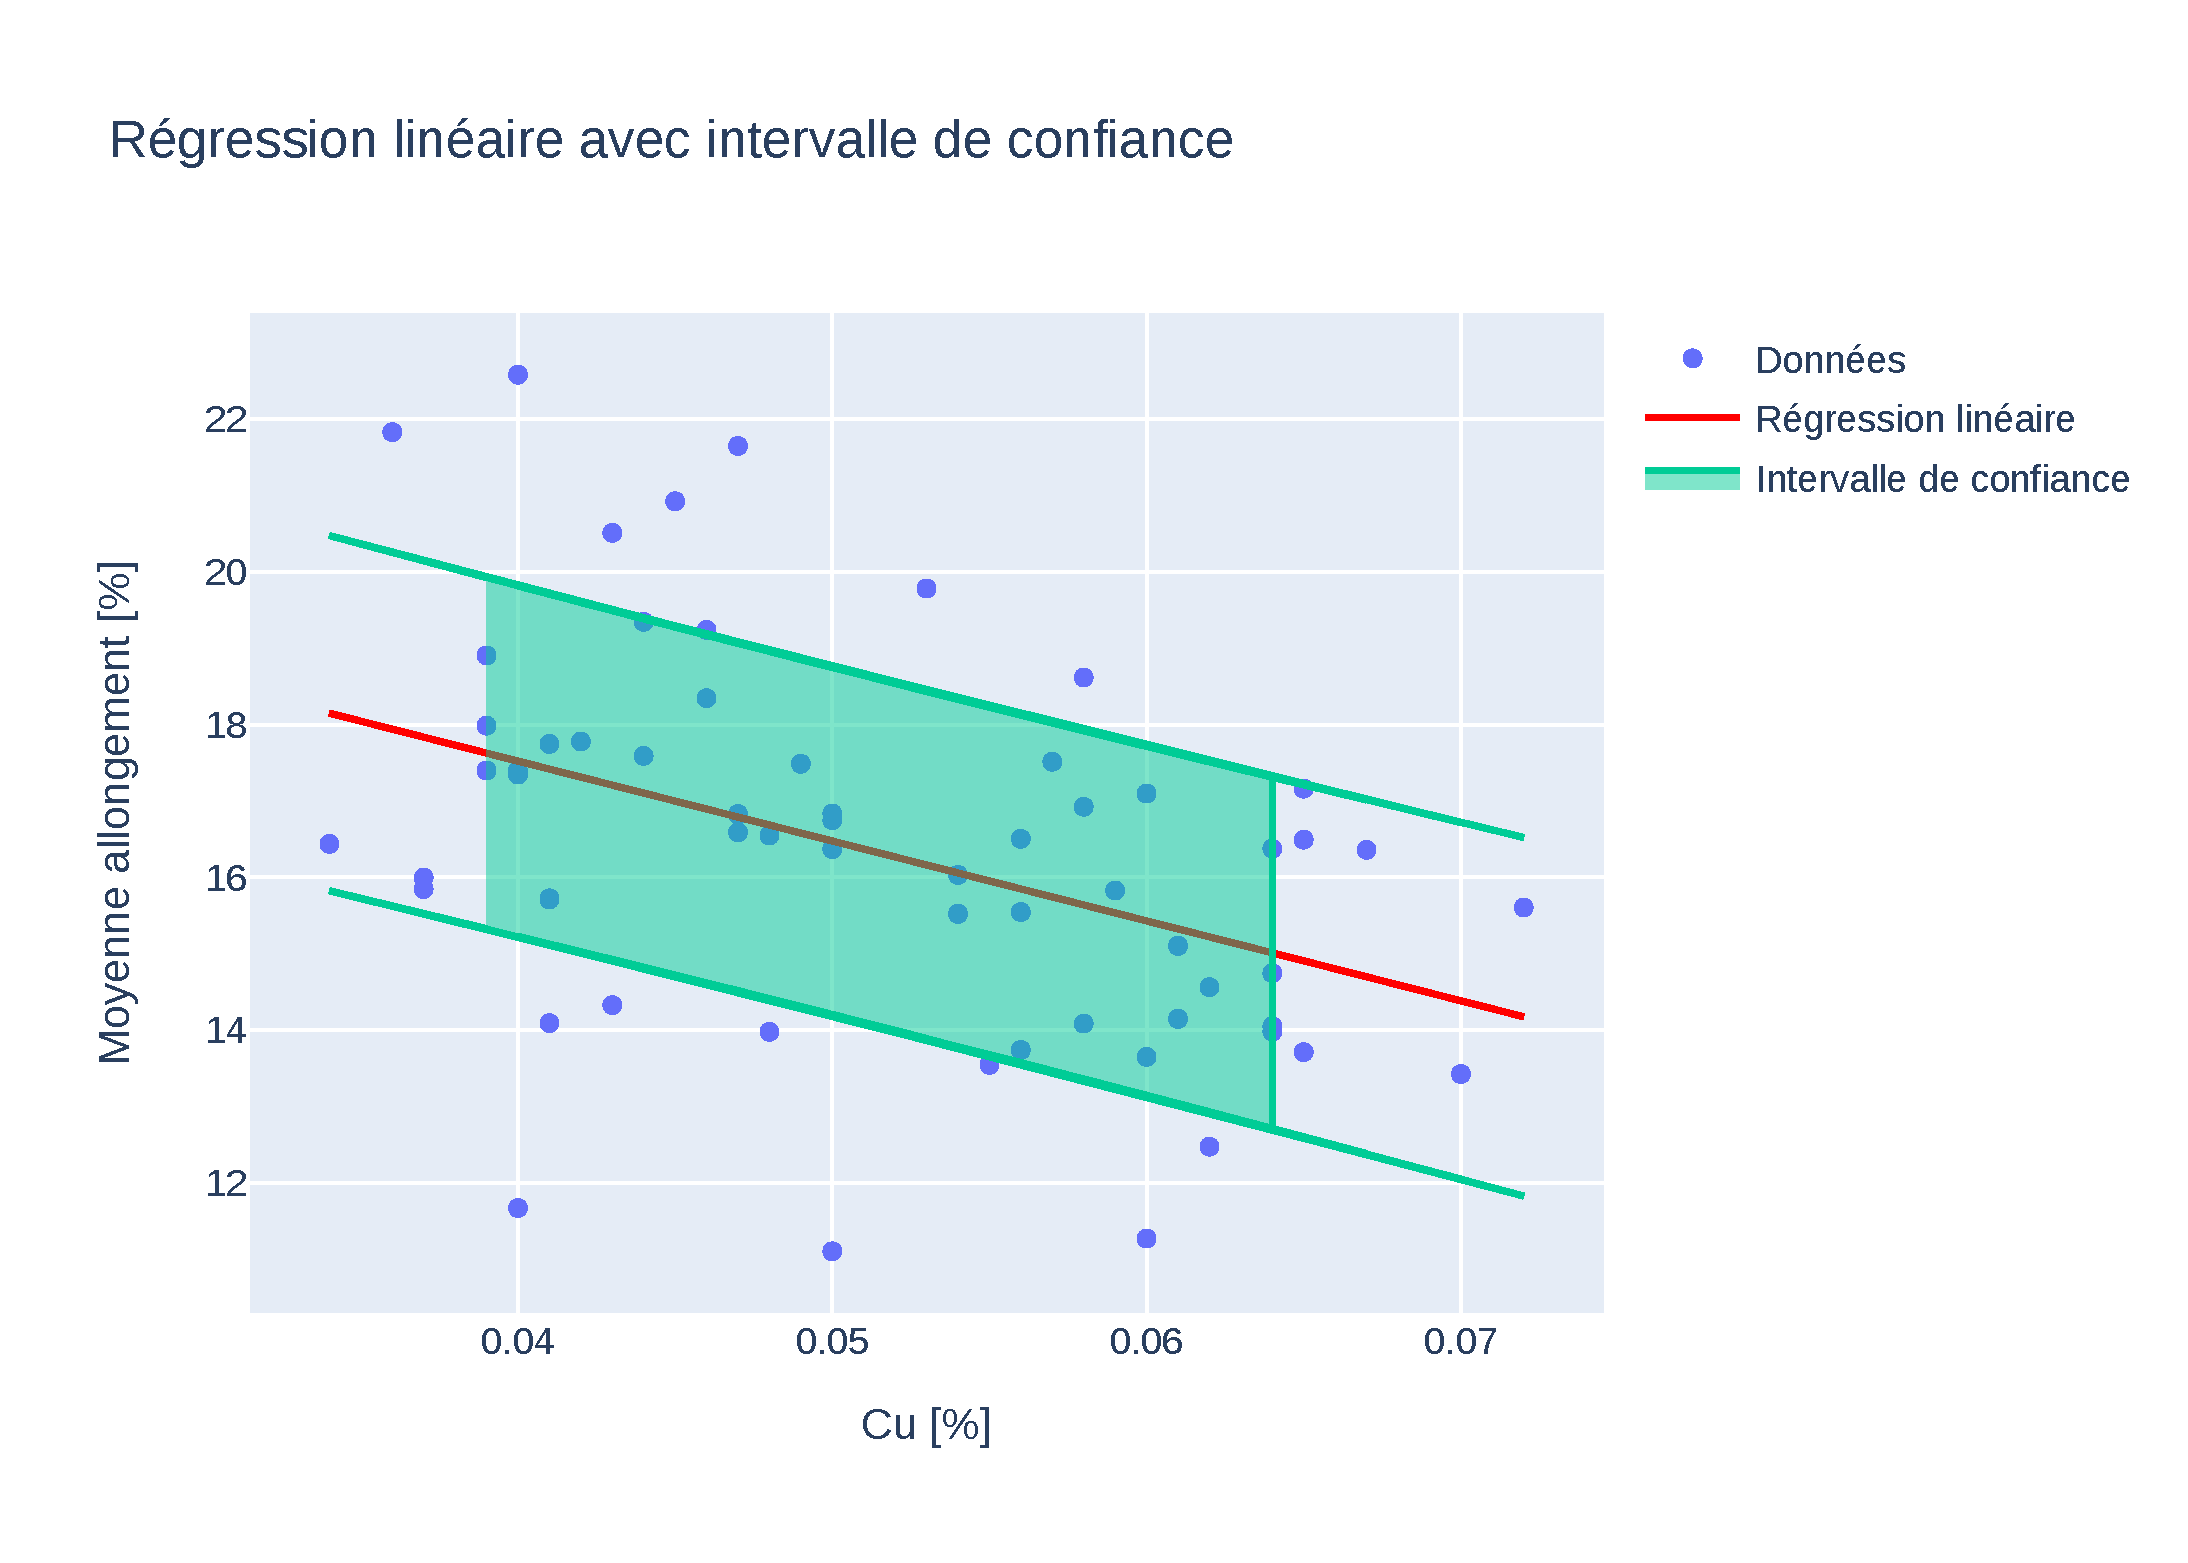
\includegraphics[width=\textwidth]{Images/Statistique/Regression_Cu_Allongement.pdf} 
% \end{figure}


% \textbf{L'allongement en fonction du Sn}
% \begin{figure}[H]
% 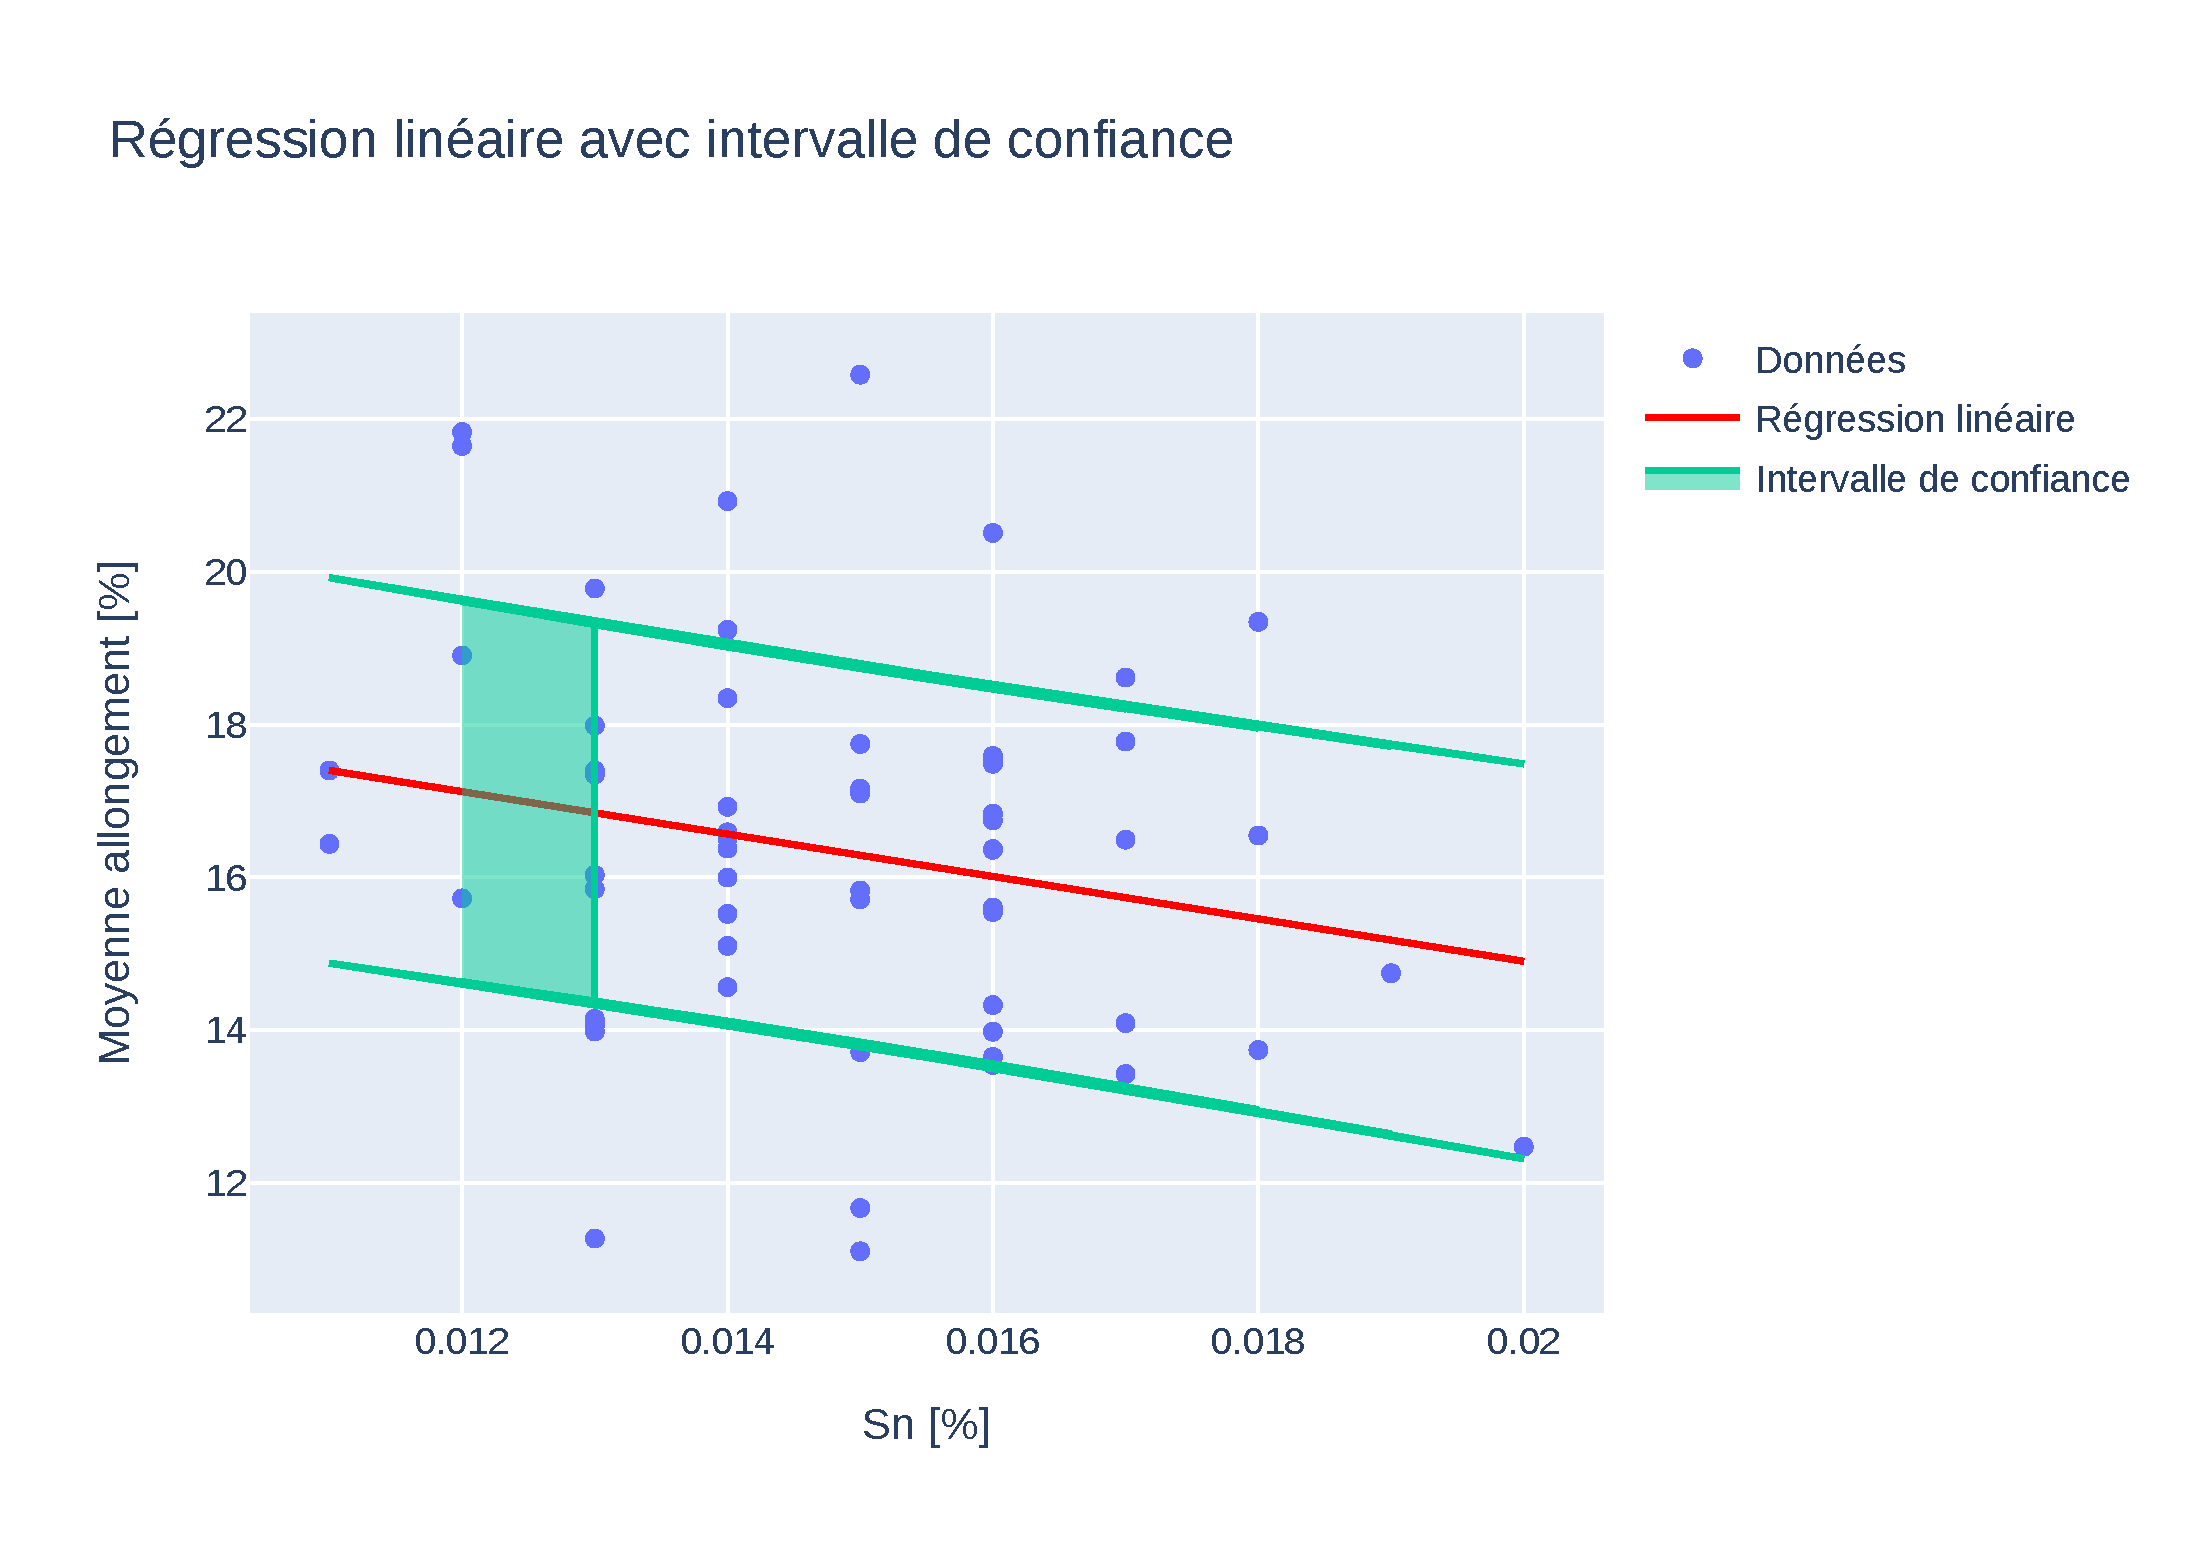
\includegraphics[width=\textwidth]{Images/Statistique/Regression_Sn_Allongement.pdf} 
% \end{figure}





\subsection{Conclusion}


% Conclusion 

Nous constatons une corrélation linéaire entre le cuivre et la résistance mécanique, ainsi qu'entre le cuivre et l'allongement. En revanche, pour les autres éléments, la linéarité n'est pas  évidente.



\textbf{Intervalles de confiance des indicateurs :}
\begin{itemize}
\item Impureté : [1.13, 1.19]
\item Pureté ONO : [0.145, 0.153]
\end{itemize}

\textbf{Intervalles de confiance des éléments chimiques :}
\begin{itemize}
\item Sn (Étain) : [0.0143, 0.0153]
\item Cu (Cuivre) : [0.0488, 0.0538]
\item Cr (Chrome) : [0.0392, 0.0422]
\item V (Vanadium) : [0.00092, 0.00111]
\end{itemize}


















\section{La recette Optimale}

\subsection{Présentation du problème de la Recette }

Dans le cadre du processus de fabrication de 5 tonnes de fontes, l'une des étapes préliminaires fondamentales
réside dans la détermination du lit de fusion, c'est-à-dire la proportion des matières premières
nécessaires à la fusion. Dans notre cas, on souhaite  produire 5 tonne de fonte de haute qualité.
Pour ce faire, nous disposons d'une trentaine de matières premières, chacune possédant sa propre
composition chimique distinctive. Chaque matière première est disponible ou non en quantité limitée
et leurs prix varient tout au long de l'année. Ces matières sont issues de diverses sources,
comprenant des matériaux métalliques et de construction, ainsi que des retours, c'est-à-dire
des résidus provenant des précédents cycles de production. Par exemple, parmi ces matériaux,
on trouve les SABOTS DE FREINS SNCF, les RAILS DE CHEMIN DE FER de 40 cm et de la FONTE GS RECYCLÉE,
dont les prix respectifs sont de 435 euros, 423,90 euros et 374 euros. La qualité de la fonte dépend
de sa composition chimique, qui doit se situer dans des intervalles spécifiques adaptés au type
de fonte recherché, tout en respectant des critères de qualité tels que le niveau d'impuretés et
la pureté ONO. Le niveau d'impuretés et la pureté ONO sont déterminés par des combinaisons linéaires
des pourcentages d'éléments chimiques présents dans les matières premières. Par conséquent,
l'objectif principal est de déterminer les proportions optimales des matières premières,
en vue de minimiser les coûts de production tout en préservant la qualité de la fonte.





% Modélisation du problème ou Formulation mathématique du problème


\subsection{ L'algorithme du simplexe }


L'algorithme du simplexe, développé par George Dantzig en 1947, est une 
méthode itérative de résolution des problèmes d'optimisation linéaire. 
Ces problèmes consistent à maximiser ou minimiser une fonction linéaire 
sous contraintes linéaires. L'algorithme exploite la structure géométrique 
des problèmes linéaires, en se déplaçant d'une solution de base faisable 
à une autre le long des sommets du polytope de solutions, jusqu'à 
atteindre une solution optimale.




% Tu es un étudiant en dernière année de master de  mathématiques appliquées et tu dois pour un rapport de stage inclure une section qui présente et explique l'algorithme du simplexe.
% As-tu des idées sur comment t'y prendre ? Si oui , fais-le ! 


Phase 1 :
\section*{Résumé de la phase d'initialisation du simplexe (phase 1)}

On note \( F_{aux} \) la valeur de la fonction objectif du problème auxiliaire (PLA) à la fin du simplexe, c'est-à-dire 
\[ F_{aux} = \min \sum_{j=1}^{n} x_j \]

\begin{enumerate}
    \item Si \( F_{aux} = 0 \) et \( x_0 = 0 \), on passe à la phase 2 du simplexe.
    \item Si \( F_{aux} = 0 \) et \( x_0 > 0 \), on supprime les lignes et colonnes associées aux \( x_i \), et on passe à la phase 2 avec \( q \).
    \item Si \( F_{aux} > 0 \), alors pas de solution réalisable pour le DPL (phase).
\end{enumerate}



\section*{Définition 4.2}

Soit $B \subset \{1, \cdots, n\}$ un ensemble d'indices avec $\text{card}(B) = m$ tel que les colonnes $A_j$, $j \in B$, de $A$ sont linéairement indépendantes. Autrement dit, la matrice carrée $A_B$ formée des colonnes $A_j$, $j \in B$, est inversible. On dit que l'ensemble $B$ des indices est une base.

Les variables $X_B = (x_j)_{j \in B}$ sont appelées variables de base.

Les variables $X_H = (x_j)_{j \notin B}$ sont appelées variables hors-base.

On notera $H = \{j \in \{1, \cdots, n\}, j \notin B\}$ l'ensemble des indices correspondants aux variables hors-base.
\section*{Résumé de la méthode du simplexe en phase 2 (progression)}

\begin{enumerate}
    \item \textbf{Variables de base réalisables et coûts réduits :}
    \begin{itemize}
        \item Calcul des variables de base réalisables : étant donné $A = (A_B | A_H)$, on calcule les variables de base réalisables $X_B = A_B^{-1}b \geq 0$.
        \item Calcul des coûts réduits : $\lambda_H = c_H - c_B A_B^{-1} A_H$.
        \item Si $\lambda_H \leq 0$ alors $X_p$ est une solution optimale (arrêt de l'algorithme).
    \end{itemize}
    \item \textbf{Variable entrante $e$ :} détermination de l'indice $e = \arg\max_i \{ \lambda_H \}_i$ tel que $\lambda_H > 0$.
    \item \textbf{Variable sortante $s$ :}
    \begin{itemize}
        \item Calcul de $z = A_B^{-1} A_e$.
        \item Détermination de l'indice $s = \arg\min_i \left\{ \frac{(X_B)_i}{z_i} \right\}$ tel que $z_i > 0$.
    \end{itemize}
    \item On obtient une nouvelle base $B^*$ et une nouvelle matrice $A_B^*$ dans laquelle la colonne $A_e$ remplace la colonne $A_s$. Calcul de $A_B^{-1}$ et retour à l'étape 1 avec la base $B^*$ au lieu de $B$.
\end{enumerate}





\begin{algorithm}[H]
    \SetAlgoLined
    \KwIn{Matrice $A$, vecteurs $b$ et $c$ (fonction objectif)}
    \KwOut{Solution optimale $X^*$ ou indication que le problème est non borné}
    \BlankLine
    Initialiser une solution de base réalisable $X_B = A_B^{-1}b$ \;
    \While{Il existe une variable hors-base avec un coût réduit positif}{
        Calculer les coûts réduits $\lambda_H = c_H - c_B A_B^{-1} A_H$\;
        Sélectionner la variable entrante $x_e$ avec le plus grand $\lambda_H > 0$\;
        Calculer la direction de déplacement $z = A_B^{-1} A_e$\;
        Calculer le ratio pour chaque variable de base $x_i = \frac{(X_B)_i}{z_i}$ où $z_i > 0$\;
        Sélectionner la variable sortante $x_s$ correspondant au plus petit ratio\;
        Mettre à jour la base en remplaçant $x_s$ par $x_e$\;
        Recalculer $A_B^{-1}$ et mettre à jour $X_B$\;
    }
    \If{Toutes les variables hors-base ont des coûts réduits négatifs ou nuls}{
        La solution courante est optimale\;
    }
    \Else{
        Le problème est non borné\;
    }
    \caption{Algorithme du simplexe (Phase 2)}
    \end{algorithm}

\subsection{ Modélisation du problème }

% Première formulation du problème

On veut résoudre :
$$ \underset{x}{\min }  C \cdot x $$

sous les contraintes :
$$
\begin{cases}
A_{eq} x = b_{eq} \\
A_{ub} x \leq b_{ub}
\end{cases}
$$

où :
\begin{itemize}
    \item \small $x \in [0,1]^m $, les proportions de la matière première.
    \item \small $m$ : nombre de matières premières
    \item \small $n$ : nombre d'éléments chimiques
    \item \small $r$ : nombre de contraintes
    \item \small $A_{ub}, A_{eq} \in \mathbb{R}^{n \times r}$ : matrices des contraintes
    \item \small $b_{ub}, b_{eq} \in \mathbb{R}^{n \times r}$ : vecteurs des contraintes
\end{itemize}


% Deuxième formulation du problème


On veut résoudre :
$$ \underset{x}{\min }  C \cdot x - \sum s_i $$

sous les contraintes :
$$
\begin{cases}
A_{eq} x = b_{eq} \\
A_{ub} x + s = b_{ub}
\end{cases}
$$

où :
\begin{itemize}
    \item \small $x \in [0,1]^m $, les proportions de la matière première et $ s_i \geq 0 $.
    \item \small $m$ : nombre de matières premières
    \item \small $n$ : nombre d'éléments chimiques
    \item \small $r$ : nombre de contraintes
    \item \small $A_{ub}, A_{eq} \in \mathbb{R}^{n \times r}$ : matrices des contraintes
    \item \small $b_{ub}, b_{eq} \in \mathbb{R}^{n \times r}$ : vecteurs des contraintes
\end{itemize}






% L'algorithme du simplexe ou La méthode du simplexe





\subsection{Résolutions et Résultats du problème  }


- Les matiere premieres que l'on utilise sont specifique à chaque Nuance
par exemple les retours bleu sont utiliser uniquement pour la GS 450-10
et GS 400-15 et les retours jaune pour les 2 autres nuances


- Au cours de mon stage, je me suis focaliser uniquement sur la GS.
L'ensemble du code est realiser en python et en jupiter.







% Les inputs de l'algorithme du simplexe 


% Le Tableau matières premières
\begin{figure}[H]
    \centering
    \adjustbox{width=1.3\textwidth, center}{
        \begin{minipage}{\textwidth}
            \centering
            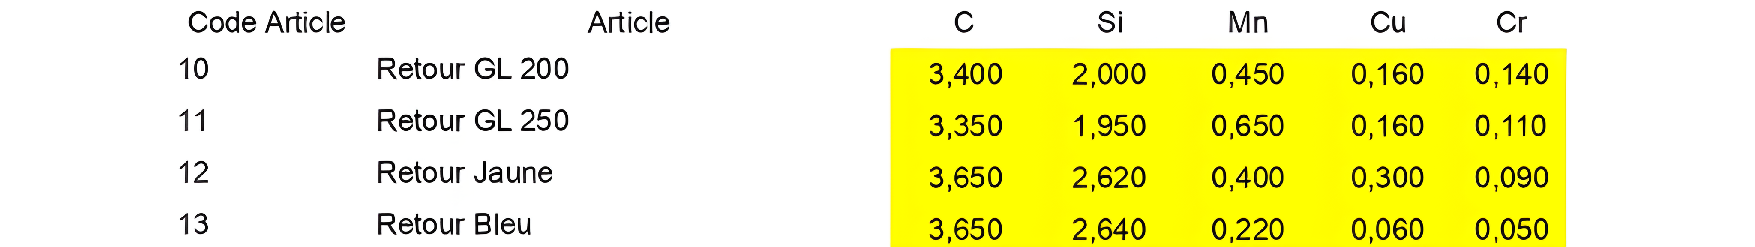
\includegraphics[width=\textwidth]{Images/Recette/Tableau matières premières 1-1.pdf} \\
            \vspace{0.01 cm}
            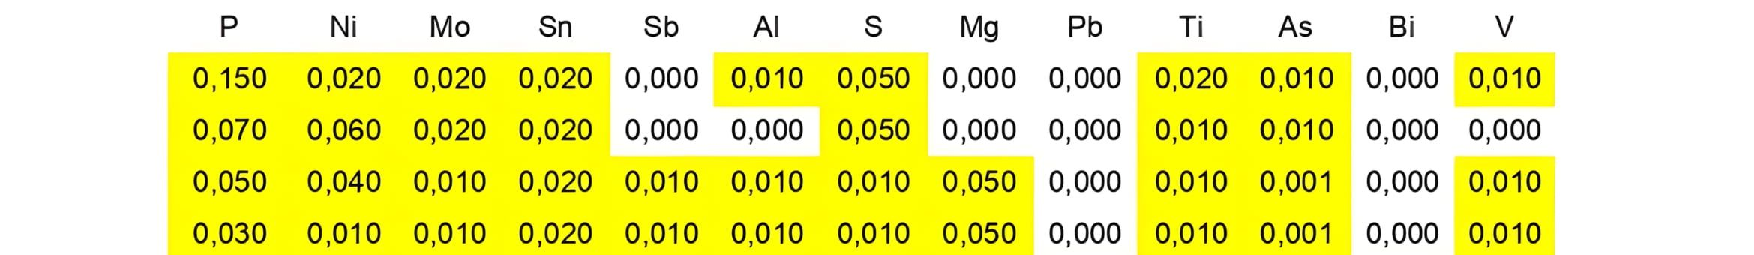
\includegraphics[width=\textwidth]{Images/Recette/Tableau matières premières 1-2.pdf}
        \end{minipage}
    }
    \caption{Illustration du tableau matières premières}
    \label{fig:contraintes1}
\end{figure}



% Les contraintes qualités de la GS 400-15 et de la GS 450-10
\begin{figure}[H]
    \centering
    \adjustbox{width=1.3\textwidth, center}{
        \begin{minipage}{\textwidth}
            \centering
            \includegraphics[width=0.75\paperwidth]{Images/Recette/Contraintes Qualités GS_400_15_1.pdf} \\
            \vspace{0.01 cm}
            \includegraphics[width=0.75\paperwidth]{Images/Recette/Contraintes Qualités GS_400_15_2.pdf}  \\
            \vspace{0.5 cm}
            \includegraphics[width=0.75\paperwidth]{Images/Recette/Contraintes Qualités GS_450_10_1.pdf}  \\
            \vspace{0.01 cm}
            \includegraphics[width=0.75\paperwidth]{Images/Recette/Contraintes Qualités GS_450_10_2.pdf}  
        \end{minipage}
    }
    \caption{Les contraintes qualités de la fonte GS 400-15 et GS 450-10}
    \label{fig:contraintes2}
\end{figure}


% Les contraintes matières premières
\begin{figure}[H]
    \centering
    \begin{adjustbox}{width=1.25\textwidth,center}
        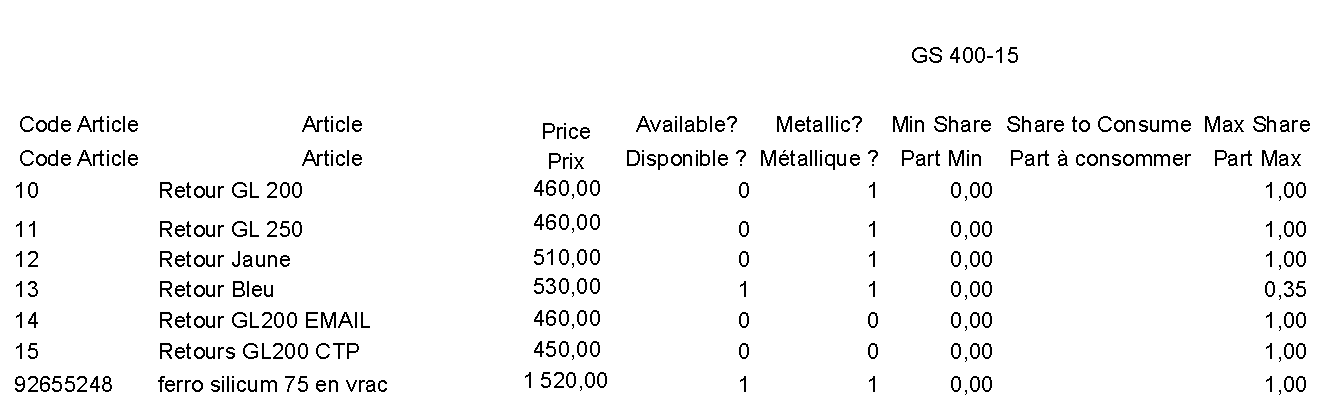
\includegraphics[scale=1]{Images/Recette/Contraintes matières premières 1.pdf}
    \end{adjustbox}
    \caption{Les contraintes matières premières}
    \label{fig:contraintes3}
\end{figure}





%  Les ouputs de l'algos



% \subsection{Mise en oeuvre de la méthode du simplexe}

% Fonction create_optimal_recipe

% \begin{lstlisting}[style=python]
% \begin{lstlisting}[fragile]

\begin{lstlisting}[style=python]
    def create_optimal_recipe(recette,table_mp, mp_constraints, elmt_quality_constraints,dossier_data):
        df_mp, df_elmt_and_quality = mp_constraints[recette], elmt_quality_constraints[recette]
        df_contraints_element, df_contraints_qualite, df_mp_dispo, df_mp_indispo = Separate_data(table_mp, df_mp, df_elmt_and_quality)
        # Suppression des matières premières indisponibles
        table_mp = clean_table_mp(table_mp, df_mp_indispo)
        # Construction de la matrice A et du vecteur C
        A, C = create_matrix_A_and_C(table_mp, df_mp_dispo)
        # Initialisation des listes pour les contraintes
        constraints = {'A_eq': {},'b_eq': {},'A_sup': {},'b_sup': {} }
        # contraintes concernant les éléments chimiques
        constraints = format_constraints_elements(df_contraints_element, A, constraints)
        # contraintes concernant la qualité
        constraints = format_constraints_qualite(df_contraints_qualite, A, constraints)
        # contraintes concernant les matières premières disponibles
        constraints, bounds = format_constraints_MP(df_mp_dispo, constraints)
        # Résoudre le problème d'optimisation linéaire
        method = 'simplex' 
        res, erreurs = solve_linear_program(C, constraints, bounds, method)
        # Gestion du résultat
        gestion_resultats(erreurs, res, df_mp_dispo, table_mp, 
                        constraints, dossier_data, recette)
        return
\end{lstlisting}
    








\section{Le Traitement au Magnésium de la fonte GS}

\subsection{Présentation du problème }



-  On cherche


Voici une reformulation plus claire et lisible de votre texte :

Dans cette partie, nous nous concentrons sur la production de fonte à 
graphite sphéroïdal (GS) réalisée par le processus DISAMATIC, en 
particulier sur l’étape de sphéroïdisation. Cette étape consiste 
principalement à ajouter du magnésium (Mg) à la fonte avant la coulée. 
Le magnésium est introduit sous forme d'alliage en utilisant un fil fourré.

À la fonderie, le coût du fil fourré est de 6,68 € par kilogramme de poudre,
avec une masse de 418 g par mètre de fil. La quantité de magnésium contenue
dans ce fil est de 43 g par mètre.

Avant d'ajouter le fil fourré à la fonte, il est nécessaire de produire 
cette dernière. La fonderie dispose de deux fours de fusion d'une capacité 
de 5 tonnes chacun. Le processus de préparation du lit de fusion, qui 
consiste à charger les matières premières, prend 25 minutes, tandis que 
la fusion des matières premières dure 45 minutes.
On suppose le pourcentage de Mg est nul dans la fonte fournis par le four de 
Fusion. 


Une fois la fonte créée, elle est versée et transportée dans des 
poches. Il existe deux types de poches utilisées : une poche de traitement 
et une poche de coulée, chacune pouvant contenir jusqu'à 1250 kg de fonte.
La fonte sera ensuite recu dans le Four de Coullée.


Concernant le four de coulée, certaines règles spécifiques doivent être 
respectées. Le four, d'une capacité maximale de 5 tonnes, doit toujours 
contenir au moins 2500 kg de fonte. Si cette quantité minimale n'est pas 
respectée, cela pourrait endommager le four. C’est pourquoi la production 
des moules ne commence qu’après l’ajout de la troisième poche de fonte.

Le pourcentage de magnésium (Mg) doit être compris entre 0,035 \% et 
0,045 \%. Cette contrainte sur la teneur en magnésium garantit la qualité 
de la pièce finale tout en minimisant le coût du fil fourré.

En général, dans le programme des pièces à réaliser dans la journée, 
le type, la taille et la quantité des pièces varient. Cela entraîne des 
variations dans le nombre de mottes à réaliser, la masse des grappes et 
le nombre de moules produits par heure.




% -----------




On a une donnée d'entrée : la candence et la poids de motte. On sait ce que 
l'on consomme, c'est ca la fonction de consommation. Cette consommation de 
fonte permet de savoir combien de temps l'on met pour passer de 3500 kg à 
2500 kg de fonte dans le four de Coulée. On veut savoir à quel moment, on 
doit lancer la prochaine poche de traitement. Cette poche doit arriver avant
que la fonte dans le Four de Coulée atteingne son mininum 2500. Si le 
mininum est depasse cela peut endomager le four de Coulée.



On a une fonction de perte du Mg en fonction du temps.
Dans le Four de Coullée, le pourcentage de Mg doit etre compris entre à 
0.035 - 0.045 \% cette contrainte sur le mg permet de garantir la qualité 
de la pièce finale tout en limitant le prix du fil Fourre.


But : Trouver la quantite de Mg à mettre dans chaque poche de traitement
qui permettera au Four de Coullée de retrouver le pourcentage maximale de Mg
fixée à 0.045. La durrée du Traitement MG est d'environ 10 minutes, 
c'est-à-dire la fonte met 10 minutes de la Fusion au Four de coulée.



L'un des objectif de ce problème 
est de trouver la longueur en mettre optimal de fil fourre utiliser. 

% Le Traitement GS


% Les Poches MG 1 et 2 et 3
\begin{figure}[H]
    \centering
    \begin{adjustbox}{height=0.49\textheight,width=1.25\textwidth,center}
        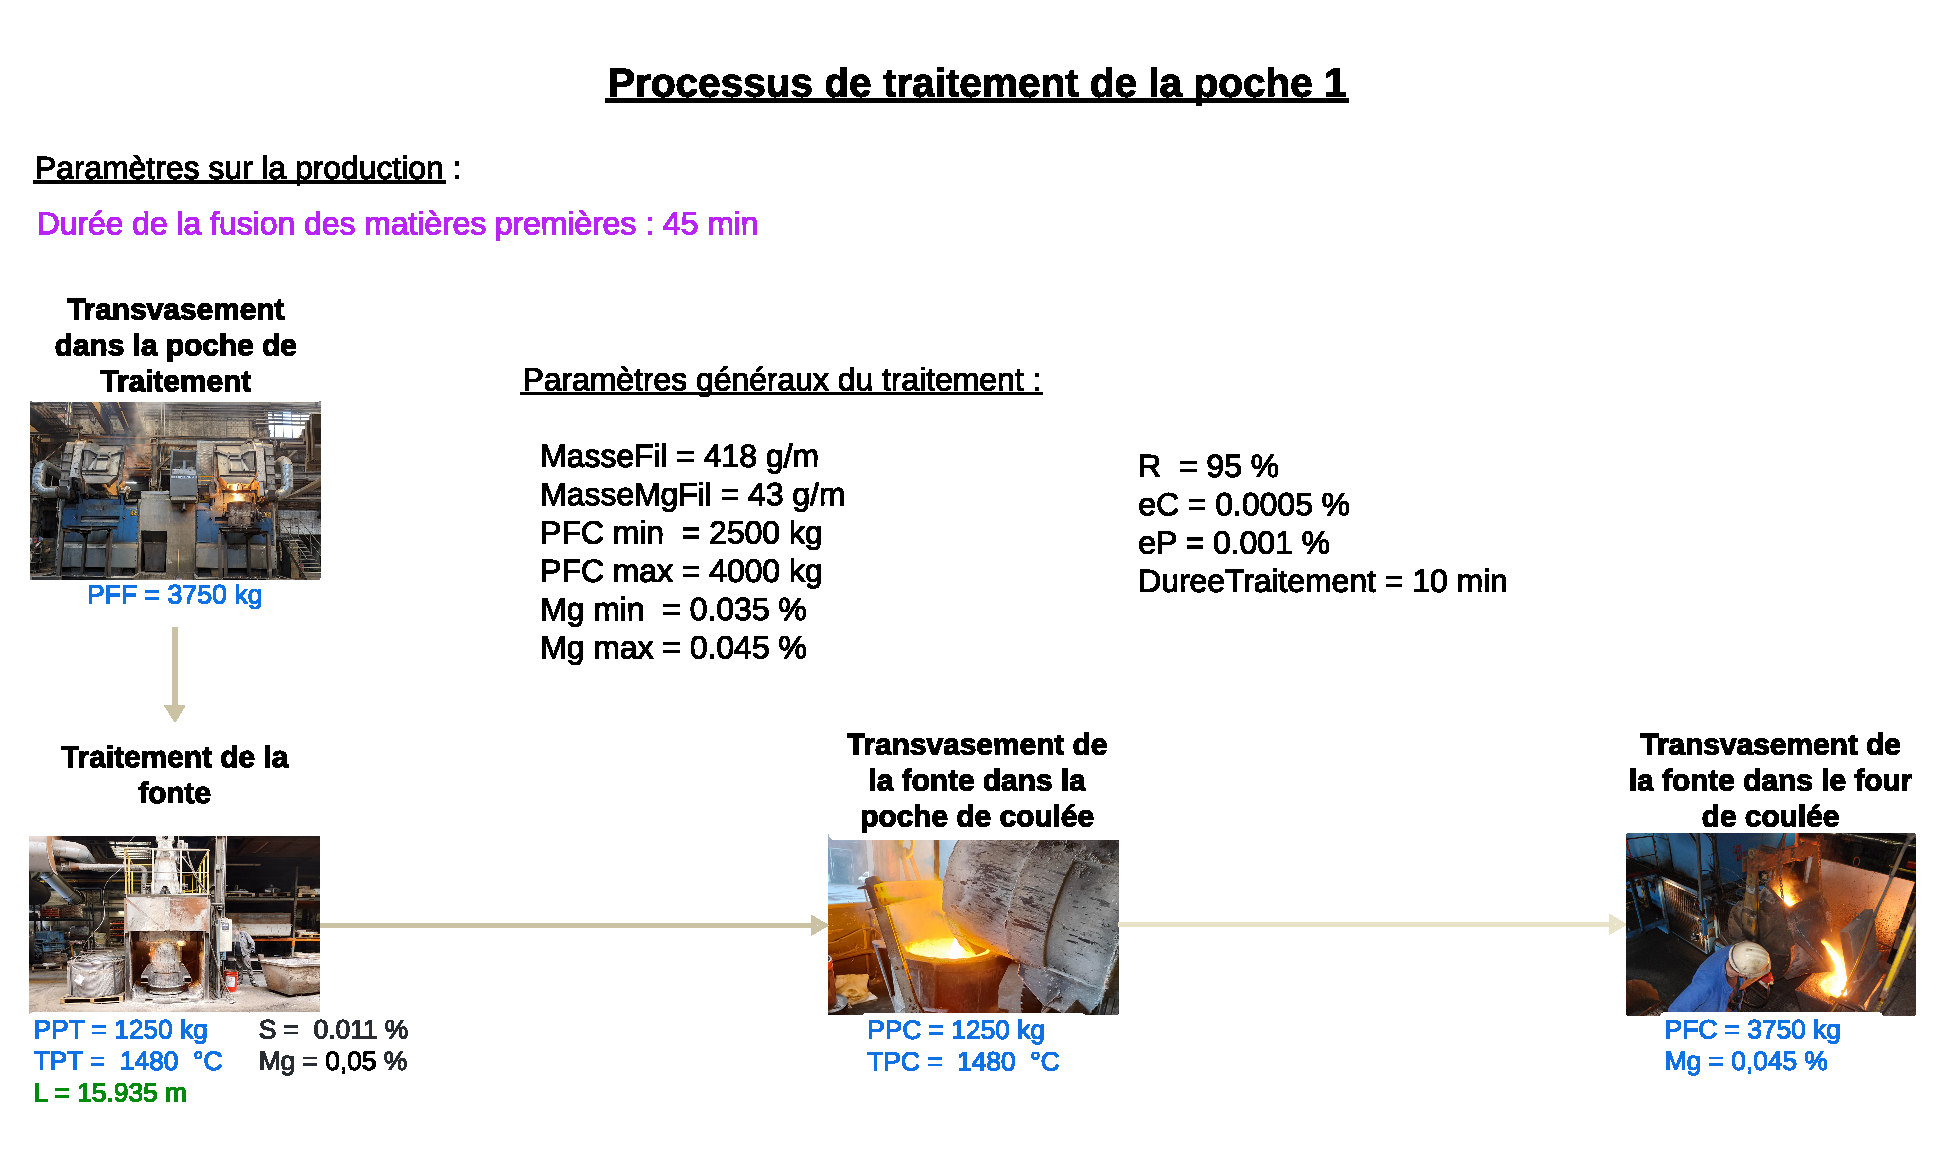
\includegraphics{Images/Mg/Poche 1.pdf} % Première image
    \end{adjustbox}
    
    \vspace{0.01cm} % Espacement entre les images
    
    \begin{adjustbox}{height=0.49\textheight,width=1.25\textwidth,center}
        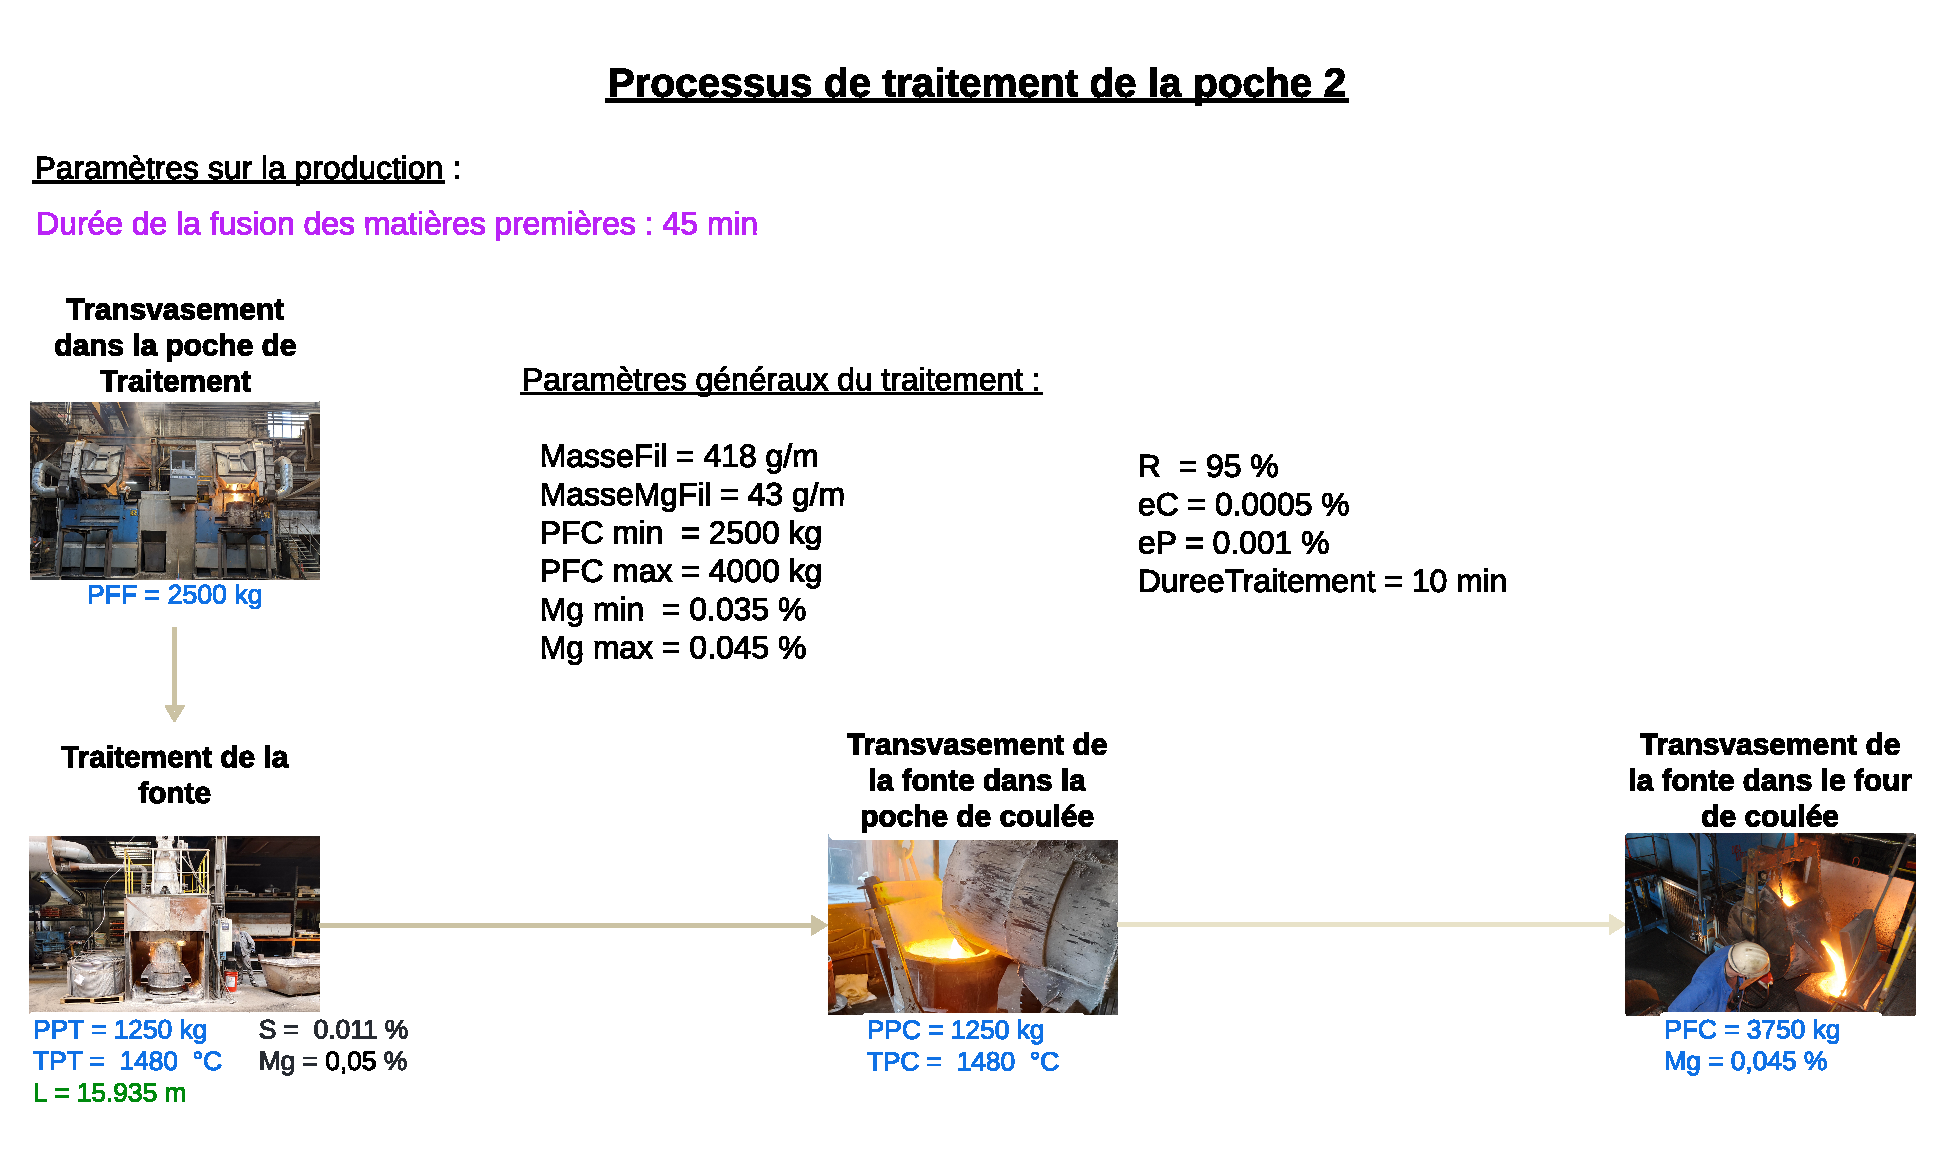
\includegraphics{Images/Mg/Poche 2.pdf} % Deuxième image
    \end{adjustbox}

    \caption{Le Traitement au MG des Poche 1 et Poche 2}
    \label{fig:Poche1Et2}
\end{figure}



\begin{figure}[H]
    \centering
    \begin{adjustbox}{width=1.3\textwidth,center}
        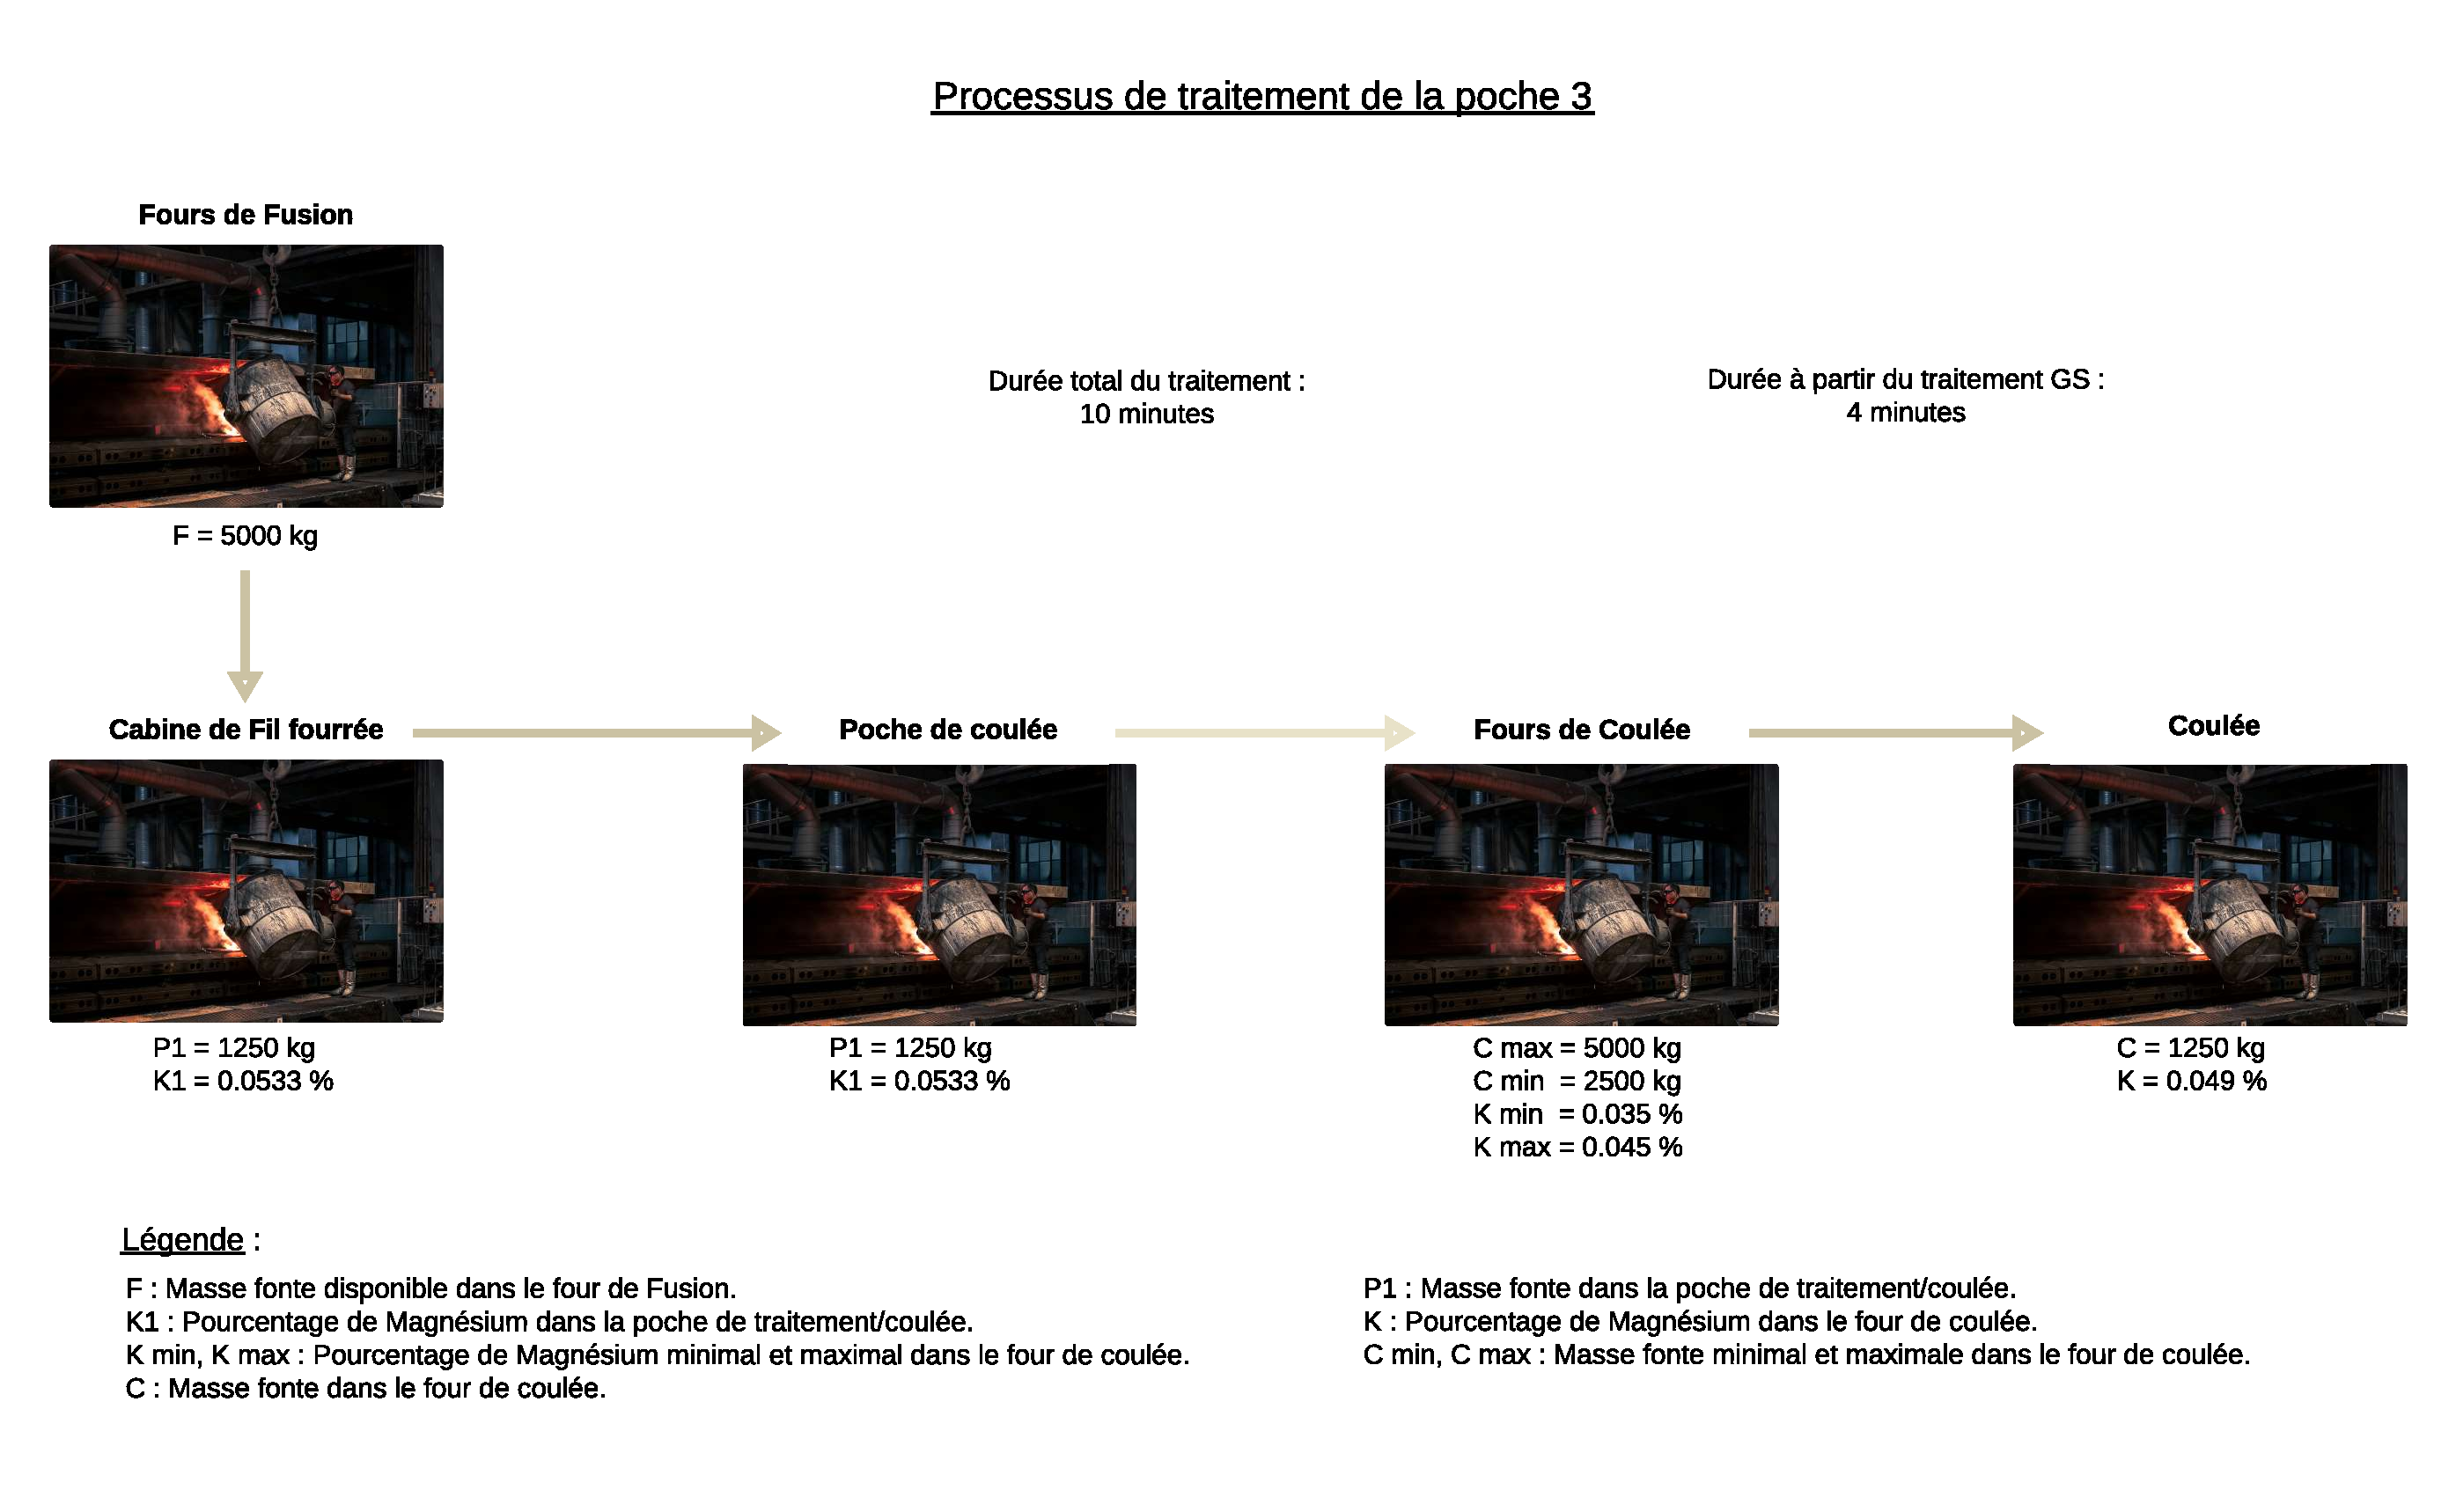
\includegraphics{Images/Mg/Poche 3.pdf}
    \end{adjustbox}
    \caption{Le Traitement au MG de la Poche 3}
    \label{fig:Poche3}
\end{figure}



\subsection{Résolutions du problème}


% Le Traitement GS
Pour calculer la quantité d'alliages au magnésium à introduire dans la poche, on utilise la relation empirique suivante :

$$
\mathbf{Q} = \mathbf{P} \cdot \frac{0.76 (\mathbf{S} - 0.01) + \mathbf{K} + \mathbf{t} \cdot \mathbf{eP}}{\frac{\mathbf{R} \cdot \mathbf{Mg}}{100}} \cdot \left(\frac{\mathbf{T}}{1450}\right)^2
$$

\textbf{Variables et paramètres :}

\begin{itemize}
    \item \textbf{Q} : Quantité d'alliage au magnésium à utiliser (en kg)
    \item \textbf{P} : Poids de fonte à traiter (en kg)
    \item \textbf{S} : Taux de soufre de la fonte de base (en \%)
    \item \textbf{t} : Temps de séjour prévu pour la fonte après traitement (en minutes)
    \item \textbf{eP} : Pourcentage de perte de magnésium par minute dans la poche (\%)
    \item \textbf{T} : Température de la fonte au moment du traitement (en degrés Celsius)
    \item \textbf{R} : Rendement en magnésium de l'opération (en \%)
    \item \textbf{Mg} : Taux de magnésium dans l'alliage (en \%)
    \item \textbf{K} : Quantité de magnésium résiduel nécessaire pour que le graphite soit sous forme sphéroïdal (en \%)
\end{itemize}






Phase Tansitoire 

- Explication de cette phase 


- Obtention des images inputs, outpouts Optimisation de la Presentations
Dans le drive , exporter en pdf avec parametre Paysage, Statement, dessus puis bas






\subsection{Résultats}
    




% \begin{table}[H]
%     \caption{Tableau 1.5: Composition chimique des fontes GS (ADI) [26]}
%     \centering
%         \begin{tabular}{|c|c|}
%         \hline
%         Nuance & Carbone [\%] \\ \hline
%         GS 400-15 & 3.50-4.00  \\ \hline
%         GS 450-10 & 3.50-4.00  \\ \hline
%         \end{tabular}
% \end{table}
    
% sudo apt-get install texlive-full
    
% \begin{table}[H]
% \caption{Tableau 1.5: composition chimique des fontes GS (ADI) [26]}
%     \begin{tabular}{|l|l|l|l|l|l|l|}
%     \hline
%     Nuance & Carbone (\%) & Silicium (\%) & Manganèse (\%) & Phosphore (\%) & Soufre (\%) & Magnésium (\%) & Cuivre (\%) \\ \hline
%     FGS400-15 & 3.50-4.00 & 2.50-2.80 & <0.30 & 4.30-4.95 & <0.06 & <0.20 \\ \hline
%     FGS450-10 & 3.50-4.00 & 2.50-2.88 & <0.45 & 4.30-4.90 & <0.06 & <0.20 \\ \hline
%     \end{tabular}
% \end{table}




\begin{thebibliography}{9}

\bibitem{Gianluigi Rozza}
Gianluigi Rozza.  \emph{An introduction to reduced basis method for parametrized PDEs, ResearchGate}

\bibitem{B. Haasdonk}
B. Haasdonk.  \emph{Reduced Basis Methods for Parametrized PDEs –
A Tutorial Introduction for Stationary and
Instationary Problems, University of Stuttgart  } 


\bibitem{Alexandre Ern}

\bibitem{Bopeng RAO}
Bopeng RAO,  \emph{ Méthodes Numériques
des Equations aux Dérivées Partielles. UFR de Mathématique et d’Informatique
Université de Strasbourg, 2021-2022 }

\bibitem{Gwenol Grandperrin}
Gwenol Grandperrin.  \emph{Introduction à la méthode des bases réduites, ResearchGate Janvier 2008 }


Dantzig, George B. Linear Programming and Extensions. Princeton University Press, 1963.

\end{thebibliography}

\end{document}